\documentclass[11pt]{article}

    \usepackage[breakable]{tcolorbox}
    \usepackage{parskip} % Stop auto-indenting (to mimic markdown behaviour)
\usepackage[utf8]{inputenc}
\usepackage[T1]{fontenc}
\usepackage[ngerman]{babel}
    

    % Basic figure setup, for now with no caption control since it's done
    % automatically by Pandoc (which extracts ![](path) syntax from Markdown).
    \usepackage{graphicx}
    % Keep aspect ratio if custom image width or height is specified
    \setkeys{Gin}{keepaspectratio}
    % Maintain compatibility with old templates. Remove in nbconvert 6.0
    \let\Oldincludegraphics\includegraphics
    % Ensure that by default, figures have no caption (until we provide a
    % proper Figure object with a Caption API and a way to capture that
    % in the conversion process - todo).
    \usepackage{caption}
    \DeclareCaptionFormat{nocaption}{}
    \captionsetup{format=nocaption,aboveskip=0pt,belowskip=0pt}

    \usepackage{float}
    \floatplacement{figure}{H} % forces figures to be placed at the correct location
    \usepackage{xcolor} % Allow colors to be defined
    \usepackage{enumerate} % Needed for markdown enumerations to work
    \usepackage{geometry} % Used to adjust the document margins
    \usepackage{amsmath} % Equations
    \usepackage{amssymb} % Equations
    \usepackage{textcomp} % defines textquotesingle
    % Hack from http://tex.stackexchange.com/a/47451/13684:
    \AtBeginDocument{%
        \def\PYZsq{\textquotesingle}% Upright quotes in Pygmentized code
    }
    \usepackage{upquote} % Upright quotes for verbatim code
    \usepackage{eurosym} % defines \euro

    \usepackage{iftex}
    \ifPDFTeX
        \usepackage[T1]{fontenc}
        \IfFileExists{alphabeta.sty}{
              \usepackage{alphabeta}
          }{
              \usepackage[mathletters]{ucs}
              % \usepackage[utf8x]{inputenc}
          }
    \else
        \usepackage{fontspec}
        \usepackage{unicode-math}
    \fi

    \usepackage{fancyvrb} % verbatim replacement that allows latex
    \usepackage{grffile} % extends the file name processing of package graphics
                         % to support a larger range
    \makeatletter % fix for old versions of grffile with XeLaTeX
    \@ifpackagelater{grffile}{2019/11/01}
    {
      % Do nothing on new versions
    }
    {
      \def\Gread@@xetex#1{%
        \IfFileExists{"\Gin@base".bb}%
        {\Gread@eps{\Gin@base.bb}}%
        {\Gread@@xetex@aux#1}%
      }
    }
    \makeatother
    \usepackage[Export]{adjustbox} % Used to constrain images to a maximum size
    \adjustboxset{max size={0.9\linewidth}{0.9\paperheight}}

    % The hyperref package gives us a pdf with properly built
    % internal navigation ('pdf bookmarks' for the table of contents,
    % internal cross-reference links, web links for URLs, etc.)
    \usepackage{hyperref}
    \usepackage{xurl}
    % The default LaTeX title has an obnoxious amount of whitespace. By default,
    % titling removes some of it. It also provides customization options.
    \usepackage{titling}
    \usepackage{longtable} % longtable support required by pandoc >1.10
    \usepackage{booktabs}  % table support for pandoc > 1.12.2
    \usepackage{array}     % table support for pandoc >= 2.11.3
    \usepackage{calc}      % table minipage width calculation for pandoc >= 2.11.1
    \usepackage[inline]{enumitem} % IRkernel/repr support (it uses the enumerate* environment)
    \usepackage[normalem]{ulem} % ulem is needed to support strikethroughs (\sout)
                                % normalem makes italics be italics, not underlines
    \usepackage{soul}      % strikethrough (\st) support for pandoc >= 3.0.0
    \usepackage{mathrsfs}
    

    
    % Colors for the hyperref package
    \definecolor{urlcolor}{rgb}{0,.145,.698}
    \definecolor{linkcolor}{rgb}{.71,0.21,0.01}
    \definecolor{citecolor}{rgb}{.12,.54,.11}

    % ANSI colors
    \definecolor{ansi-black}{HTML}{3E424D}
    \definecolor{ansi-black-intense}{HTML}{282C36}
    \definecolor{ansi-red}{HTML}{E75C58}
    \definecolor{ansi-red-intense}{HTML}{B22B31}
    \definecolor{ansi-green}{HTML}{00A250}
    \definecolor{ansi-green-intense}{HTML}{007427}
    \definecolor{ansi-yellow}{HTML}{DDB62B}
    \definecolor{ansi-yellow-intense}{HTML}{B27D12}
    \definecolor{ansi-blue}{HTML}{208FFB}
    \definecolor{ansi-blue-intense}{HTML}{0065CA}
    \definecolor{ansi-magenta}{HTML}{D160C4}
    \definecolor{ansi-magenta-intense}{HTML}{A03196}
    \definecolor{ansi-cyan}{HTML}{60C6C8}
    \definecolor{ansi-cyan-intense}{HTML}{258F8F}
    \definecolor{ansi-white}{HTML}{C5C1B4}
    \definecolor{ansi-white-intense}{HTML}{A1A6B2}
    \definecolor{ansi-default-inverse-fg}{HTML}{FFFFFF}
    \definecolor{ansi-default-inverse-bg}{HTML}{000000}

    % common color for the border for error outputs.
    \definecolor{outerrorbackground}{HTML}{FFDFDF}

    % commands and environments needed by pandoc snippets
    % extracted from the output of `pandoc -s`
    \providecommand{\tightlist}{%
      \setlength{\itemsep}{0pt}\setlength{\parskip}{0pt}}
    \DefineVerbatimEnvironment{Highlighting}{Verbatim}{commandchars=\\\{\}}
    % Add ',fontsize=\small' for more characters per line
    \newenvironment{Shaded}{}{}
    \newcommand{\KeywordTok}[1]{\textcolor[rgb]{0.00,0.44,0.13}{\textbf{{#1}}}}
    \newcommand{\DataTypeTok}[1]{\textcolor[rgb]{0.56,0.13,0.00}{{#1}}}
    \newcommand{\DecValTok}[1]{\textcolor[rgb]{0.25,0.63,0.44}{{#1}}}
    \newcommand{\BaseNTok}[1]{\textcolor[rgb]{0.25,0.63,0.44}{{#1}}}
    \newcommand{\FloatTok}[1]{\textcolor[rgb]{0.25,0.63,0.44}{{#1}}}
    \newcommand{\CharTok}[1]{\textcolor[rgb]{0.25,0.44,0.63}{{#1}}}
    \newcommand{\StringTok}[1]{\textcolor[rgb]{0.25,0.44,0.63}{{#1}}}
    \newcommand{\CommentTok}[1]{\textcolor[rgb]{0.38,0.63,0.69}{\textit{{#1}}}}
    \newcommand{\OtherTok}[1]{\textcolor[rgb]{0.00,0.44,0.13}{{#1}}}
    \newcommand{\AlertTok}[1]{\textcolor[rgb]{1.00,0.00,0.00}{\textbf{{#1}}}}
    \newcommand{\FunctionTok}[1]{\textcolor[rgb]{0.02,0.16,0.49}{{#1}}}
    \newcommand{\RegionMarkerTok}[1]{{#1}}
    \newcommand{\ErrorTok}[1]{\textcolor[rgb]{1.00,0.00,0.00}{\textbf{{#1}}}}
    \newcommand{\NormalTok}[1]{{#1}}

    % Additional commands for more recent versions of Pandoc
    \newcommand{\ConstantTok}[1]{\textcolor[rgb]{0.53,0.00,0.00}{{#1}}}
    \newcommand{\SpecialCharTok}[1]{\textcolor[rgb]{0.25,0.44,0.63}{{#1}}}
    \newcommand{\VerbatimStringTok}[1]{\textcolor[rgb]{0.25,0.44,0.63}{{#1}}}
    \newcommand{\SpecialStringTok}[1]{\textcolor[rgb]{0.73,0.40,0.53}{{#1}}}
    \newcommand{\ImportTok}[1]{{#1}}
    \newcommand{\DocumentationTok}[1]{\textcolor[rgb]{0.73,0.13,0.13}{\textit{{#1}}}}
    \newcommand{\AnnotationTok}[1]{\textcolor[rgb]{0.38,0.63,0.69}{\textbf{\textit{{#1}}}}}
    \newcommand{\CommentVarTok}[1]{\textcolor[rgb]{0.38,0.63,0.69}{\textbf{\textit{{#1}}}}}
    \newcommand{\VariableTok}[1]{\textcolor[rgb]{0.10,0.09,0.49}{{#1}}}
    \newcommand{\ControlFlowTok}[1]{\textcolor[rgb]{0.00,0.44,0.13}{\textbf{{#1}}}}
    \newcommand{\OperatorTok}[1]{\textcolor[rgb]{0.40,0.40,0.40}{{#1}}}
    \newcommand{\BuiltInTok}[1]{{#1}}
    \newcommand{\ExtensionTok}[1]{{#1}}
    \newcommand{\PreprocessorTok}[1]{\textcolor[rgb]{0.74,0.48,0.00}{{#1}}}
    \newcommand{\AttributeTok}[1]{\textcolor[rgb]{0.49,0.56,0.16}{{#1}}}
    \newcommand{\InformationTok}[1]{\textcolor[rgb]{0.38,0.63,0.69}{\textbf{\textit{{#1}}}}}
    \newcommand{\WarningTok}[1]{\textcolor[rgb]{0.38,0.63,0.69}{\textbf{\textit{{#1}}}}}
    \makeatletter
    \newsavebox\pandoc@box
    \newcommand*\pandocbounded[1]{%
      \sbox\pandoc@box{#1}%
      % scaling factors for width and height
      \Gscale@div\@tempa\textheight{\dimexpr\ht\pandoc@box+\dp\pandoc@box\relax}%
      \Gscale@div\@tempb\linewidth{\wd\pandoc@box}%
      % select the smaller of both
      \ifdim\@tempb\p@<\@tempa\p@
        \let\@tempa\@tempb
      \fi
      % scaling accordingly (\@tempa < 1)
      \ifdim\@tempa\p@<\p@
        \scalebox{\@tempa}{\usebox\pandoc@box}%
      % scaling not needed, use as it is
      \else
        \usebox{\pandoc@box}%
      \fi
    }
    \makeatother

    % Define a nice break command that doesn't care if a line doesn't already
    % exist.
    \def\br{\hspace*{\fill} \\* }
    % Math Jax compatibility definitions
    \def\gt{>}
    \def\lt{<}
    \let\Oldtex\TeX
    \let\Oldlatex\LaTeX
    \renewcommand{\TeX}{\textrm{\Oldtex}}
    \renewcommand{\LaTeX}{\textrm{\Oldlatex}}
    % Document parameters
    % Document title
    \title{Scientific Programming Lab - Erde und Mond}
    \author{Lara Artmann\and Viktoria Backhaus\and Bekir Taha Gede\and Sheila Kaiser\and Darian Mark\and Luke Munderich}
    
    
    
    
    
    
    
% Pygments definitions
\makeatletter
\def\PY@reset{\let\PY@it=\relax \let\PY@bf=\relax%
    \let\PY@ul=\relax \let\PY@tc=\relax%
    \let\PY@bc=\relax \let\PY@ff=\relax}
\def\PY@tok#1{\csname PY@tok@#1\endcsname}
\def\PY@toks#1+{\ifx\relax#1\empty\else%
    \PY@tok{#1}\expandafter\PY@toks\fi}
\def\PY@do#1{\PY@bc{\PY@tc{\PY@ul{%
    \PY@it{\PY@bf{\PY@ff{#1}}}}}}}
\def\PY#1#2{\PY@reset\PY@toks#1+\relax+\PY@do{#2}}

\@namedef{PY@tok@w}{\def\PY@tc##1{\textcolor[rgb]{0.73,0.73,0.73}{##1}}}
\@namedef{PY@tok@c}{\let\PY@it=\textit\def\PY@tc##1{\textcolor[rgb]{0.24,0.48,0.48}{##1}}}
\@namedef{PY@tok@cp}{\def\PY@tc##1{\textcolor[rgb]{0.61,0.40,0.00}{##1}}}
\@namedef{PY@tok@k}{\let\PY@bf=\textbf\def\PY@tc##1{\textcolor[rgb]{0.00,0.50,0.00}{##1}}}
\@namedef{PY@tok@kp}{\def\PY@tc##1{\textcolor[rgb]{0.00,0.50,0.00}{##1}}}
\@namedef{PY@tok@kt}{\def\PY@tc##1{\textcolor[rgb]{0.69,0.00,0.25}{##1}}}
\@namedef{PY@tok@o}{\def\PY@tc##1{\textcolor[rgb]{0.40,0.40,0.40}{##1}}}
\@namedef{PY@tok@ow}{\let\PY@bf=\textbf\def\PY@tc##1{\textcolor[rgb]{0.67,0.13,1.00}{##1}}}
\@namedef{PY@tok@nb}{\def\PY@tc##1{\textcolor[rgb]{0.00,0.50,0.00}{##1}}}
\@namedef{PY@tok@nf}{\def\PY@tc##1{\textcolor[rgb]{0.00,0.00,1.00}{##1}}}
\@namedef{PY@tok@nc}{\let\PY@bf=\textbf\def\PY@tc##1{\textcolor[rgb]{0.00,0.00,1.00}{##1}}}
\@namedef{PY@tok@nn}{\let\PY@bf=\textbf\def\PY@tc##1{\textcolor[rgb]{0.00,0.00,1.00}{##1}}}
\@namedef{PY@tok@ne}{\let\PY@bf=\textbf\def\PY@tc##1{\textcolor[rgb]{0.80,0.25,0.22}{##1}}}
\@namedef{PY@tok@nv}{\def\PY@tc##1{\textcolor[rgb]{0.10,0.09,0.49}{##1}}}
\@namedef{PY@tok@no}{\def\PY@tc##1{\textcolor[rgb]{0.53,0.00,0.00}{##1}}}
\@namedef{PY@tok@nl}{\def\PY@tc##1{\textcolor[rgb]{0.46,0.46,0.00}{##1}}}
\@namedef{PY@tok@ni}{\let\PY@bf=\textbf\def\PY@tc##1{\textcolor[rgb]{0.44,0.44,0.44}{##1}}}
\@namedef{PY@tok@na}{\def\PY@tc##1{\textcolor[rgb]{0.41,0.47,0.13}{##1}}}
\@namedef{PY@tok@nt}{\let\PY@bf=\textbf\def\PY@tc##1{\textcolor[rgb]{0.00,0.50,0.00}{##1}}}
\@namedef{PY@tok@nd}{\def\PY@tc##1{\textcolor[rgb]{0.67,0.13,1.00}{##1}}}
\@namedef{PY@tok@s}{\def\PY@tc##1{\textcolor[rgb]{0.73,0.13,0.13}{##1}}}
\@namedef{PY@tok@sd}{\let\PY@it=\textit\def\PY@tc##1{\textcolor[rgb]{0.73,0.13,0.13}{##1}}}
\@namedef{PY@tok@si}{\let\PY@bf=\textbf\def\PY@tc##1{\textcolor[rgb]{0.64,0.35,0.47}{##1}}}
\@namedef{PY@tok@se}{\let\PY@bf=\textbf\def\PY@tc##1{\textcolor[rgb]{0.67,0.36,0.12}{##1}}}
\@namedef{PY@tok@sr}{\def\PY@tc##1{\textcolor[rgb]{0.64,0.35,0.47}{##1}}}
\@namedef{PY@tok@ss}{\def\PY@tc##1{\textcolor[rgb]{0.10,0.09,0.49}{##1}}}
\@namedef{PY@tok@sx}{\def\PY@tc##1{\textcolor[rgb]{0.00,0.50,0.00}{##1}}}
\@namedef{PY@tok@m}{\def\PY@tc##1{\textcolor[rgb]{0.40,0.40,0.40}{##1}}}
\@namedef{PY@tok@gh}{\let\PY@bf=\textbf\def\PY@tc##1{\textcolor[rgb]{0.00,0.00,0.50}{##1}}}
\@namedef{PY@tok@gu}{\let\PY@bf=\textbf\def\PY@tc##1{\textcolor[rgb]{0.50,0.00,0.50}{##1}}}
\@namedef{PY@tok@gd}{\def\PY@tc##1{\textcolor[rgb]{0.63,0.00,0.00}{##1}}}
\@namedef{PY@tok@gi}{\def\PY@tc##1{\textcolor[rgb]{0.00,0.52,0.00}{##1}}}
\@namedef{PY@tok@gr}{\def\PY@tc##1{\textcolor[rgb]{0.89,0.00,0.00}{##1}}}
\@namedef{PY@tok@ge}{\let\PY@it=\textit}
\@namedef{PY@tok@gs}{\let\PY@bf=\textbf}
\@namedef{PY@tok@ges}{\let\PY@bf=\textbf\let\PY@it=\textit}
\@namedef{PY@tok@gp}{\let\PY@bf=\textbf\def\PY@tc##1{\textcolor[rgb]{0.00,0.00,0.50}{##1}}}
\@namedef{PY@tok@go}{\def\PY@tc##1{\textcolor[rgb]{0.44,0.44,0.44}{##1}}}
\@namedef{PY@tok@gt}{\def\PY@tc##1{\textcolor[rgb]{0.00,0.27,0.87}{##1}}}
\@namedef{PY@tok@err}{\def\PY@bc##1{{\setlength{\fboxsep}{\string -\fboxrule}\fcolorbox[rgb]{1.00,0.00,0.00}{1,1,1}{\strut ##1}}}}
\@namedef{PY@tok@kc}{\let\PY@bf=\textbf\def\PY@tc##1{\textcolor[rgb]{0.00,0.50,0.00}{##1}}}
\@namedef{PY@tok@kd}{\let\PY@bf=\textbf\def\PY@tc##1{\textcolor[rgb]{0.00,0.50,0.00}{##1}}}
\@namedef{PY@tok@kn}{\let\PY@bf=\textbf\def\PY@tc##1{\textcolor[rgb]{0.00,0.50,0.00}{##1}}}
\@namedef{PY@tok@kr}{\let\PY@bf=\textbf\def\PY@tc##1{\textcolor[rgb]{0.00,0.50,0.00}{##1}}}
\@namedef{PY@tok@bp}{\def\PY@tc##1{\textcolor[rgb]{0.00,0.50,0.00}{##1}}}
\@namedef{PY@tok@fm}{\def\PY@tc##1{\textcolor[rgb]{0.00,0.00,1.00}{##1}}}
\@namedef{PY@tok@vc}{\def\PY@tc##1{\textcolor[rgb]{0.10,0.09,0.49}{##1}}}
\@namedef{PY@tok@vg}{\def\PY@tc##1{\textcolor[rgb]{0.10,0.09,0.49}{##1}}}
\@namedef{PY@tok@vi}{\def\PY@tc##1{\textcolor[rgb]{0.10,0.09,0.49}{##1}}}
\@namedef{PY@tok@vm}{\def\PY@tc##1{\textcolor[rgb]{0.10,0.09,0.49}{##1}}}
\@namedef{PY@tok@sa}{\def\PY@tc##1{\textcolor[rgb]{0.73,0.13,0.13}{##1}}}
\@namedef{PY@tok@sb}{\def\PY@tc##1{\textcolor[rgb]{0.73,0.13,0.13}{##1}}}
\@namedef{PY@tok@sc}{\def\PY@tc##1{\textcolor[rgb]{0.73,0.13,0.13}{##1}}}
\@namedef{PY@tok@dl}{\def\PY@tc##1{\textcolor[rgb]{0.73,0.13,0.13}{##1}}}
\@namedef{PY@tok@s2}{\def\PY@tc##1{\textcolor[rgb]{0.73,0.13,0.13}{##1}}}
\@namedef{PY@tok@sh}{\def\PY@tc##1{\textcolor[rgb]{0.73,0.13,0.13}{##1}}}
\@namedef{PY@tok@s1}{\def\PY@tc##1{\textcolor[rgb]{0.73,0.13,0.13}{##1}}}
\@namedef{PY@tok@mb}{\def\PY@tc##1{\textcolor[rgb]{0.40,0.40,0.40}{##1}}}
\@namedef{PY@tok@mf}{\def\PY@tc##1{\textcolor[rgb]{0.40,0.40,0.40}{##1}}}
\@namedef{PY@tok@mh}{\def\PY@tc##1{\textcolor[rgb]{0.40,0.40,0.40}{##1}}}
\@namedef{PY@tok@mi}{\def\PY@tc##1{\textcolor[rgb]{0.40,0.40,0.40}{##1}}}
\@namedef{PY@tok@il}{\def\PY@tc##1{\textcolor[rgb]{0.40,0.40,0.40}{##1}}}
\@namedef{PY@tok@mo}{\def\PY@tc##1{\textcolor[rgb]{0.40,0.40,0.40}{##1}}}
\@namedef{PY@tok@ch}{\let\PY@it=\textit\def\PY@tc##1{\textcolor[rgb]{0.24,0.48,0.48}{##1}}}
\@namedef{PY@tok@cm}{\let\PY@it=\textit\def\PY@tc##1{\textcolor[rgb]{0.24,0.48,0.48}{##1}}}
\@namedef{PY@tok@cpf}{\let\PY@it=\textit\def\PY@tc##1{\textcolor[rgb]{0.24,0.48,0.48}{##1}}}
\@namedef{PY@tok@c1}{\let\PY@it=\textit\def\PY@tc##1{\textcolor[rgb]{0.24,0.48,0.48}{##1}}}
\@namedef{PY@tok@cs}{\let\PY@it=\textit\def\PY@tc##1{\textcolor[rgb]{0.24,0.48,0.48}{##1}}}

\def\PYZbs{\char`\\}
\def\PYZus{\char`\_}
\def\PYZob{\char`\{}
\def\PYZcb{\char`\}}
\def\PYZca{\char`\^}
\def\PYZam{\char`\&}
\def\PYZlt{\char`\<}
\def\PYZgt{\char`\>}
\def\PYZsh{\char`\#}
\def\PYZpc{\char`\%}
\def\PYZdl{\char`\$}
\def\PYZhy{\char`\-}
\def\PYZsq{\char`\'}
\def\PYZdq{\char`\"}
\def\PYZti{\char`\~}
% for compatibility with earlier versions
\def\PYZat{@}
\def\PYZlb{[}
\def\PYZrb{]}
\makeatother


    % For linebreaks inside Verbatim environment from package fancyvrb.
    \makeatletter
        \newbox\Wrappedcontinuationbox
        \newbox\Wrappedvisiblespacebox
        \newcommand*\Wrappedvisiblespace {\textcolor{red}{\textvisiblespace}}
        \newcommand*\Wrappedcontinuationsymbol {\textcolor{red}{\llap{\tiny$\m@th\hookrightarrow$}}}
        \newcommand*\Wrappedcontinuationindent {3ex }
        \newcommand*\Wrappedafterbreak {\kern\Wrappedcontinuationindent\copy\Wrappedcontinuationbox}
        % Take advantage of the already applied Pygments mark-up to insert
        % potential linebreaks for TeX processing.
        %        {, <, #, %, $, ' and ": go to next line.
        %        _, }, ^, &, >, - and ~: stay at end of broken line.
        % Use of \textquotesingle for straight quote.
        \newcommand*\Wrappedbreaksatspecials {%
            \def\PYGZus{\discretionary{\char`\_}{\Wrappedafterbreak}{\char`\_}}%
            \def\PYGZob{\discretionary{}{\Wrappedafterbreak\char`\{}{\char`\{}}%
            \def\PYGZcb{\discretionary{\char`\}}{\Wrappedafterbreak}{\char`\}}}%
            \def\PYGZca{\discretionary{\char`\^}{\Wrappedafterbreak}{\char`\^}}%
            \def\PYGZam{\discretionary{\char`\&}{\Wrappedafterbreak}{\char`\&}}%
            \def\PYGZlt{\discretionary{}{\Wrappedafterbreak\char`\<}{\char`\<}}%
            \def\PYGZgt{\discretionary{\char`\>}{\Wrappedafterbreak}{\char`\>}}%
            \def\PYGZsh{\discretionary{}{\Wrappedafterbreak\char`\#}{\char`\#}}%
            \def\PYGZpc{\discretionary{}{\Wrappedafterbreak\char`\%}{\char`\%}}%
            \def\PYGZdl{\discretionary{}{\Wrappedafterbreak\char`\$}{\char`\$}}%
            \def\PYGZhy{\discretionary{\char`\-}{\Wrappedafterbreak}{\char`\-}}%
            \def\PYGZsq{\discretionary{}{\Wrappedafterbreak\textquotesingle}{\textquotesingle}}%
            \def\PYGZdq{\discretionary{}{\Wrappedafterbreak\char`\"}{\char`\"}}%
            \def\PYGZti{\discretionary{\char`\~}{\Wrappedafterbreak}{\char`\~}}%
        }
        % Some characters . , ; ? ! / are not pygmentized.
        % This macro makes them "active" and they will insert potential linebreaks
        \newcommand*\Wrappedbreaksatpunct {%
            \lccode`\~`\.\lowercase{\def~}{\discretionary{\hbox{\char`\.}}{\Wrappedafterbreak}{\hbox{\char`\.}}}%
            \lccode`\~`\,\lowercase{\def~}{\discretionary{\hbox{\char`\,}}{\Wrappedafterbreak}{\hbox{\char`\,}}}%
            \lccode`\~`\;\lowercase{\def~}{\discretionary{\hbox{\char`\;}}{\Wrappedafterbreak}{\hbox{\char`\;}}}%
            \lccode`\~`\:\lowercase{\def~}{\discretionary{\hbox{\char`\:}}{\Wrappedafterbreak}{\hbox{\char`\:}}}%
            \lccode`\~`\?\lowercase{\def~}{\discretionary{\hbox{\char`\?}}{\Wrappedafterbreak}{\hbox{\char`\?}}}%
            \lccode`\~`\!\lowercase{\def~}{\discretionary{\hbox{\char`\!}}{\Wrappedafterbreak}{\hbox{\char`\!}}}%
            \lccode`\~`\/\lowercase{\def~}{\discretionary{\hbox{\char`\/}}{\Wrappedafterbreak}{\hbox{\char`\/}}}%
            \catcode`\.\active
            \catcode`\,\active
            \catcode`\;\active
            \catcode`\:\active
            \catcode`\?\active
            \catcode`\!\active
            \catcode`\/\active
            \lccode`\~`\~
        }
    \makeatother

    \let\OriginalVerbatim=\Verbatim
    \makeatletter
    \renewcommand{\Verbatim}[1][1]{%
        %\parskip\z@skip
        \sbox\Wrappedcontinuationbox {\Wrappedcontinuationsymbol}%
        \sbox\Wrappedvisiblespacebox {\FV@SetupFont\Wrappedvisiblespace}%
        \def\FancyVerbFormatLine ##1{\hsize\linewidth
            \vtop{\raggedright\hyphenpenalty\z@\exhyphenpenalty\z@
                \doublehyphendemerits\z@\finalhyphendemerits\z@
                \strut ##1\strut}%
        }%
        % If the linebreak is at a space, the latter will be displayed as visible
        % space at end of first line, and a continuation symbol starts next line.
        % Stretch/shrink are however usually zero for typewriter font.
        \def\FV@Space {%
            \nobreak\hskip\z@ plus\fontdimen3\font minus\fontdimen4\font
            \discretionary{\copy\Wrappedvisiblespacebox}{\Wrappedafterbreak}
            {\kern\fontdimen2\font}%
        }%

        % Allow breaks at special characters using \PYG... macros.
        \Wrappedbreaksatspecials
        % Breaks at punctuation characters . , ; ? ! and / need catcode=\active
        \OriginalVerbatim[#1,codes*=\Wrappedbreaksatpunct]%
    }
    \makeatother

    % Exact colors from NB
    \definecolor{incolor}{HTML}{303F9F}
    \definecolor{outcolor}{HTML}{D84315}
    \definecolor{cellborder}{HTML}{CFCFCF}
    \definecolor{cellbackground}{HTML}{F7F7F7}

    % prompt
    \makeatletter
    \newcommand{\boxspacing}{\kern\kvtcb@left@rule\kern\kvtcb@boxsep}
    \makeatother
    \newcommand{\prompt}[4]{
        {\ttfamily\llap{{\color{#2}[#3]:\hspace{3pt}#4}}\vspace{-\baselineskip}}
    }
    

    
    % Prevent overflowing lines due to hard-to-break entities
    \sloppy
    % Setup hyperref package
    \hypersetup{
      breaklinks=true,  % so long urls are correctly broken across lines
      colorlinks=true,
      urlcolor=urlcolor,
      linkcolor=linkcolor,
      citecolor=citecolor,
      }
    % Slightly bigger margins than the latex defaults
    
    \geometry{verbose,tmargin=1in,bmargin=1in,lmargin=1in,rmargin=1in}
    
    

\begin{document}
    
    \maketitle
    
    

    


    \begin{tcolorbox}[breakable, size=fbox, boxrule=1pt, pad at break*=1mm,colback=cellbackground, colframe=cellborder]
\prompt{In}{incolor}{1}{\boxspacing}
\begin{Verbatim}[commandchars=\\\{\}]
\PY{c+c1}{\PYZsh{}Bitte ausführen, damit alles Notwendige importiert wird}
\PY{c+c1}{\PYZsh{}Note: Bei Änderungen der zugrundeliegenden Python\PYZhy{}Files muss Jupyter neugestartet werden}
\PY{k+kn}{import}\PY{+w}{ }\PY{n+nn}{scipro}
\end{Verbatim}
\end{tcolorbox}

    \begin{tcolorbox}[breakable, size=fbox, boxrule=1pt, pad at break*=1mm,colback=cellbackground, colframe=cellborder]
\prompt{In}{incolor}{2}{\boxspacing}
\begin{Verbatim}[commandchars=\\\{\}]
\PY{o}{\PYZpc{}\PYZpc{}html}
\PY{c+cm}{\PYZlt{}!\PYZhy{}\PYZhy{}Bitte diese Cell mit Run ausführen, damit die Styles geladen werden\PYZhy{}\PYZhy{}\PYZgt{}}
\PY{c+cm}{\PYZlt{}!\PYZhy{}\PYZhy{}Bei Änderungen des CSS muss das Notebook im Browser neu geladen werden\PYZhy{}\PYZhy{}\PYZgt{}}
\PY{p}{\PYZlt{}}\PY{n+nt}{link} \PY{n+na}{rel}\PY{o}{=}\PY{l+s}{\PYZdq{}stylesheet\PYZdq{}} \PY{n+na}{href}\PY{o}{=}\PY{l+s}{\PYZdq{}./styles/sciprolab.css\PYZdq{}}\PY{p}{\PYZgt{}}
\end{Verbatim}
\end{tcolorbox}

    
    \begin{Verbatim}[commandchars=\\\{\}]
<IPython.core.display.HTML object>
    \end{Verbatim}

    
    In diesem Jupyter-Notebook soll die Implementierung des Erde-Mond
Systems in Python über Newtons Gravitationsgesetz umgesetzt werden. Es
werden die dahinter liegenden physikalischen Prinzipien erläutert und
die Vorgänge werden visualisiert. Zusätzlich soll ein weiterer Planet
(Theia) das System stören. Theia soll dabei mit verschiedenen
Geschwindigkeiten und aus verschiedenen Richtungen in das System
gelangen.

    \section{Überblick}\label{uxfcberblick}

\begin{figure}
\centering
\pandocbounded{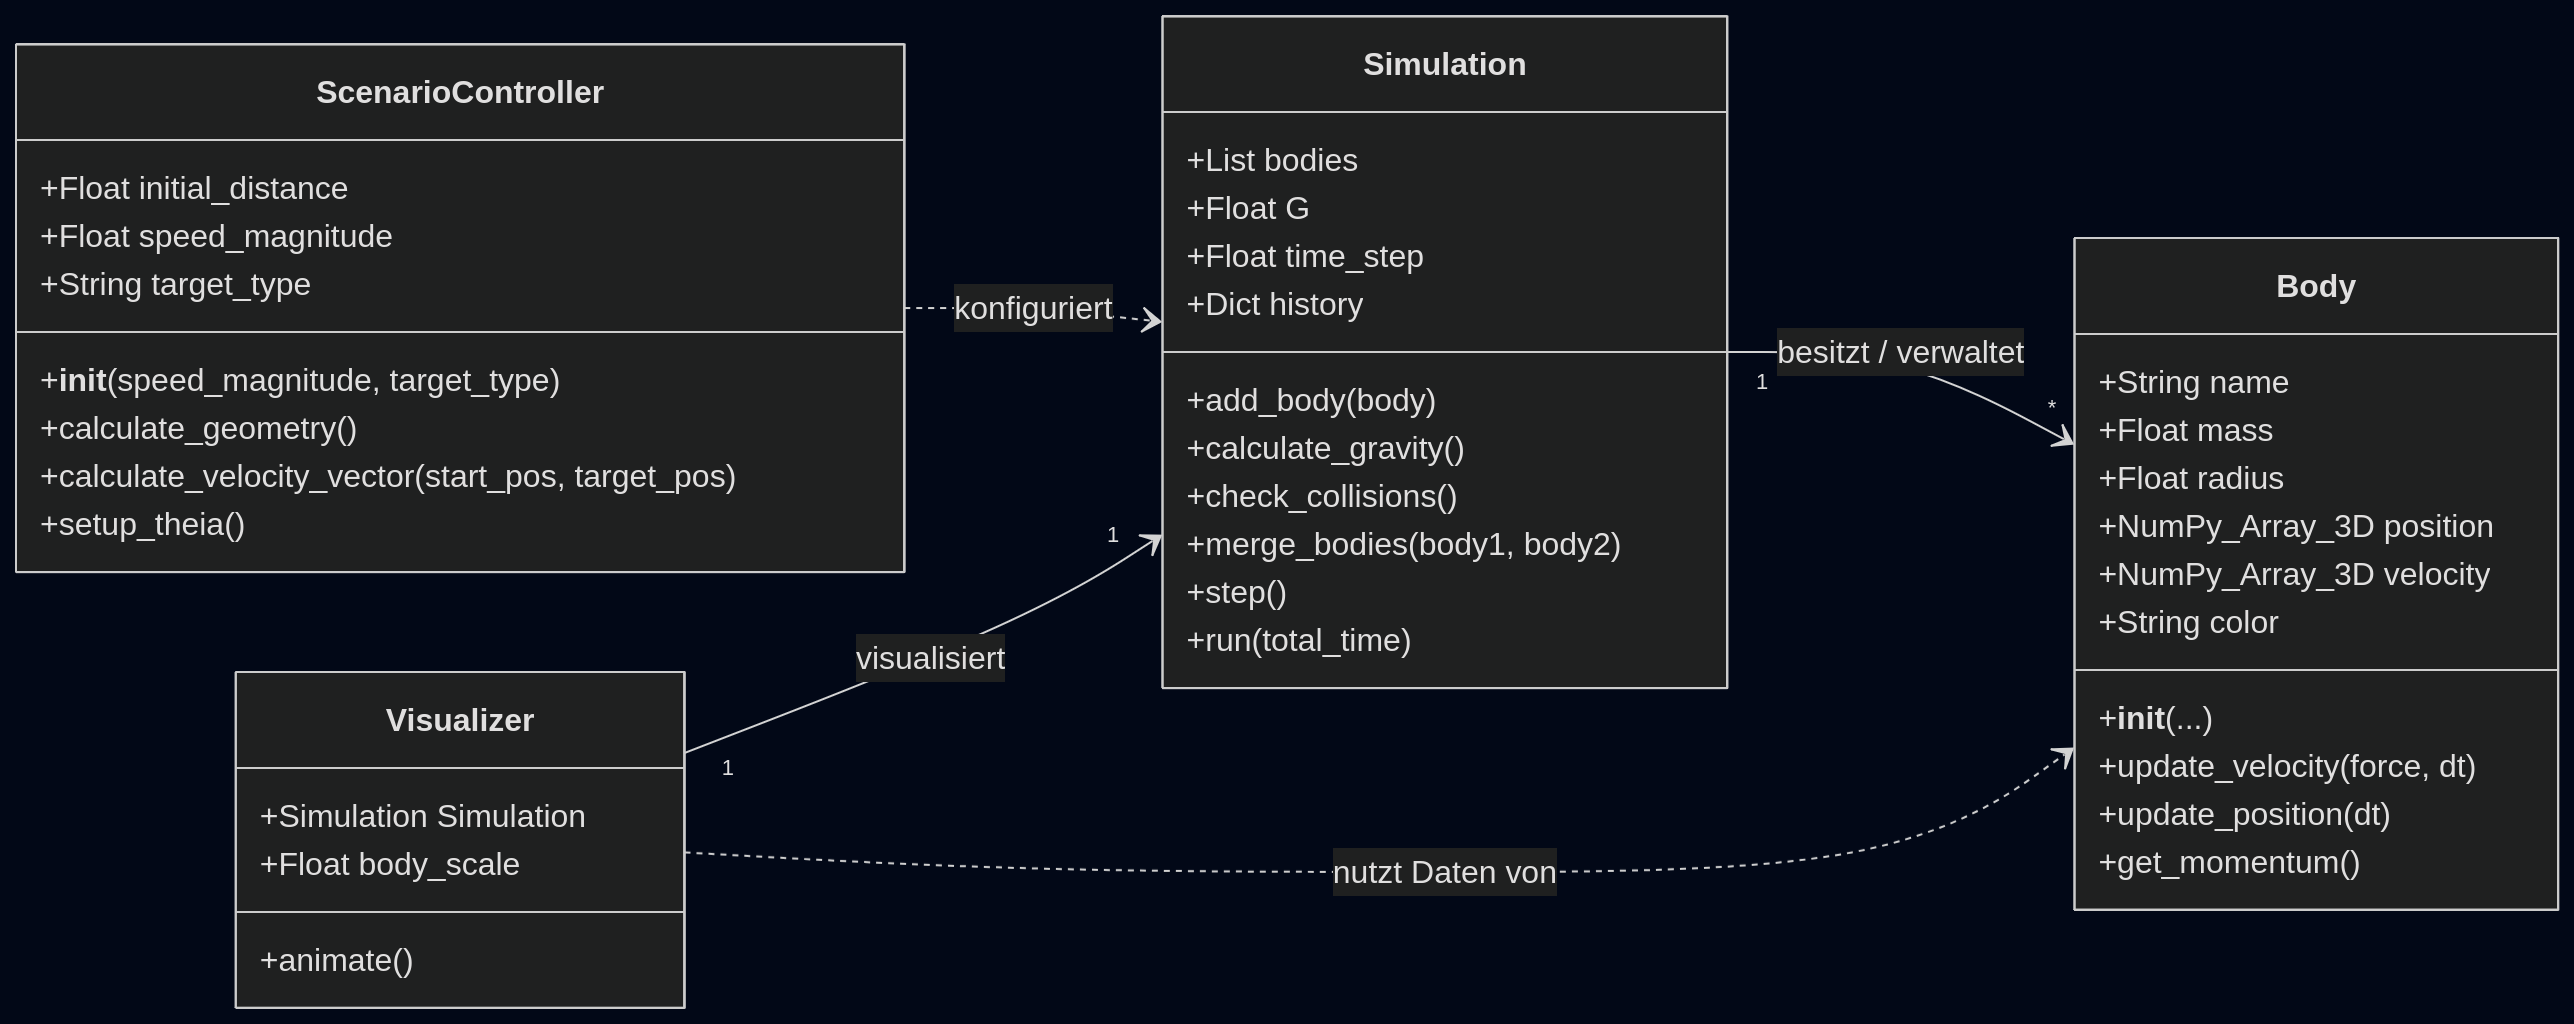
\includegraphics[keepaspectratio]{img/class_diagram.png}}
\caption{Bild}
\end{figure}

    \section{Body Klasse}\label{body-klasse}

Die Klasse representiert einen Himmelskörper in Form einer runden Masse.
Sie bildet den Grundbaustein des Projektes.

\subsection{Mathematische Formeln hinter den
Funktionen:}\label{mathematische-formeln-hinter-den-funktionen}

\paragraph{1. Geometrische
Distanzbestimmung}\label{geometrische-distanzbestimmung}

Der Abstand zwischen zwei Himmelskörpern im dreidimensionalen Raum wird
mithilfe des euklidischen Abstands berechnet.

\begin{verbatim}
  Euklidischer Abstand
\end{verbatim}

\[
d = \|\vec{r}_2 - \vec{r}_1\| = \sqrt{(x_2 - x_1)^2 + (y_2 - y_1)^2 + (z_2 - z_1)^2}
\]

\paragraph{2. Positionsänderung}\label{positionsuxe4nderung}

Es wird die neue Position \(\vec{r}_{(t + \Delta t)}\) Schritt für
Schritt aus der aktuellen Position \(\vec{r}_{(t)}\) und der
Geschwindigkeit \(\vec{v}_{(t)}\) berechnet:

\begin{verbatim}
  Berechnung der neuen Position
\end{verbatim}

\[
       \vec{r}_{(t + \Delta t)} = \vec{r}_{(t)} + \vec{v}_{(t)} \cdot \Delta t
\]

\paragraph{3.
Geschwindigkeitsänderung}\label{geschwindigkeitsuxe4nderung}

Die Änderung der Geschwindigkeit resultiert aus der anliegenden
Beschleunigung \(\vec{a}\) \cite{quelle5}:

\begin{verbatim}
  Berechnung der neuen Geschwindigkeit
\end{verbatim}

\[
       \vec{v}_{(t + \Delta t)} = \vec{v}_{(t)} + \vec{a}_{(t)} \cdot \Delta t
\]

\paragraph{4. Impulsberechnung}\label{impulsberechnung}

Der mechanische Impuls \(\vec{p}\) ist das Produkt aus Masse und
Geschwindigkeitsvektor:\\

\begin{verbatim}
  Formel für den Impuls
\end{verbatim}

\[
       \vec{p} = m \cdot \vec{v}
\]

    \begin{tcolorbox}[breakable, size=fbox, boxrule=1pt, pad at break*=1mm,colback=cellbackground, colframe=cellborder]
\prompt{In}{incolor}{ }{\boxspacing}
\begin{Verbatim}[commandchars=\\\{\}]
\PY{k+kn}{import}\PY{+w}{ }\PY{n+nn}{numpy}\PY{+w}{ }\PY{k}{as}\PY{+w}{ }\PY{n+nn}{np}
\PY{k+kn}{import}\PY{+w}{ }\PY{n+nn}{math}

\PY{k}{class}\PY{+w}{ }\PY{n+nc}{Body}\PY{p}{:}
    
    \PY{k}{def}\PY{+w}{ }\PY{n+nf+fm}{\PYZus{}\PYZus{}init\PYZus{}\PYZus{}}\PY{p}{(}\PY{n+nb+bp}{self}\PY{p}{,} \PY{n}{name}\PY{p}{:}\PY{n+nb}{str}\PY{p}{,} \PY{n}{position}\PY{p}{,} \PY{n}{velocity}\PY{p}{,} \PY{n}{radius}\PY{p}{:}\PY{n+nb}{float}\PY{p}{,} \PY{n}{mass}\PY{p}{:}\PY{n+nb}{float}\PY{p}{,} \PY{n}{color}\PY{p}{:} \PY{n+nb}{str}\PY{p}{)}\PY{p}{:}
        \PY{n+nb+bp}{self}\PY{o}{.}\PY{n}{name} \PY{o}{=} \PY{n}{name}
        \PY{n+nb+bp}{self}\PY{o}{.}\PY{n}{position} \PY{o}{=} \PY{n}{np}\PY{o}{.}\PY{n}{array}\PY{p}{(}\PY{n}{position}\PY{p}{,} \PY{n}{dtype}\PY{o}{=}\PY{n+nb}{float}\PY{p}{)} \PY{c+c1}{\PYZsh{} Typkonvertierung um sicherzustellen, dass es immer NumPy\PYZhy{}Arrays sind}
        \PY{n+nb+bp}{self}\PY{o}{.}\PY{n}{velocity} \PY{o}{=} \PY{n}{np}\PY{o}{.}\PY{n}{array}\PY{p}{(}\PY{n}{velocity}\PY{p}{,} \PY{n}{dtype}\PY{o}{=}\PY{n+nb}{float}\PY{p}{)}
        \PY{n+nb+bp}{self}\PY{o}{.}\PY{n}{radius} \PY{o}{=} \PY{n}{radius}
        \PY{n+nb+bp}{self}\PY{o}{.}\PY{n}{diameter} \PY{o}{=} \PY{l+m+mi}{2}\PY{o}{*}\PY{n}{radius}
        \PY{n+nb+bp}{self}\PY{o}{.}\PY{n}{mass} \PY{o}{=} \PY{n}{mass}
        \PY{n+nb+bp}{self}\PY{o}{.}\PY{n}{color} \PY{o}{=} \PY{n}{color} \PY{c+c1}{\PYZsh{} Farbe des Körpers für die spätere Visualisierung}
        
    \PY{k}{def}\PY{+w}{ }\PY{n+nf}{get\PYZus{}distance\PYZus{}to\PYZus{}body}\PY{p}{(}\PY{n+nb+bp}{self}\PY{p}{,} \PY{n}{other}\PY{p}{:} \PY{l+s+s1}{\PYZsq{}}\PY{l+s+s1}{Body}\PY{l+s+s1}{\PYZsq{}}\PY{p}{)} \PY{o}{\PYZhy{}}\PY{o}{\PYZgt{}} \PY{n+nb}{float}\PY{p}{:}
        
        \PY{n}{ab} \PY{o}{=} \PY{n}{other}\PY{o}{.}\PY{n}{position} \PY{o}{\PYZhy{}} \PY{n+nb+bp}{self}\PY{o}{.}\PY{n}{position}
        \PY{n}{distance} \PY{o}{=} \PY{n}{np}\PY{o}{.}\PY{n}{linalg}\PY{o}{.}\PY{n}{norm}\PY{p}{(}\PY{n}{ab}\PY{p}{)}
        
        \PY{k}{return} \PY{n}{distance}
    
    
    \PY{k}{def}\PY{+w}{ }\PY{n+nf}{update\PYZus{}position}\PY{p}{(}\PY{n+nb+bp}{self}\PY{p}{,} \PY{n}{timeStep}\PY{p}{:} \PY{n+nb}{float}\PY{p}{)}\PY{p}{:}
        \PY{n+nb+bp}{self}\PY{o}{.}\PY{n}{position} \PY{o}{=} \PY{n+nb+bp}{self}\PY{o}{.}\PY{n}{position} \PY{o}{+} \PY{n+nb+bp}{self}\PY{o}{.}\PY{n}{velocity} \PY{o}{*} \PY{n}{timeStep}
        
    \PY{k}{def}\PY{+w}{ }\PY{n+nf}{update\PYZus{}velocity}\PY{p}{(}\PY{n+nb+bp}{self}\PY{p}{,} \PY{n}{acceleration}\PY{p}{:} \PY{n}{np}\PY{o}{.}\PY{n}{ndarray}\PY{p}{,} \PY{n}{timeStep}\PY{p}{:} \PY{n+nb}{float}\PY{p}{)}\PY{p}{:}
        \PY{n+nb+bp}{self}\PY{o}{.}\PY{n}{velocity} \PY{o}{=} \PY{n+nb+bp}{self}\PY{o}{.}\PY{n}{velocity} \PY{o}{+} \PY{n}{acceleration} \PY{o}{*} \PY{n}{timeStep}
        
    \PY{k}{def}\PY{+w}{ }\PY{n+nf}{get\PYZus{}momentum}\PY{p}{(}\PY{n+nb+bp}{self}\PY{p}{)}\PY{o}{\PYZhy{}}\PY{o}{\PYZgt{}} \PY{n}{np}\PY{o}{.}\PY{n}{ndarray}\PY{p}{:}
        \PY{k}{return} \PY{n+nb+bp}{self}\PY{o}{.}\PY{n}{mass}\PY{o}{*}\PY{n+nb+bp}{self}\PY{o}{.}\PY{n}{velocity}
\end{Verbatim}
\end{tcolorbox}

    \section{Simulations-Klasse}\label{simulations-klasse}

    Die Klasse Simulation implementiert die Physik des Programms. Sie agiert
als diskrete Physik-Engine, welche die zeitliche Evolution des
Mehrkörper-Systems (N-Körper-Problem) auf Basis der klassischen
Newtonschen Mechanik berechnet.

Die Klasse erfüllt dabei folgende Kernaufgaben: - Verwaltung des
Systems: Sie registriert alle am System beteiligten Himmelskörper
(Body-Objekte) und initialisiert Datenstrukturen für die Speicherung der
Trajektorien.

\begin{itemize}
\item
    \textbf{Numerische Integration:} Da eine analytische Lösung für N\textgreater2
  Körper nicht existiert (3 Körper Problem, nutzt die Engine ein
  numerisches Integrationsverfahren. Sie berechnet in jedem
  konfigurierbaren Zeitschritt (\(\Delta t\)) die aktuellen
  Beschleunigungen, Geschwindigkeiten und Positionen aller Körper und
  nimmt eine kurzzeitig gleichmäßig beschleunigte Bewegung an. Dabei
  wird das Euler-Cromer-Verfahren genutzt (erst neue Geschwindigkeit,
  dann mit der neuen Geschwindigkeit neue Position berechnen) \cite{quelle9}.
\item
    \textbf{Gravitative Wechselwirkung:} Über die Methode calculate\_gravity wird
  paarweise der Gravitationsvektor nach Newtons Gravitationsgesetz
  ermittelt.
\item
    \textbf{Kollisionsmanagement:} In jedem Simulationsschritt wird geprüft, ob
  sich die physikalischen Radien zweier Körper überschneiden. Bei
  Kontakt wird eine 100\% inelastische Kollision simuliert, bei der die
  Massen und Impulse addiert werden und ein neuer, volumenbasierter
  Radius berechnet wird.
\item
    \textbf{Historisierung:} Für die anschließende Visualisierung trackt die Klasse
  alle vergangenen Positionen (history), sodass Flugbahnen und
  Animationen exakt rekonstruiert werden können.
\end{itemize}

\textbf{Das 3 Körper Problem}

Das Dreikörperproblem beschreibt die mathematisch unlösbare Aufgabe, die
chaotischen und langfristig unvorhersehbaren Bewegungen von drei sich
gegenseitig anziehenden Himmelskörpern (wie Planeten oder Sternen) exakt
zu berechnen \cite{quelle2}. Aufgrund dieser Tatsache wird das System auf eine
numerische Berechnung zurückgreifen, die in einzelnen Zeitschritten
Kräfte und Beschleunigungen einzeln und hintereinander berechnet.

\textbf{Newtons Gravitationsgesetz}

Die Simulation soll mit Newtons Gravitationsgesetz implementiert werden
\cite{quelle1}:

\[
\vec{F}_{ji} = -G \cdot \frac{m_i \cdot m_j}{\|\vec{r}_{ji}\|^2} \cdot \frac{\vec{r_{ji}}}{\|\vec{r}_{ji}\|}
\]

\begin{itemize}
\tightlist
\item
  \(F_{ji}\) ist dabei die Kraft, die ein Körper \(j\) auf einen Körper
  \(i\) auswirkt.
\item
  \(m_i, m_j\) sind die Massen der beiden Körper und
\item
  \(\vec{r}_{ji}\) ist deren Abstand.
\item
  \(G\) ist die Gravitationskonstante mit
  \(G\approx 6,67430\cdot 10^{-11}\frac{m^3}{kg\cdot s^2}\).
\item
  Die wirkende Kraft ist negativ, da es sich um eine anziehende Kraft
  handelt.
\item
  \(\vec{F}_{ji} = -\vec{F}_{ij}\) da beide Körper eine betragsmäßig
  gleichgroße Kraft in entgegengesetzte Richtung aufeinander wirken
  (Wechselwirkungsgesetz).
\item
  \(\frac{\vec{r_{ji}}}{\|\vec{r}_{ji}\|}\) ist der Einheitsverktor des
  Richtungsvektors (Länge 1), um die Richtung des Kraftvektors
  anzupassen.
\end{itemize}

\textbf{Newtons Grundgleichung der Mechanik}

\[
\vec{F} = m \cdot \vec{a}
\] Wirkt auf einen Körper der Masse \(m\) eine Kraft \(\vec{F}\), so
wird der Körper in die Richtung der Kraft beschleunigt \cite{quelle4}. Dieses
Gesetz wird umgeformt verwendet, um die Kräfte, die aus dem
Gravitationsgesetz resultieren in Beschleunigungne umzurechnen: \[
    \vec a = \frac{\vec F}{m}
\]

\textbf{Inelastischer Stoß}

Bei einem 100\% inelastischen Stoß verschmelzen zwei Körper zu einem
indem Gewicht und Impuls addiert werden.

\textbf{Erhaltung der Gesamtmasse}

Bei 100\% inelastischen Verschmelzung addieren sich die Massen beider
Körper: \[
m_{\text{neu}} = m_1 + m_2
\]

\textbf{Dichte}

Besitzt ein Körper der Masse \(m\) das Volumen \(V\), so definiert man
als Dichte des Körpers die physikalische Größe \(\rho\) (Rho), welche
das Verhältnis aus der Masse und dem Volumen des Körpers beschreibt
\cite{quelle6}: \[\rho = \frac{m}{V}\]

\textbf{Volumen}

Da wir in unserer Simulation von einer konstanten Dichte der
Himmelskörper ausgehen, führt die Erhaltung der Gesamtmasse direkt zur
Addition der Einzelvolumina:
\[\rho = \frac{m}{V} \implies m = \rho \cdot V\]
\[\rho \cdot V_{\text{neu}} = \rho \cdot V_1 + \rho \cdot V_2\]
\[V_{\text{neu}} = V_1 + V_2\]

\textbf{Radius}

Der neue Radius des verschmelzten Körpers lässt sich aus der
Volumenaddition herleiten:
\[V_{\text{neu}} = \frac{4}{3}\pi r_{\text{neu}}^3\] Einsetzen in die
Formel ergibt:
\[\frac{4}{3}\pi r_{\text{neu}}^3 = \frac{4}{3}\pi \cdot \left(r_1^3 + r_2^3\right)\]
\[r_{\text{neu}}^3 = r_1^3 + r_2^3\]
\[r_{\text{neu}} = \sqrt[3]{r_1^3 + r_2^3}\]

\textbf{Center of Mass/Schwerpunkt}

Da während der Kollision keine externen Kräfte auf das System treffen,
muss der Massenschwerpunkt auch nach dem Zusammenstoß einfach normal
weiterlaufen. Da wir jetzt jedoch nur einen Körper haben, lassen wir ihn
im Massenschwerpunkt entstehen. Die Definition des Schwerpunkts
\(\vec{r}_{\text{neu}}\) für ein System aus zwei Massen lautet
\cite{quelle7}:\[\vec{x}_{\text{neu}} = \frac{m_1 \cdot \vec{x}_1 + m_2 \cdot \vec{x}_2}{m_1 + m_2}\]

\textbf{Impuls}

Besitzt ein Körper der Masse \(m\) die Geschwindigkeit \(\vec{v}\), so
definiert man als Impuls des Körpers den Vektor {[}3{]}: \[
\vec{p}=m\cdot\vec{v}
\]

\textbf{Impulserhaltungssatz}

In jedem abgeschlossenen System ist die vektorielle Summe der
Impulsvektoren vor der Wechselwirkung gleich der vektoriellen Summe der
Impulsvektoren nach der Wechselwirkung \cite{quelle3}. \[
P_{\text{vor}} = P_{\text{nach}}
\] \[
p_1 + p_2 = p_{\text{neu}}
\]

Nach einsetzen der Impulsfomel gilt:

\[
m_1 \cdot v_1 + m_2 \cdot v_2 = (m_1 + m_2) \cdot v_{\text{neu}}
\]

\[
v_{\text{neu}} = \frac{m_1 \cdot v_1 + m_2 \cdot v_2}{m_1 + m_2}
\]

    \begin{tcolorbox}[breakable, size=fbox, boxrule=1pt, pad at break*=1mm,colback=cellbackground, colframe=cellborder]
\prompt{In}{incolor}{ }{\boxspacing}
\begin{Verbatim}[commandchars=\\\{\}]
\PY{k}{class}\PY{+w}{ }\PY{n+nc}{Simulation}\PY{p}{:}
    \PY{k}{def}\PY{+w}{ }\PY{n+nf+fm}{\PYZus{}\PYZus{}init\PYZus{}\PYZus{}}\PY{p}{(}\PY{n+nb+bp}{self}\PY{p}{,} \PY{n}{time\PYZus{}step}\PY{p}{)}\PY{p}{:}
\PY{+w}{        }\PY{l+s+sd}{\PYZdq{}\PYZdq{}\PYZdq{}}
\PY{l+s+sd}{        Konstruktur für die Klasse Simulation}

\PY{l+s+sd}{        args:}
\PY{l+s+sd}{            time\PYZus{}step (float): Zeitschritte, in welchem Abstand die Simulation durchgeführt werden soll}

\PY{l+s+sd}{        return:}
\PY{l+s+sd}{            Simulation()}
\PY{l+s+sd}{        \PYZdq{}\PYZdq{}\PYZdq{}}
        
        \PY{n+nb+bp}{self}\PY{o}{.}\PY{n}{bodies} \PY{o}{=} \PY{p}{[}\PY{p}{]}
        \PY{n+nb+bp}{self}\PY{o}{.}\PY{n}{G} \PY{o}{=} \PY{l+m+mf}{6.67430e\PYZhy{}11} \PY{o}{*} \PY{p}{(}\PY{l+m+mi}{86400} \PY{o}{*}\PY{o}{*} \PY{l+m+mi}{2}\PY{p}{)}  \PY{c+c1}{\PYZsh{} Umrechnung von m³/(kg·s²) auf m³/(kg·Tag²)}
        \PY{n+nb+bp}{self}\PY{o}{.}\PY{n}{time\PYZus{}step} \PY{o}{=} \PY{n}{time\PYZus{}step}
        \PY{n+nb+bp}{self}\PY{o}{.}\PY{n}{history} \PY{o}{=} \PY{p}{\PYZob{}}\PY{p}{\PYZcb{}}
        \PY{n+nb+bp}{self}\PY{o}{.}\PY{n}{colors} \PY{o}{=} \PY{p}{\PYZob{}}\PY{p}{\PYZcb{}}            \PY{c+c1}{\PYZsh{} Farbe jedes je hinzugefügten Körpers (auch nach Verschmelzung verfügbar)}
        \PY{n+nb+bp}{self}\PY{o}{.}\PY{n}{radii} \PY{o}{=} \PY{p}{\PYZob{}}\PY{p}{\PYZcb{}}             \PY{c+c1}{\PYZsh{} Radius jedes je hinzugefügten Körpers (für proportionale Darstellung)}
        \PY{n+nb+bp}{self}\PY{o}{.}\PY{n}{recorded\PYZus{}steps} \PY{o}{=} \PY{l+m+mi}{0}     \PY{c+c1}{\PYZsh{} Anzahl der bereits gespeicherten Zeitschritte}

    \PY{k}{def}\PY{+w}{ }\PY{n+nf}{add\PYZus{}body}\PY{p}{(}\PY{n+nb+bp}{self}\PY{p}{,} \PY{n}{body}\PY{p}{)}\PY{p}{:}
\PY{+w}{        }\PY{l+s+sd}{\PYZdq{}\PYZdq{}\PYZdq{}}
\PY{l+s+sd}{        Funktion, die der Klasse einen Himmelskörper hinzufügt. Dabei wird die history für alle }
\PY{l+s+sd}{        vergangenen Zeitschritte auf NaN gesetzt, um die Visualisierung zu vereinfachen}

\PY{l+s+sd}{        args:}
\PY{l+s+sd}{            body (Body): der Himmelskörper, der der Simulation hinzugefügt wird}

\PY{l+s+sd}{        return:}
\PY{l+s+sd}{            None}
\PY{l+s+sd}{        \PYZdq{}\PYZdq{}\PYZdq{}}
        
        \PY{k}{if} \PY{n+nb}{any}\PY{p}{(}\PY{n}{b}\PY{o}{.}\PY{n}{name} \PY{o}{==} \PY{n}{body}\PY{o}{.}\PY{n}{name} \PY{k}{for} \PY{n}{b} \PY{o+ow}{in} \PY{n+nb+bp}{self}\PY{o}{.}\PY{n}{bodies}\PY{p}{)}\PY{p}{:}
            \PY{k}{raise} \PY{n+ne}{ValueError}\PY{p}{(}\PY{l+s+sa}{f}\PY{l+s+s2}{\PYZdq{}}\PY{l+s+s2}{Ein Himmelskörper mit dem Namen }\PY{l+s+s2}{\PYZsq{}}\PY{l+s+si}{\PYZob{}}\PY{n}{body}\PY{o}{.}\PY{n}{name}\PY{l+s+si}{\PYZcb{}}\PY{l+s+s2}{\PYZsq{}}\PY{l+s+s2}{ existiert bereits!}\PY{l+s+s2}{\PYZdq{}}\PY{p}{)}
        \PY{n+nb+bp}{self}\PY{o}{.}\PY{n}{bodies}\PY{o}{.}\PY{n}{append}\PY{p}{(}\PY{n}{body}\PY{p}{)}
        \PY{n+nb+bp}{self}\PY{o}{.}\PY{n}{colors}\PY{p}{[}\PY{n}{body}\PY{o}{.}\PY{n}{name}\PY{p}{]} \PY{o}{=} \PY{n}{body}\PY{o}{.}\PY{n}{color}
        \PY{n+nb+bp}{self}\PY{o}{.}\PY{n}{radii}\PY{p}{[}\PY{n}{body}\PY{o}{.}\PY{n}{name}\PY{p}{]} \PY{o}{=} \PY{n}{body}\PY{o}{.}\PY{n}{radius}
        \PY{n+nb+bp}{self}\PY{o}{.}\PY{n}{history}\PY{p}{[}\PY{n}{body}\PY{o}{.}\PY{n}{name}\PY{p}{]} \PY{o}{=} \PY{p}{[}\PY{n}{np}\PY{o}{.}\PY{n}{full}\PY{p}{(}\PY{l+m+mi}{3}\PY{p}{,} \PY{n}{np}\PY{o}{.}\PY{n}{nan}\PY{p}{)} \PY{k}{for} \PY{n}{\PYZus{}} \PY{o+ow}{in} \PY{n+nb}{range}\PY{p}{(}\PY{n+nb+bp}{self}\PY{o}{.}\PY{n}{recorded\PYZus{}steps}\PY{p}{)}\PY{p}{]}

    \PY{k}{def}\PY{+w}{ }\PY{n+nf}{remove\PYZus{}body}\PY{p}{(}\PY{n+nb+bp}{self}\PY{p}{,} \PY{n}{body}\PY{p}{)}\PY{p}{:}
\PY{+w}{        }\PY{l+s+sd}{\PYZdq{}\PYZdq{}\PYZdq{}}
\PY{l+s+sd}{        Entfernt einen Körper aus der Simulation, wenn er existiert.}

\PY{l+s+sd}{        args:}
\PY{l+s+sd}{            body (Body): der Himmelskörper, der entfernt werden soll}

\PY{l+s+sd}{        return:}
\PY{l+s+sd}{            None}
\PY{l+s+sd}{        \PYZdq{}\PYZdq{}\PYZdq{}}
        
        \PY{k}{if} \PY{n}{body} \PY{o+ow}{in} \PY{n+nb+bp}{self}\PY{o}{.}\PY{n}{bodies}\PY{p}{:}
            \PY{n+nb+bp}{self}\PY{o}{.}\PY{n}{bodies}\PY{o}{.}\PY{n}{remove}\PY{p}{(}\PY{n}{body}\PY{p}{)}

    \PY{k}{def}\PY{+w}{ }\PY{n+nf}{calculate\PYZus{}gravity}\PY{p}{(}\PY{n+nb+bp}{self}\PY{p}{)}\PY{p}{:}
\PY{+w}{        }\PY{l+s+sd}{\PYZdq{}\PYZdq{}\PYZdq{}}
\PY{l+s+sd}{        Berechnet die Kräfte, die alle Körper aufeinander ausüben, die sich in self.bodies}
\PY{l+s+sd}{        befinden nach Newtons Gravitationsgesetz.}

\PY{l+s+sd}{        args:}
\PY{l+s+sd}{            None}
\PY{l+s+sd}{        }
\PY{l+s+sd}{        return:}
\PY{l+s+sd}{            forces (\PYZob{}body.name: force\PYZus{}vector\PYZcb{}): gibt ein Dictionary zurück, dass jedem Körper}
\PY{l+s+sd}{            den Kraftvektor zuweist, der durch alle anderen Körper auf ihn wirkt}
\PY{l+s+sd}{        \PYZdq{}\PYZdq{}\PYZdq{}}
        
        \PY{c+c1}{\PYZsh{} Dictionary mit allen Körpern}
        \PY{n}{forces} \PY{o}{=} \PY{p}{\PYZob{}}\PY{n}{body}\PY{o}{.}\PY{n}{name} \PY{p}{:} \PY{n}{np}\PY{o}{.}\PY{n}{zeros}\PY{p}{(}\PY{l+m+mi}{3}\PY{p}{)} \PY{k}{for} \PY{n}{body} \PY{o+ow}{in} \PY{n+nb+bp}{self}\PY{o}{.}\PY{n}{bodies}\PY{p}{\PYZcb{}}

        \PY{k}{for} \PY{n}{i} \PY{o+ow}{in} \PY{n+nb}{range}\PY{p}{(}\PY{n+nb}{len}\PY{p}{(}\PY{n+nb+bp}{self}\PY{o}{.}\PY{n}{bodies}\PY{p}{)}\PY{p}{)}\PY{p}{:}
            \PY{k}{for} \PY{n}{j} \PY{o+ow}{in} \PY{n+nb}{range}\PY{p}{(}\PY{n}{i} \PY{o}{+} \PY{l+m+mi}{1}\PY{p}{,} \PY{n+nb}{len}\PY{p}{(}\PY{n+nb+bp}{self}\PY{o}{.}\PY{n}{bodies}\PY{p}{)}\PY{p}{)}\PY{p}{:}
                \PY{n}{b1} \PY{o}{=} \PY{n+nb+bp}{self}\PY{o}{.}\PY{n}{bodies}\PY{p}{[}\PY{n}{i}\PY{p}{]}
                \PY{n}{b2} \PY{o}{=} \PY{n+nb+bp}{self}\PY{o}{.}\PY{n}{bodies}\PY{p}{[}\PY{n}{j}\PY{p}{]}
                
                \PY{c+c1}{\PYZsh{} Abstandsvektor von b2 zu b1}
                \PY{n}{r\PYZus{}vector} \PY{o}{=} \PY{n}{b1}\PY{o}{.}\PY{n}{position} \PY{o}{\PYZhy{}} \PY{n}{b2}\PY{o}{.}\PY{n}{position}
                \PY{n}{distance} \PY{o}{=} \PY{n}{np}\PY{o}{.}\PY{n}{linalg}\PY{o}{.}\PY{n}{norm}\PY{p}{(}\PY{n}{r\PYZus{}vector}\PY{p}{)}
                
                \PY{k}{if} \PY{n}{distance} \PY{o}{==} \PY{l+m+mi}{0}\PY{p}{:}
                    \PY{k}{continue} \PY{c+c1}{\PYZsh{} zur Sicherheit gegen Division durch Null}
                
                \PY{c+c1}{\PYZsh{} Berechne den Betrag der Kraft nach Newton}
                \PY{n}{force\PYZus{}magnitude} \PY{o}{=} \PY{n+nb+bp}{self}\PY{o}{.}\PY{n}{G} \PY{o}{*} \PY{n}{b1}\PY{o}{.}\PY{n}{mass} \PY{o}{*} \PY{n}{b2}\PY{o}{.}\PY{n}{mass} \PY{o}{/} \PY{p}{(}\PY{n}{distance}\PY{o}{*}\PY{o}{*}\PY{l+m+mi}{2}\PY{p}{)}
                
                \PY{c+c1}{\PYZsh{} Richtungsvektor (Einheitsvektor)}
                \PY{n}{direction} \PY{o}{=} \PY{n}{r\PYZus{}vector} \PY{o}{/} \PY{n}{distance}
                
                \PY{c+c1}{\PYZsh{} Gesamtkraftvektor}
                \PY{n}{force\PYZus{}vector} \PY{o}{=} \PY{n}{force\PYZus{}magnitude} \PY{o}{*} \PY{n}{direction}
                
                \PY{c+c1}{\PYZsh{} Wechselwirkungsgesetz}
                \PY{n}{forces}\PY{p}{[}\PY{n}{b2}\PY{o}{.}\PY{n}{name}\PY{p}{]} \PY{o}{+}\PY{o}{=} \PY{n}{force\PYZus{}vector}  \PY{c+c1}{\PYZsh{} b2 wird von b1 angezogen}
                \PY{n}{forces}\PY{p}{[}\PY{n}{b1}\PY{o}{.}\PY{n}{name}\PY{p}{]} \PY{o}{\PYZhy{}}\PY{o}{=} \PY{n}{force\PYZus{}vector}  \PY{c+c1}{\PYZsh{} b1 wird von b2 angezogen}
                
        \PY{k}{return} \PY{n}{forces}
    
    \PY{k}{def}\PY{+w}{ }\PY{n+nf}{merge\PYZus{}bodies}\PY{p}{(}\PY{n+nb+bp}{self}\PY{p}{,} \PY{n}{body1}\PY{p}{,} \PY{n}{body2}\PY{p}{)}\PY{p}{:}
\PY{+w}{        }\PY{l+s+sd}{\PYZdq{}\PYZdq{}\PYZdq{}}
\PY{l+s+sd}{        Löscht zwei Körper (die idealerweise kollidiert sind) und erstellt den neuen verschmelzten Körper.}
\PY{l+s+sd}{        Rechnet die Attribute des neuen Körpers anhand der oben etablierten physikalischen Gesetze aus.}

\PY{l+s+sd}{        Eine neue Farbe wird mit der Hilfsfunktion \PYZus{}blend\PYZus{}colors bestimmt.}

\PY{l+s+sd}{        Der Name des neuen Körpers wird einfach aus den Namen der beiden Körper zusammengesetzt( \PYZdq{}Erde\PYZdq{} + \PYZdq{}Theia\PYZdq{} \PYZhy{}\PYZgt{} \PYZdq{}Erde+Theia\PYZdq{} )}

\PY{l+s+sd}{        args:}
\PY{l+s+sd}{            Body (body1), Body (body2): Die beiden Himmelskörper, die verschmelzt werden sollen.}

\PY{l+s+sd}{        return:}
\PY{l+s+sd}{            None}
\PY{l+s+sd}{        \PYZdq{}\PYZdq{}\PYZdq{}}

        \PY{c+c1}{\PYZsh{} neue Attribute für den verschmelzten Body}
        \PY{n}{newMass} \PY{o}{=} \PY{n}{body1}\PY{o}{.}\PY{n}{mass} \PY{o}{+} \PY{n}{body2}\PY{o}{.}\PY{n}{mass}
        \PY{n}{newRadius} \PY{o}{=} \PY{p}{(}\PY{p}{(}\PY{n}{body1}\PY{o}{.}\PY{n}{radius}\PY{o}{*}\PY{o}{*}\PY{l+m+mi}{3}\PY{p}{)} \PY{o}{+} \PY{p}{(}\PY{n}{body2}\PY{o}{.}\PY{n}{radius}\PY{o}{*}\PY{o}{*}\PY{l+m+mi}{3}\PY{p}{)}\PY{p}{)}\PY{o}{*}\PY{o}{*}\PY{p}{(}\PY{l+m+mi}{1}\PY{o}{/}\PY{l+m+mi}{3}\PY{p}{)}
        \PY{n}{newVeloc} \PY{o}{=} \PY{p}{(}\PY{p}{(}\PY{n}{body1}\PY{o}{.}\PY{n}{mass}\PY{o}{/}\PY{n}{newMass}\PY{p}{)} \PY{o}{*} \PY{n}{body1}\PY{o}{.}\PY{n}{velocity}\PY{p}{)} \PY{o}{+} \PY{p}{(}\PY{p}{(}\PY{n}{body2}\PY{o}{.}\PY{n}{mass}\PY{o}{/}\PY{n}{newMass}\PY{p}{)} \PY{o}{*} \PY{n}{body2}\PY{o}{.}\PY{n}{velocity}\PY{p}{)}
        \PY{n}{newPos} \PY{o}{=} \PY{p}{(}\PY{n}{body1}\PY{o}{.}\PY{n}{mass} \PY{o}{*} \PY{n}{body1}\PY{o}{.}\PY{n}{position} \PY{o}{+} \PY{n}{body2}\PY{o}{.}\PY{n}{mass} \PY{o}{*} \PY{n}{body2}\PY{o}{.}\PY{n}{position}\PY{p}{)} \PY{o}{/} \PY{n}{newMass} \PY{c+c1}{\PYZsh{} Schwerpunkt: Division durch Gesamtmasse}

        \PY{c+c1}{\PYZsh{} Der verschmolzene Körper bekommt eine eigene Mischfarbe aus beiden Ausgangskörpern,}
        \PY{c+c1}{\PYZsh{} damit er in der Visualisierung von jedem Einzelkörper unterscheidbar bleibt.}
        \PY{n}{newColor} \PY{o}{=} \PY{n+nb+bp}{self}\PY{o}{.}\PY{n}{\PYZus{}blend\PYZus{}colors}\PY{p}{(}\PY{n}{body1}\PY{o}{.}\PY{n}{color}\PY{p}{,} \PY{n}{body2}\PY{o}{.}\PY{n}{color}\PY{p}{)}

        \PY{c+c1}{\PYZsh{} die beiden vorherigen Bodies werden entfernt}
        \PY{n+nb+bp}{self}\PY{o}{.}\PY{n}{bodies}\PY{o}{.}\PY{n}{remove}\PY{p}{(}\PY{n}{body1}\PY{p}{)}
        \PY{n+nb+bp}{self}\PY{o}{.}\PY{n}{bodies}\PY{o}{.}\PY{n}{remove}\PY{p}{(}\PY{n}{body2}\PY{p}{)}

        \PY{c+c1}{\PYZsh{} neuer Body}
        \PY{n}{newBody} \PY{o}{=} \PY{n}{Body}\PY{p}{(}\PY{n}{body1}\PY{o}{.}\PY{n}{name} \PY{o}{+} \PY{l+s+s2}{\PYZdq{}}\PY{l+s+s2}{+}\PY{l+s+s2}{\PYZdq{}} \PY{o}{+} \PY{n}{body2}\PY{o}{.}\PY{n}{name}\PY{p}{,} \PY{n}{newPos}\PY{p}{,} \PY{n}{newVeloc}\PY{p}{,} \PY{n}{newRadius}\PY{p}{,} \PY{n}{newMass}\PY{p}{,} \PY{n}{newColor}\PY{p}{)}
        \PY{n+nb+bp}{self}\PY{o}{.}\PY{n}{add\PYZus{}body}\PY{p}{(}\PY{n}{newBody}\PY{p}{)}


    \PY{k}{def}\PY{+w}{ }\PY{n+nf}{\PYZus{}blend\PYZus{}colors}\PY{p}{(}\PY{n+nb+bp}{self}\PY{p}{,} \PY{n}{color1}\PY{p}{,} \PY{n}{color2}\PY{p}{)}\PY{p}{:}
\PY{+w}{        }\PY{l+s+sd}{\PYZdq{}\PYZdq{}\PYZdq{}}
\PY{l+s+sd}{        Mischt zwei Farben zu gleichen Teilen (50/50) zu einer neuen RGB\PYZhy{}Farbe.}
\PY{l+s+sd}{        Dadurch erhält der verschmolzene Körper eine EIGENE Farbe, die sich klar von}
\PY{l+s+sd}{        beiden Ausgangskörpern unterscheidet (z.B. blau + rot \PYZhy{}\PYZgt{} violett) – so ist in}
\PY{l+s+sd}{        der Visualisierung sofort sichtbar, dass ein neuer Körper entstanden ist.}

\PY{l+s+sd}{        args:}
\PY{l+s+sd}{            color1 (color)}
\PY{l+s+sd}{            color2 (color)}

\PY{l+s+sd}{        return:}
\PY{l+s+sd}{            newColor (color): gemischte Farbe}
\PY{l+s+sd}{        \PYZdq{}\PYZdq{}\PYZdq{}}
        
        \PY{k+kn}{import}\PY{+w}{ }\PY{n+nn}{matplotlib}\PY{n+nn}{.}\PY{n+nn}{colors}\PY{+w}{ }\PY{k}{as}\PY{+w}{ }\PY{n+nn}{mcolors}
        \PY{n}{c1} \PY{o}{=} \PY{n}{np}\PY{o}{.}\PY{n}{array}\PY{p}{(}\PY{n}{mcolors}\PY{o}{.}\PY{n}{to\PYZus{}rgb}\PY{p}{(}\PY{n}{color1}\PY{p}{)}\PY{p}{)}
        \PY{n}{c2} \PY{o}{=} \PY{n}{np}\PY{o}{.}\PY{n}{array}\PY{p}{(}\PY{n}{mcolors}\PY{o}{.}\PY{n}{to\PYZus{}rgb}\PY{p}{(}\PY{n}{color2}\PY{p}{)}\PY{p}{)}
        \PY{k}{return} \PY{n+nb}{tuple}\PY{p}{(}\PY{p}{(}\PY{n}{c1} \PY{o}{+} \PY{n}{c2}\PY{p}{)} \PY{o}{/} \PY{l+m+mf}{2.0}\PY{p}{)}
        

    \PY{k}{def}\PY{+w}{ }\PY{n+nf}{check\PYZus{}collisions}\PY{p}{(}\PY{n+nb+bp}{self}\PY{p}{)}\PY{p}{:}
\PY{+w}{        }\PY{l+s+sd}{\PYZdq{}\PYZdq{}\PYZdq{}}
\PY{l+s+sd}{        Überprüft, ob sich zwei Körper berühren und verschmelzt diese mit der}
\PY{l+s+sd}{        merge\PYZus{}bodies Funktion zu einem neuen body. Dabei vergleichen wir jeweils einen Körper}
\PY{l+s+sd}{        mit jedem anderen Körper aus der Liste, bis wir eine Kollision gefunden haben.}

\PY{l+s+sd}{        Eine \PYZdq{}Kollision\PYZdq{} passiert hier, wenn die Distanz zwischen zwei Körpern kleiner ist, als}
\PY{l+s+sd}{        die Summe derer Radien.}

\PY{l+s+sd}{        Dadurch verändert sich jedoch auch die Liste an Körpern im gesamten System,}
\PY{l+s+sd}{        weswegen bei jeder Kollision erneut geprüft wird, ob zwei Körper kollidieren.}

\PY{l+s+sd}{        args:}
\PY{l+s+sd}{            None}

\PY{l+s+sd}{        return:}
\PY{l+s+sd}{            boolean (collCheck): ob zwei Körper kollidiert sind}
\PY{l+s+sd}{        \PYZdq{}\PYZdq{}\PYZdq{}}
        \PY{n}{collCheck} \PY{o}{=} \PY{k+kc}{False}
        \PY{n}{found\PYZus{}collision} \PY{o}{=} \PY{k+kc}{True}
        \PY{k}{while} \PY{n}{found\PYZus{}collision}\PY{p}{:}
            \PY{n}{found\PYZus{}collision} \PY{o}{=} \PY{k+kc}{False}
            \PY{k}{for} \PY{n}{i} \PY{o+ow}{in} \PY{n+nb}{range}\PY{p}{(}\PY{n+nb}{len}\PY{p}{(}\PY{n+nb+bp}{self}\PY{o}{.}\PY{n}{bodies}\PY{p}{)}\PY{p}{)}\PY{p}{:}
                \PY{k}{for} \PY{n}{j} \PY{o+ow}{in} \PY{n+nb}{range}\PY{p}{(}\PY{n}{i}\PY{o}{+}\PY{l+m+mi}{1}\PY{p}{,} \PY{n+nb}{len}\PY{p}{(}\PY{n+nb+bp}{self}\PY{o}{.}\PY{n}{bodies}\PY{p}{)}\PY{p}{)}\PY{p}{:}
                    \PY{n}{b1} \PY{o}{=} \PY{n+nb+bp}{self}\PY{o}{.}\PY{n}{bodies}\PY{p}{[}\PY{n}{i}\PY{p}{]}
                    \PY{n}{b2} \PY{o}{=} \PY{n+nb+bp}{self}\PY{o}{.}\PY{n}{bodies}\PY{p}{[}\PY{n}{j}\PY{p}{]}

                    \PY{c+c1}{\PYZsh{} Abstand zwischen den zwei zu prüfenden Körpern}
                    \PY{n}{distance} \PY{o}{=} \PY{n}{np}\PY{o}{.}\PY{n}{linalg}\PY{o}{.}\PY{n}{norm}\PY{p}{(}\PY{n}{b1}\PY{o}{.}\PY{n}{position} \PY{o}{\PYZhy{}} \PY{n}{b2}\PY{o}{.}\PY{n}{position}\PY{p}{)}

                    \PY{k}{if} \PY{p}{(}\PY{n}{distance} \PY{o}{\PYZlt{}}\PY{o}{=} \PY{p}{(}\PY{n}{b1}\PY{o}{.}\PY{n}{radius} \PY{o}{+} \PY{n}{b2}\PY{o}{.}\PY{n}{radius}\PY{p}{)}\PY{p}{)}\PY{p}{:}
                        \PY{n+nb+bp}{self}\PY{o}{.}\PY{n}{merge\PYZus{}bodies}\PY{p}{(}\PY{n}{b1}\PY{p}{,} \PY{n}{b2}\PY{p}{)}
                        \PY{n}{collCheck} \PY{o}{=} \PY{k+kc}{True}
                        \PY{n}{found\PYZus{}collision} \PY{o}{=} \PY{k+kc}{True}
                        \PY{k}{break} \PY{c+c1}{\PYZsh{} Liste hat sich geändert, Suche neu starten}
                \PY{k}{if} \PY{n}{found\PYZus{}collision}\PY{p}{:}
                    \PY{k}{break}
        \PY{c+c1}{\PYZsh{} wir sind die ganze Liste durchgegangen und haben alle Kollisionen entdeckt}
        \PY{k}{return} \PY{n}{collCheck}

    


    \PY{k}{def}\PY{+w}{ }\PY{n+nf}{step}\PY{p}{(}\PY{n+nb+bp}{self}\PY{p}{)}\PY{p}{:}
\PY{+w}{        }\PY{l+s+sd}{\PYZdq{}\PYZdq{}\PYZdq{}}
\PY{l+s+sd}{        Diese Methode führt einen Simulationsschritt aus, also: Kräfte berechnen, in Beschleunigung umrechnen,}
\PY{l+s+sd}{        history für alle akutell in der Simulation vorhandenen Körper aktuallisieren und für die nicht vorhandenen}
\PY{l+s+sd}{        auf NaN setzen und Anzahl der Simulationsschritte erhöhen}

\PY{l+s+sd}{        args:}
\PY{l+s+sd}{            None}

\PY{l+s+sd}{        return:}
\PY{l+s+sd}{            None}
\PY{l+s+sd}{        \PYZdq{}\PYZdq{}\PYZdq{}}
        
        \PY{n+nb+bp}{self}\PY{o}{.}\PY{n}{check\PYZus{}collisions}\PY{p}{(}\PY{p}{)}
        
        \PY{c+c1}{\PYZsh{} Kräfte berechnen}
        \PY{n}{forces} \PY{o}{=} \PY{n+nb+bp}{self}\PY{o}{.}\PY{n}{calculate\PYZus{}gravity}\PY{p}{(}\PY{p}{)}
        
        \PY{k}{for} \PY{n}{body} \PY{o+ow}{in} \PY{n+nb+bp}{self}\PY{o}{.}\PY{n}{bodies}\PY{p}{:}
            \PY{k}{if} \PY{n}{body}\PY{o}{.}\PY{n}{name} \PY{o+ow}{in} \PY{n}{forces}\PY{p}{:} \PY{c+c1}{\PYZsh{} zur Sicherheit gegen Fehler}
                \PY{c+c1}{\PYZsh{} F = m*a umformen zu a = F/m, da update\PYZus{}velocity eine Beschleunigung erwartet}
                \PY{n}{acceleration} \PY{o}{=} \PY{n}{forces}\PY{p}{[}\PY{n}{body}\PY{o}{.}\PY{n}{name}\PY{p}{]} \PY{o}{/} \PY{n}{body}\PY{o}{.}\PY{n}{mass}
                \PY{n}{body}\PY{o}{.}\PY{n}{update\PYZus{}velocity}\PY{p}{(}\PY{n}{acceleration}\PY{p}{,} \PY{n+nb+bp}{self}\PY{o}{.}\PY{n}{time\PYZus{}step}\PY{p}{)}
                \PY{n}{body}\PY{o}{.}\PY{n}{update\PYZus{}position}\PY{p}{(}\PY{n+nb+bp}{self}\PY{o}{.}\PY{n}{time\PYZus{}step}\PY{p}{)}

        \PY{c+c1}{\PYZsh{} Verlauf für ALLE je registrierten Körper speichern}
        \PY{n}{alive} \PY{o}{=} \PY{p}{\PYZob{}}\PY{n}{body}\PY{o}{.}\PY{n}{name}\PY{p}{:} \PY{n}{body} \PY{k}{for} \PY{n}{body} \PY{o+ow}{in} \PY{n+nb+bp}{self}\PY{o}{.}\PY{n}{bodies}\PY{p}{\PYZcb{}}
        \PY{k}{for} \PY{n}{name} \PY{o+ow}{in} \PY{n+nb+bp}{self}\PY{o}{.}\PY{n}{history}\PY{p}{:}
            \PY{k}{if} \PY{n}{name} \PY{o+ow}{in} \PY{n}{alive}\PY{p}{:}
                \PY{n+nb+bp}{self}\PY{o}{.}\PY{n}{history}\PY{p}{[}\PY{n}{name}\PY{p}{]}\PY{o}{.}\PY{n}{append}\PY{p}{(}\PY{n}{alive}\PY{p}{[}\PY{n}{name}\PY{p}{]}\PY{o}{.}\PY{n}{position}\PY{o}{.}\PY{n}{copy}\PY{p}{(}\PY{p}{)}\PY{p}{)}
            \PY{k}{else}\PY{p}{:}
                \PY{n+nb+bp}{self}\PY{o}{.}\PY{n}{history}\PY{p}{[}\PY{n}{name}\PY{p}{]}\PY{o}{.}\PY{n}{append}\PY{p}{(}\PY{n}{np}\PY{o}{.}\PY{n}{full}\PY{p}{(}\PY{l+m+mi}{3}\PY{p}{,} \PY{n}{np}\PY{o}{.}\PY{n}{nan}\PY{p}{)}\PY{p}{)}
        \PY{n+nb+bp}{self}\PY{o}{.}\PY{n}{recorded\PYZus{}steps} \PY{o}{+}\PY{o}{=} \PY{l+m+mi}{1}

    \PY{k}{def}\PY{+w}{ }\PY{n+nf}{run}\PY{p}{(}\PY{n+nb+bp}{self}\PY{p}{,} \PY{n}{total\PYZus{}time}\PY{p}{)}\PY{p}{:}
\PY{+w}{        }\PY{l+s+sd}{\PYZdq{}\PYZdq{}\PYZdq{}}
\PY{l+s+sd}{        Führt eine Simulation durch. Dabei wird die Anzahl der nötigen Schritte durch die Gesamtdauer und die}
\PY{l+s+sd}{        Schrittweite berechnet und dann entsprechend oft die Simulation durchgeführt.}

\PY{l+s+sd}{        args:}
\PY{l+s+sd}{            total\PYZus{}time (float): Gesamtdauer, wie lang die Simulation berechnet werden soll}

\PY{l+s+sd}{        return:}
\PY{l+s+sd}{            None}
\PY{l+s+sd}{        \PYZdq{}\PYZdq{}\PYZdq{}}
        
        \PY{n}{steps} \PY{o}{=} \PY{n+nb}{int}\PY{p}{(}\PY{n}{total\PYZus{}time} \PY{o}{/} \PY{n+nb+bp}{self}\PY{o}{.}\PY{n}{time\PYZus{}step}\PY{p}{)}
        \PY{k}{for} \PY{n}{\PYZus{}} \PY{o+ow}{in} \PY{n+nb}{range}\PY{p}{(}\PY{n}{steps}\PY{p}{)}\PY{p}{:}
            \PY{n+nb+bp}{self}\PY{o}{.}\PY{n}{step}\PY{p}{(}\PY{p}{)}
\end{Verbatim}
\end{tcolorbox}

    \section{Visualisierung}\label{visualisierung}

    Die Klasse \texttt{Visualizer} macht aus den aufgezeichneten Bahndaten
(\texttt{history}) eine animierte 3D-Darstellung der Simulation. Sie
rechnet selbst nichts mehr nach, sondern bereitet nur die bereits
berechneten Ergebnisse auf.

Über den Parameter \texttt{view} lässt sich der Blickwinkel wählen. In
den meisten Fällen ist die Draufsicht am praktischsten: Da die Erde im
Ursprung liegt und der Mond in der X/Y-Ebene kreist (so wie es die
Aufgabenstellung vorschlägt), sieht man die Umlaufbahn von oben
unverzerrt.

Ein kleines Problem ist, dass die Körper im Vergleich zu ihren Abständen
winzig sind. Würde man sie maßstabsgetreu zeichnen, wären sie kaum
erkennbar. Deshalb werden die Körper bewusst nicht im selben Maßstab wie
die Abstände dargestellt. Die Punktgrößen werden relativ zum größten
Körper skaliert, und über \texttt{body\_scale} kann man sie bei Bedarf
zusätzlich übertreiben.

Auch der Maßstab der Ansicht lässt sich anpassen. Mit
\texttt{dynamic\_scaling} zoomt die Darstellung automatisch mit dem
Geschehen mit, und der eingebettete Player erlaubt es, die Animation von
Hand abzuspielen, anzuhalten und die Geschwindigkeit zu verändern. Für
lange Simulationen mit kleinen Zeitschritten sorgt
\texttt{performance\_mode} dafür, dass nur ein Teil der Frames gerendert
wird, damit die Animation flüssig bleibt.

Die konkrete mathematische Umsetzung dieser Darstellungsanpassungen wird
in den folgenden Abschnitten detailliert beschrieben:

\textbf{Punktgrößen-Skalierung (Marker)}

Die Körperradien (\textasciitilde{}\(10^6\) m) sind gegenüber den
Distanzen (\textasciitilde{}\(10^8\) m) winzig. Statt maßstabsgetreu
werden die Punkte daher linear relativ zum größten Körper skaliert
(Methode marker\_size\_for):

\[
\text{size} = \Big( s_{\min} + (s_{\max}-s_{\min})\cdot \frac{r}{r_{\max}} \Big)\cdot k_{\text{scale}}
\]

\begin{itemize}
\tightlist
\item
  \(r\) ist der Radius des Körpers, \(r_{\max}\) der größte vorkommende
  Radius.
\item
  \(s_{\min}=2{,}5\) und \(s_{\max}=10\) sind die kleinste/größte
  Punktgröße (in Points).
\item
  \(k_{\text{scale}}\) entspricht dem Parameter body\_scale zur
  optionalen Übertreibung.
\end{itemize}

\textbf{Statische Achsen-Skalierung}

Vor dem Start werden feste Achsengrenzen aus dem größten
Absolut-Koordinatenwert aller Körper über alle Frames bestimmt
(NaN-Werte verschmolzener Körper werden ignoriert) und mit einem
Randpuffer versehen:

\[
\text{Limit} = \pm\, b \cdot \max\big(|x|,|y|,|z|\big), \qquad b = 1{,}15
\]

\begin{itemize}
\tightlist
\item
  Das Limit wird für alle drei Achsen (\(x\), \(y\), \(z\)) identisch
  gesetzt.
\item
  Der Faktor \(b\) (buffer) lässt etwas Rand um die Bahnen frei.
\end{itemize}

\textbf{Dynamische Skalierung (Auto-Zoom)}

Bei dynamic\_scaling=True wird der Ausschnitt pro Frame neu auf die
aktuellen Körperpositionen zentriert (Funktion update). Pro Achse
\(k\in\{x,y,z\}\) \cite{quelle10}:

\[
c_k = \frac{\max(k)+\min(k)}{2}
\]

\[
\text{span} = \max_k\big(\max(k)-\min(k)\big)
\]

\[
h = \max\!\Big(\frac{\text{span}}{2},\, h_{\text{floor}}\Big)\cdot m, \qquad \big[\,c_k-h,\; c_k+h\,\big]
\]

\begin{itemize}
\tightlist
\item
  \(c_k\) ist der Mittelpunkt, \(\text{span}\) die größte Ausdehnung
  über alle Achsen.
\item
  \(h\) ist die halbe Kantenlänge des Sichtwürfels mit Sicherheitsfaktor
  \(m\) (margin \(=1{,}35\)).
\item
  \(h_{\text{floor}} = 5\cdot10^{7}\) m (\(\approx\) 50.000 km)
  verhindert extremes Hineinzoomen, wenn die Körper fast zusammenfallen.
\end{itemize}

\textbf{Frame-Subsampling (Performance-Mode)}

Bei performance\_mode=True wird nur jeder stride-te Simulationsschritt
gerendert, damit die Frame-Zahl die Obergrenze max\_frames nicht
überschreitet (Methode animate\_3d):

\[
\text{stride} = \Big\lceil \frac{N_{\text{steps}}}{N_{\max}} \Big\rceil, \qquad \text{Frames}=0,\ \text{stride},\ 2\,\text{stride},\dots
\]

\begin{itemize}
\tightlist
\item
  \(N_{\text{steps}}\) ist die Gesamtzahl der Simulationsschritte,
  \(N_{\max}\) der Parameter max\_frames.
\item
  Aktiv nur, wenn \(N_{\text{steps}} > N_{\max}\); die Physik bleibt
  unverändert, nur die Darstellung wird ausgedünnt.
\end{itemize}

    \begin{tcolorbox}[breakable, size=fbox, boxrule=1pt, pad at break*=1mm,colback=cellbackground, colframe=cellborder]
\prompt{In}{incolor}{ }{\boxspacing}
\begin{Verbatim}[commandchars=\\\{\}]
\PY{k+kn}{import}\PY{+w}{ }\PY{n+nn}{matplotlib}\PY{+w}{ }\PY{k}{as}\PY{+w}{ }\PY{n+nn}{mpl}
\PY{k+kn}{import}\PY{+w}{ }\PY{n+nn}{math}
\PY{n}{mpl}\PY{o}{.}\PY{n}{rcParams}\PY{p}{[}\PY{l+s+s1}{\PYZsq{}}\PY{l+s+s1}{animation.embed\PYZus{}limit}\PY{l+s+s1}{\PYZsq{}}\PY{p}{]} \PY{o}{=} \PY{l+m+mi}{100}
\PY{k+kn}{import}\PY{+w}{ }\PY{n+nn}{matplotlib}\PY{n+nn}{.}\PY{n+nn}{pyplot}\PY{+w}{ }\PY{k}{as}\PY{+w}{ }\PY{n+nn}{plt}
\PY{k+kn}{import}\PY{+w}{ }\PY{n+nn}{matplotlib}\PY{n+nn}{.}\PY{n+nn}{animation}\PY{+w}{ }\PY{k}{as}\PY{+w}{ }\PY{n+nn}{animation}
\PY{k+kn}{from}\PY{+w}{ }\PY{n+nn}{IPython}\PY{n+nn}{.}\PY{n+nn}{display}\PY{+w}{ }\PY{k+kn}{import} \PY{n}{HTML}

\PY{k}{class}\PY{+w}{ }\PY{n+nc}{Visualizer}\PY{p}{:}
    \PY{k}{def}\PY{+w}{ }\PY{n+nf+fm}{\PYZus{}\PYZus{}init\PYZus{}\PYZus{}}\PY{p}{(}\PY{n+nb+bp}{self}\PY{p}{,} \PY{n}{simulation}\PY{p}{,} \PY{n}{body\PYZus{}scale}\PY{o}{=}\PY{l+m+mf}{1.0}\PY{p}{)}\PY{p}{:}
\PY{+w}{        }\PY{l+s+sd}{\PYZdq{}\PYZdq{}\PYZdq{}}
\PY{l+s+sd}{        Initialisiert den Visualizer für 3D Körper\PYZhy{}Simulation}
\PY{l+s+sd}{        }
\PY{l+s+sd}{        Parameter:}
\PY{l+s+sd}{        \PYZhy{} simulation: Das fertige Simulations\PYZhy{}Objekt mit den berechneten Daten}
\PY{l+s+sd}{        \PYZhy{} body\PYZus{}scale: Faktor, mit dem die Radien der Körper vergrößert werden (optional)}
\PY{l+s+sd}{        \PYZdq{}\PYZdq{}\PYZdq{}}
        \PY{n+nb+bp}{self}\PY{o}{.}\PY{n}{simulation} \PY{o}{=} \PY{n}{simulation}
        \PY{n+nb+bp}{self}\PY{o}{.}\PY{n}{body\PYZus{}scale} \PY{o}{=} \PY{n}{body\PYZus{}scale}
    
    \PY{k}{def}\PY{+w}{ }\PY{n+nf}{animate\PYZus{}3d}\PY{p}{(}\PY{n+nb+bp}{self}\PY{p}{,} \PY{n}{view}\PY{o}{=}\PY{l+s+s1}{\PYZsq{}}\PY{l+s+s1}{standard}\PY{l+s+s1}{\PYZsq{}}\PY{p}{,} \PY{n}{performance\PYZus{}mode}\PY{o}{=}\PY{k+kc}{False}\PY{p}{,} \PY{n}{max\PYZus{}frames}\PY{o}{=}\PY{l+m+mi}{150}\PY{p}{,}
                   \PY{n}{dynamic\PYZus{}scaling}\PY{o}{=}\PY{k+kc}{False}\PY{p}{,} \PY{n}{figsize}\PY{o}{=}\PY{k+kc}{None}\PY{p}{)}\PY{p}{:}
\PY{+w}{        }\PY{l+s+sd}{\PYZdq{}\PYZdq{}\PYZdq{}}
\PY{l+s+sd}{        Erstellt dynamische Animation aus den echten Simulationsdaten}

\PY{l+s+sd}{        Parameter:}
\PY{l+s+sd}{        \PYZhy{} view: Kameraperspektive (\PYZsq{}standard\PYZsq{}, \PYZsq{}top\PYZsq{}, \PYZsq{}side\PYZsq{}).}
\PY{l+s+sd}{        \PYZhy{} performance\PYZus{}mode: Wenn True, wird Animation deutlich schneller gerendert, obwohl Physik erhalten bleibt.}
\PY{l+s+sd}{          Die Anzahl der Frames wird jedoch auf \PYZdq{}max\PYZus{}frames\PYZdq{} gekappt. Somit wird bei sehr kleinen Zeitschritten und einer großen Dauer}
\PY{l+s+sd}{          trotzdem das Rendern um einiges verschnellert}
\PY{l+s+sd}{        \PYZhy{} max\PYZus{}frames (nur im performance\PYZus{}mode relevant): Obergrenze für die Anzahl der}
\PY{l+s+sd}{          tatsächlich gerenderten Frames. Aus der Gesamtzahl der Simulationsschritte}
\PY{l+s+sd}{          wird ein passender \PYZdq{}stride\PYZdq{} (Schrittweite) berechnet}
\PY{l+s+sd}{        \PYZhy{} dynamic\PYZus{}scaling: Dynamische Skalierung? Ansonsten ist die Skalierung statisch.}
\PY{l+s+sd}{        \PYZhy{} figsize (optional): Größe der Figur (Tuple)}
\PY{l+s+sd}{        \PYZdq{}\PYZdq{}\PYZdq{}}
        \PY{c+c1}{\PYZsh{} Stehen uns Simulationsdaten zur Verfügung?}
        \PY{k}{if} \PY{n+nb+bp}{self}\PY{o}{.}\PY{n}{simulation} \PY{o+ow}{is} \PY{k+kc}{None} \PY{o+ow}{or} \PY{o+ow}{not} \PY{n+nb}{hasattr}\PY{p}{(}\PY{n+nb+bp}{self}\PY{o}{.}\PY{n}{simulation}\PY{p}{,} \PY{l+s+s1}{\PYZsq{}}\PY{l+s+s1}{history}\PY{l+s+s1}{\PYZsq{}}\PY{p}{)}\PY{p}{:}
            \PY{k}{raise} \PY{n+ne}{ValueError}\PY{p}{(}\PY{l+s+s2}{\PYZdq{}}\PY{l+s+s2}{Keine Simulationsdaten gefunden! Bitte sicherstellen, dass die Simulation lief und }\PY{l+s+s2}{\PYZsq{}}\PY{l+s+s2}{history}\PY{l+s+s2}{\PYZsq{}}\PY{l+s+s2}{ existiert.}\PY{l+s+s2}{\PYZdq{}}\PY{p}{)}
            
        \PY{c+c1}{\PYZsh{} Greife auf Simulationsdaten zu}
        \PY{n}{data\PYZus{}source} \PY{o}{=} \PY{n+nb+bp}{self}\PY{o}{.}\PY{n}{simulation}\PY{o}{.}\PY{n}{history}

        \PY{c+c1}{\PYZsh{} Trajektorien in NumPy\PYZhy{}Arrays umwandeln}
        \PY{n}{data\PYZus{}arrays} \PY{o}{=} \PY{p}{\PYZob{}}\PY{n}{name}\PY{p}{:} \PY{n}{np}\PY{o}{.}\PY{n}{array}\PY{p}{(}\PY{n}{pos\PYZus{}array}\PY{p}{,} \PY{n}{dtype}\PY{o}{=}\PY{n+nb}{float}\PY{p}{)} \PY{k}{for} \PY{n}{name}\PY{p}{,} \PY{n}{pos\PYZus{}array} \PY{o+ow}{in} \PY{n}{data\PYZus{}source}\PY{o}{.}\PY{n}{items}\PY{p}{(}\PY{p}{)}\PY{p}{\PYZcb{}}

        \PY{c+c1}{\PYZsh{} Figur wurde bewusst groß gewählt, damit Diagramm viel Fläche nutzt. Im Performance\PYZhy{}Mode}
        \PY{c+c1}{\PYZsh{} wird die dpi leicht gesenkt. Dank Frame\PYZhy{}Subsampling}
        \PY{c+c1}{\PYZsh{} bleibt das Rendern schnell, ohne dass das Bild sichtbar schrumpft}
        \PY{k}{if} \PY{n}{figsize} \PY{o+ow}{is} \PY{k+kc}{None}\PY{p}{:}
            \PY{n}{figsize} \PY{o}{=} \PY{p}{(}\PY{l+m+mi}{10}\PY{p}{,} \PY{l+m+mi}{10}\PY{p}{)}
        \PY{n}{dpi} \PY{o}{=} \PY{l+m+mi}{90} \PY{k}{if} \PY{n}{performance\PYZus{}mode} \PY{k}{else} \PY{l+m+mi}{100}
        \PY{n}{fig} \PY{o}{=} \PY{n}{plt}\PY{o}{.}\PY{n}{figure}\PY{p}{(}\PY{n}{figsize}\PY{o}{=}\PY{n}{figsize}\PY{p}{,} \PY{n}{dpi}\PY{o}{=}\PY{n}{dpi}\PY{p}{)}
        \PY{n}{ax} \PY{o}{=} \PY{n}{fig}\PY{o}{.}\PY{n}{add\PYZus{}subplot}\PY{p}{(}\PY{l+m+mi}{111}\PY{p}{,} \PY{n}{projection}\PY{o}{=}\PY{l+s+s1}{\PYZsq{}}\PY{l+s+s1}{3d}\PY{l+s+s1}{\PYZsq{}}\PY{p}{)} 

        \PY{c+c1}{\PYZsh{} Kameraperspektive anpassen, je nach Wunsch}
        \PY{k}{if} \PY{n}{view} \PY{o}{==} \PY{l+s+s1}{\PYZsq{}}\PY{l+s+s1}{top}\PY{l+s+s1}{\PYZsq{}}\PY{p}{:}
            \PY{c+c1}{\PYZsh{} direkt von oben auf die X/Y\PYZhy{}Ebene (\PYZdq{}2D\PYZdq{})}
            \PY{n}{ax}\PY{o}{.}\PY{n}{view\PYZus{}init}\PY{p}{(}\PY{n}{elev}\PY{o}{=}\PY{l+m+mi}{90}\PY{p}{,} \PY{n}{azim}\PY{o}{=}\PY{o}{\PYZhy{}}\PY{l+m+mi}{90}\PY{p}{)}
            \PY{n}{title} \PY{o}{=} \PY{l+s+s1}{\PYZsq{}}\PY{l+s+s1}{Simulation (Draufsicht)}\PY{l+s+s1}{\PYZsq{}}
        \PY{k}{elif} \PY{n}{view} \PY{o}{==} \PY{l+s+s1}{\PYZsq{}}\PY{l+s+s1}{side}\PY{l+s+s1}{\PYZsq{}}\PY{p}{:}
            \PY{c+c1}{\PYZsh{} flach von der Seite auf die X/Z\PYZhy{}Ebene}
            \PY{n}{ax}\PY{o}{.}\PY{n}{view\PYZus{}init}\PY{p}{(}\PY{n}{elev}\PY{o}{=}\PY{l+m+mi}{0}\PY{p}{,} \PY{n}{azim}\PY{o}{=}\PY{o}{\PYZhy{}}\PY{l+m+mi}{90}\PY{p}{)}
            \PY{n}{title} \PY{o}{=} \PY{l+s+s1}{\PYZsq{}}\PY{l+s+s1}{Simulation (Seitenansicht)}\PY{l+s+s1}{\PYZsq{}}
        \PY{k}{else}\PY{p}{:}
            \PY{c+c1}{\PYZsh{} Standard\PYZhy{}Perspektive (schräg von oben)}
            \PY{n}{ax}\PY{o}{.}\PY{n}{view\PYZus{}init}\PY{p}{(}\PY{n}{elev}\PY{o}{=}\PY{l+m+mi}{30}\PY{p}{,} \PY{n}{azim}\PY{o}{=}\PY{o}{\PYZhy{}}\PY{l+m+mi}{60}\PY{p}{)}
            \PY{n}{title} \PY{o}{=} \PY{l+s+s1}{\PYZsq{}}\PY{l+s+s1}{Simulation (Standardansicht)}\PY{l+s+s1}{\PYZsq{}}
        
        \PY{c+c1}{\PYZsh{} Dictionaries werden genutzt um die Daten für jeden Körper einzeln zu speichern}
        \PY{n}{lines} \PY{o}{=} \PY{p}{\PYZob{}}\PY{p}{\PYZcb{}}   \PY{c+c1}{\PYZsh{} Für die Flugbahnen (Trajektorien)}
        \PY{n}{points} \PY{o}{=} \PY{p}{\PYZob{}}\PY{p}{\PYZcb{}}  \PY{c+c1}{\PYZsh{} Für die aktuellen Positionen der Planeten}
        
        \PY{c+c1}{\PYZsh{} Sammle Farben aus Simulation, falls nicht vorhanden kriegen wir notfalls eine leere Liste}
        \PY{n}{colors} \PY{o}{=} \PY{n+nb}{getattr}\PY{p}{(}\PY{n+nb+bp}{self}\PY{o}{.}\PY{n}{simulation}\PY{p}{,} \PY{l+s+s1}{\PYZsq{}}\PY{l+s+s1}{colors}\PY{l+s+s1}{\PYZsq{}}\PY{p}{,} \PY{p}{\PYZob{}}\PY{p}{\PYZcb{}}\PY{p}{)}

        \PY{c+c1}{\PYZsh{} Sammle alle Radien um Punkte proportional zur tatsächlichen Körpergröße darstellen zu können}
        \PY{c+c1}{\PYZsh{} Da die Radien (\PYZti{}10\PYZca{}6 m) im gegensatz zu den Distanzen (\PYZti{}10\PYZca{}8 m) winzig sind, skalieren wir relativ zum größten Körper}
        \PY{n}{radii} \PY{o}{=} \PY{n+nb}{getattr}\PY{p}{(}\PY{n+nb+bp}{self}\PY{o}{.}\PY{n}{simulation}\PY{p}{,} \PY{l+s+s1}{\PYZsq{}}\PY{l+s+s1}{radii}\PY{l+s+s1}{\PYZsq{}}\PY{p}{,} \PY{p}{\PYZob{}}\PY{p}{\PYZcb{}}\PY{p}{)}
        \PY{n}{max\PYZus{}radius} \PY{o}{=} \PY{n+nb}{max}\PY{p}{(}\PY{p}{(}\PY{n}{r} \PY{k}{for} \PY{n}{r} \PY{o+ow}{in} \PY{n}{radii}\PY{o}{.}\PY{n}{values}\PY{p}{(}\PY{p}{)} \PY{k}{if} \PY{n}{r}\PY{p}{)}\PY{p}{,} \PY{n}{default}\PY{o}{=}\PY{l+m+mi}{1}\PY{p}{)}
        \PY{c+c1}{\PYZsh{} Marker sind in Points (feste Bildschirmgröße, unabhängig vom Zoom). Daher bewusst klein}
        \PY{c+c1}{\PYZsh{} gewählt, damit weit entfernte Körper bei herausgezoomter Ansicht nicht zu einem Pixel\PYZhy{}Blob verschmelzen.}
        \PY{n}{min\PYZus{}marker}\PY{p}{,} \PY{n}{max\PYZus{}marker} \PY{o}{=} \PY{l+m+mf}{2.5}\PY{p}{,} \PY{l+m+mf}{10.0}  \PY{c+c1}{\PYZsh{} kleinster / größter Punkt (in Points)}

        \PY{c+c1}{\PYZsh{} Hilfsfunktion zum Berechnen der Marker\PYZus{}Size die wir nur für Visualisierung brauchen,}
        \PY{c+c1}{\PYZsh{} Funktion kann direkt auf Variablen des Objektes zugreifen}
        \PY{k}{def}\PY{+w}{ }\PY{n+nf}{marker\PYZus{}size\PYZus{}for}\PY{p}{(}\PY{n}{name}\PY{p}{)}\PY{p}{:}
            \PY{c+c1}{\PYZsh{} Linear vom kleinsten bis größten Körper}
            \PY{c+c1}{\PYZsh{} Untere Grenze hält auch den kleinsten Körper sichtbar}
            \PY{c+c1}{\PYZsh{} Body\PYZus{}scale erlaubt zusätzliche Übertreibung falls mötig}
            \PY{n}{r} \PY{o}{=} \PY{n}{radii}\PY{o}{.}\PY{n}{get}\PY{p}{(}\PY{n}{name}\PY{p}{,} \PY{n}{max\PYZus{}radius}\PY{p}{)}
            \PY{n}{size} \PY{o}{=} \PY{n}{min\PYZus{}marker} \PY{o}{+} \PY{p}{(}\PY{n}{max\PYZus{}marker} \PY{o}{\PYZhy{}} \PY{n}{min\PYZus{}marker}\PY{p}{)} \PY{o}{*} \PY{p}{(}\PY{n}{r} \PY{o}{/} \PY{n}{max\PYZus{}radius}\PY{p}{)}
            \PY{k}{return} \PY{n}{size} \PY{o}{*} \PY{n+nb+bp}{self}\PY{o}{.}\PY{n}{body\PYZus{}scale}

        \PY{c+c1}{\PYZsh{} Setup}
        \PY{k}{for} \PY{n}{name} \PY{o+ow}{in} \PY{n}{data\PYZus{}source}\PY{p}{:}
            \PY{c+c1}{\PYZsh{} Fallback auf Blau, falls keine (oder eine leere) Farbe definiert ist}
            \PY{n}{color} \PY{o}{=} \PY{n}{colors}\PY{o}{.}\PY{n}{get}\PY{p}{(}\PY{n}{name}\PY{p}{)} \PY{o+ow}{or} \PY{l+s+s1}{\PYZsq{}}\PY{l+s+s1}{blue}\PY{l+s+s1}{\PYZsq{}}
            
            \PY{c+c1}{\PYZsh{} Flugbahn bekommt die Farbe}
            \PY{n}{lines}\PY{p}{[}\PY{n}{name}\PY{p}{]}\PY{p}{,} \PY{o}{=} \PY{n}{ax}\PY{o}{.}\PY{n}{plot}\PY{p}{(}\PY{p}{[}\PY{p}{]}\PY{p}{,} \PY{p}{[}\PY{p}{]}\PY{p}{,} \PY{p}{[}\PY{p}{]}\PY{p}{,} \PY{n}{label}\PY{o}{=}\PY{l+s+sa}{f}\PY{l+s+s2}{\PYZdq{}}\PY{l+s+si}{\PYZob{}}\PY{n}{name}\PY{l+s+si}{\PYZcb{}}\PY{l+s+s2}{\PYZhy{}Bahn}\PY{l+s+s2}{\PYZdq{}}\PY{p}{,} \PY{n}{color}\PY{o}{=}\PY{n}{color}\PY{p}{,} \PY{n}{alpha}\PY{o}{=}\PY{l+m+mf}{0.3}\PY{p}{)}
            \PY{c+c1}{\PYZsh{} Der Planet (Punkt) bekommt die kräftige Farbe und eine zur Körpergröße passende Größe}
            \PY{n}{points}\PY{p}{[}\PY{n}{name}\PY{p}{]}\PY{p}{,} \PY{o}{=} \PY{n}{ax}\PY{o}{.}\PY{n}{plot}\PY{p}{(}\PY{p}{[}\PY{p}{]}\PY{p}{,} \PY{p}{[}\PY{p}{]}\PY{p}{,} \PY{p}{[}\PY{p}{]}\PY{p}{,} \PY{l+s+s1}{\PYZsq{}}\PY{l+s+s1}{o}\PY{l+s+s1}{\PYZsq{}}\PY{p}{,} \PY{n}{markersize}\PY{o}{=}\PY{n}{marker\PYZus{}size\PYZus{}for}\PY{p}{(}\PY{n}{name}\PY{p}{)}\PY{p}{,} \PY{n}{label}\PY{o}{=}\PY{n}{name}\PY{p}{,} \PY{n}{color}\PY{o}{=}\PY{n}{color}\PY{p}{)}

        \PY{n}{ax}\PY{o}{.}\PY{n}{legend}\PY{p}{(}\PY{n}{loc}\PY{o}{=}\PY{l+s+s1}{\PYZsq{}}\PY{l+s+s1}{upper right}\PY{l+s+s1}{\PYZsq{}}\PY{p}{)}
        

        \PY{c+c1}{\PYZsh{} Statische Achsen\PYZhy{}Skalierung / Ausgangszustand}
    
        \PY{c+c1}{\PYZsh{} Suche größten Koordinatenwert aller Körper (NaN\PYZhy{}Werte verschmolzener Körper ignorieren)}
        \PY{n}{max\PYZus{}val} \PY{o}{=} \PY{l+m+mi}{0}
        \PY{k}{for} \PY{n}{arr} \PY{o+ow}{in} \PY{n}{data\PYZus{}arrays}\PY{o}{.}\PY{n}{values}\PY{p}{(}\PY{p}{)}\PY{p}{:}
            \PY{n}{abs\PYZus{}arr} \PY{o}{=} \PY{n}{np}\PY{o}{.}\PY{n}{abs}\PY{p}{(}\PY{n}{arr}\PY{p}{)}
            \PY{k}{if} \PY{n}{abs\PYZus{}arr}\PY{o}{.}\PY{n}{size} \PY{o}{==} \PY{l+m+mi}{0} \PY{o+ow}{or} \PY{n}{np}\PY{o}{.}\PY{n}{all}\PY{p}{(}\PY{n}{np}\PY{o}{.}\PY{n}{isnan}\PY{p}{(}\PY{n}{abs\PYZus{}arr}\PY{p}{)}\PY{p}{)}\PY{p}{:}
                \PY{k}{continue}
            \PY{n}{max\PYZus{}val} \PY{o}{=} \PY{n+nb}{max}\PY{p}{(}\PY{n}{max\PYZus{}val}\PY{p}{,} \PY{n}{np}\PY{o}{.}\PY{n}{nanmax}\PY{p}{(}\PY{n}{abs\PYZus{}arr}\PY{p}{)}\PY{p}{)}
        \PY{k}{if} \PY{n}{max\PYZus{}val} \PY{o}{==} \PY{l+m+mi}{0}\PY{p}{:}
            \PY{n}{max\PYZus{}val} \PY{o}{=} \PY{l+m+mi}{1}  \PY{c+c1}{\PYZsh{} Fallback, damit die Achsen\PYZhy{}Limits gültig bleiben}
        
        \PY{c+c1}{\PYZsh{} Achsen\PYZhy{}Limits setzen (+ Puffer am Rand)}
        \PY{n}{buffer} \PY{o}{=} \PY{l+m+mf}{1.15}
        \PY{n}{ax}\PY{o}{.}\PY{n}{set\PYZus{}xlim}\PY{p}{(}\PY{o}{\PYZhy{}}\PY{n}{max\PYZus{}val} \PY{o}{*} \PY{n}{buffer}\PY{p}{,} \PY{n}{max\PYZus{}val} \PY{o}{*} \PY{n}{buffer}\PY{p}{)}
        \PY{n}{ax}\PY{o}{.}\PY{n}{set\PYZus{}ylim}\PY{p}{(}\PY{o}{\PYZhy{}}\PY{n}{max\PYZus{}val} \PY{o}{*} \PY{n}{buffer}\PY{p}{,} \PY{n}{max\PYZus{}val} \PY{o}{*} \PY{n}{buffer}\PY{p}{)}
        \PY{n}{ax}\PY{o}{.}\PY{n}{set\PYZus{}zlim}\PY{p}{(}\PY{o}{\PYZhy{}}\PY{n}{max\PYZus{}val} \PY{o}{*} \PY{n}{buffer}\PY{p}{,} \PY{n}{max\PYZus{}val} \PY{o}{*} \PY{n}{buffer}\PY{p}{)}
        \PY{n}{ax}\PY{o}{.}\PY{n}{set\PYZus{}xlabel}\PY{p}{(}\PY{l+s+s1}{\PYZsq{}}\PY{l+s+s1}{X Position}\PY{l+s+s1}{\PYZsq{}}\PY{p}{)}
        \PY{n}{ax}\PY{o}{.}\PY{n}{set\PYZus{}ylabel}\PY{p}{(}\PY{l+s+s1}{\PYZsq{}}\PY{l+s+s1}{Y Position}\PY{l+s+s1}{\PYZsq{}}\PY{p}{)}
        \PY{n}{ax}\PY{o}{.}\PY{n}{set\PYZus{}zlabel}\PY{p}{(}\PY{l+s+s1}{\PYZsq{}}\PY{l+s+s1}{Z Position}\PY{l+s+s1}{\PYZsq{}}\PY{p}{)}
        \PY{n}{ax}\PY{o}{.}\PY{n}{set\PYZus{}title}\PY{p}{(}\PY{n}{title}\PY{p}{)}

        \PY{c+c1}{\PYZsh{} Parameter für die dynamische Skalierung:}
        \PY{n}{half\PYZus{}floor} \PY{o}{=} \PY{l+m+mf}{5e7} \PY{c+c1}{\PYZsh{} Meter (\PYZti{}50.000 km) Untergrenze verhindert extremes Hineinzoomen, wenn die Körper fast zusammenfallen}
        \PY{n}{margin} \PY{o}{=} \PY{l+m+mf}{1.35} \PY{c+c1}{\PYZsh{} lässt etwas Luft um die Körper herum}

        \PY{c+c1}{\PYZsh{} Update\PYZhy{}Funktion für jeden einzelnen Frame der Animation}
        \PY{k}{def}\PY{+w}{ }\PY{n+nf}{update}\PY{p}{(}\PY{n}{frame}\PY{p}{)}\PY{p}{:}
            \PY{n}{cur\PYZus{}x}\PY{p}{,} \PY{n}{cur\PYZus{}y}\PY{p}{,} \PY{n}{cur\PYZus{}z} \PY{o}{=} \PY{p}{[}\PY{p}{]}\PY{p}{,} \PY{p}{[}\PY{p}{]}\PY{p}{,} \PY{p}{[}\PY{p}{]}
            \PY{k}{for} \PY{n}{name}\PY{p}{,} \PY{n}{pos\PYZus{}array} \PY{o+ow}{in} \PY{n}{data\PYZus{}arrays}\PY{o}{.}\PY{n}{items}\PY{p}{(}\PY{p}{)}\PY{p}{:}
                \PY{c+c1}{\PYZsh{} Sicherheitsnetz, falls einzelne Trajektorien doch unterschiedlich lang sind}
                \PY{k}{if} \PY{n}{pos\PYZus{}array}\PY{o}{.}\PY{n}{shape}\PY{p}{[}\PY{l+m+mi}{0}\PY{p}{]} \PY{o}{==} \PY{l+m+mi}{0}\PY{p}{:}
                    \PY{k}{continue}
                \PY{n}{idx} \PY{o}{=} \PY{n+nb}{min}\PY{p}{(}\PY{n}{frame}\PY{p}{,} \PY{n}{pos\PYZus{}array}\PY{o}{.}\PY{n}{shape}\PY{p}{[}\PY{l+m+mi}{0}\PY{p}{]} \PY{o}{\PYZhy{}} \PY{l+m+mi}{1}\PY{p}{)} \PY{c+c1}{\PYZsh{} Falls irgendwie mehr Frames eingetragen sind, als wir Werte haben, dient min als Sicherheitsnetz}
                
                \PY{c+c1}{\PYZsh{} Historie bis zum aktuellen Frame für die Flugbahn}
                \PY{n}{x\PYZus{}traj} \PY{o}{=} \PY{n}{pos\PYZus{}array}\PY{p}{[}\PY{p}{:}\PY{n}{idx}\PY{o}{+}\PY{l+m+mi}{1}\PY{p}{,} \PY{l+m+mi}{0}\PY{p}{]}
                \PY{n}{y\PYZus{}traj} \PY{o}{=} \PY{n}{pos\PYZus{}array}\PY{p}{[}\PY{p}{:}\PY{n}{idx}\PY{o}{+}\PY{l+m+mi}{1}\PY{p}{,} \PY{l+m+mi}{1}\PY{p}{]}
                \PY{n}{z\PYZus{}traj} \PY{o}{=} \PY{n}{pos\PYZus{}array}\PY{p}{[}\PY{p}{:}\PY{n}{idx}\PY{o}{+}\PY{l+m+mi}{1}\PY{p}{,} \PY{l+m+mi}{2}\PY{p}{]}
                
                \PY{c+c1}{\PYZsh{} Speichere die Daten der Trajekterien für die Flugbahn}
                \PY{n}{lines}\PY{p}{[}\PY{n}{name}\PY{p}{]}\PY{o}{.}\PY{n}{set\PYZus{}data\PYZus{}3d}\PY{p}{(}\PY{n}{np}\PY{o}{.}\PY{n}{asarray}\PY{p}{(}\PY{n}{x\PYZus{}traj}\PY{p}{,} \PY{n}{dtype}\PY{o}{=}\PY{n+nb}{float}\PY{p}{)}\PY{p}{,}
                                        \PY{n}{np}\PY{o}{.}\PY{n}{asarray}\PY{p}{(}\PY{n}{y\PYZus{}traj}\PY{p}{,} \PY{n}{dtype}\PY{o}{=}\PY{n+nb}{float}\PY{p}{)}\PY{p}{,}
                                        \PY{n}{np}\PY{o}{.}\PY{n}{asarray}\PY{p}{(}\PY{n}{z\PYZus{}traj}\PY{p}{,} \PY{n}{dtype}\PY{o}{=}\PY{n+nb}{float}\PY{p}{)}\PY{p}{)}
                
                \PY{c+c1}{\PYZsh{} Nur der aktuelle Frame für den Planeten\PYZhy{}Punkt}
                \PY{c+c1}{\PYZsh{} (NaN\PYZhy{}Positionen verschmolzener Körper werden von matplotlib automatisch ausgeblendet)}
                \PY{n}{cur} \PY{o}{=} \PY{n}{pos\PYZus{}array}\PY{p}{[}\PY{n}{idx}\PY{p}{]}
                \PY{n}{points}\PY{p}{[}\PY{n}{name}\PY{p}{]}\PY{o}{.}\PY{n}{set\PYZus{}data\PYZus{}3d}\PY{p}{(}\PY{n}{np}\PY{o}{.}\PY{n}{asarray}\PY{p}{(}\PY{p}{[}\PY{n}{cur}\PY{p}{[}\PY{l+m+mi}{0}\PY{p}{]}\PY{p}{]}\PY{p}{,} \PY{n}{dtype}\PY{o}{=}\PY{n+nb}{float}\PY{p}{)}\PY{p}{,}
                                         \PY{n}{np}\PY{o}{.}\PY{n}{asarray}\PY{p}{(}\PY{p}{[}\PY{n}{cur}\PY{p}{[}\PY{l+m+mi}{1}\PY{p}{]}\PY{p}{]}\PY{p}{,} \PY{n}{dtype}\PY{o}{=}\PY{n+nb}{float}\PY{p}{)}\PY{p}{,}
                                         \PY{n}{np}\PY{o}{.}\PY{n}{asarray}\PY{p}{(}\PY{p}{[}\PY{n}{cur}\PY{p}{[}\PY{l+m+mi}{2}\PY{p}{]}\PY{p}{]}\PY{p}{,} \PY{n}{dtype}\PY{o}{=}\PY{n+nb}{float}\PY{p}{)}\PY{p}{)}

                \PY{c+c1}{\PYZsh{} Aktuelle Position für die dynamische Skalierung sammeln (NaN ignorieren)}
                \PY{k}{if} \PY{o+ow}{not} \PY{n}{np}\PY{o}{.}\PY{n}{any}\PY{p}{(}\PY{n}{np}\PY{o}{.}\PY{n}{isnan}\PY{p}{(}\PY{n}{cur}\PY{p}{)}\PY{p}{)}\PY{p}{:}
                    \PY{n}{cur\PYZus{}x}\PY{o}{.}\PY{n}{append}\PY{p}{(}\PY{n}{cur}\PY{p}{[}\PY{l+m+mi}{0}\PY{p}{]}\PY{p}{)}\PY{p}{;} \PY{n}{cur\PYZus{}y}\PY{o}{.}\PY{n}{append}\PY{p}{(}\PY{n}{cur}\PY{p}{[}\PY{l+m+mi}{1}\PY{p}{]}\PY{p}{)}\PY{p}{;} \PY{n}{cur\PYZus{}z}\PY{o}{.}\PY{n}{append}\PY{p}{(}\PY{n}{cur}\PY{p}{[}\PY{l+m+mi}{2}\PY{p}{]}\PY{p}{)}

            \PY{c+c1}{\PYZsh{} Dynamischer Zoom}
            \PY{k}{if} \PY{n}{dynamic\PYZus{}scaling} \PY{o+ow}{and} \PY{n}{cur\PYZus{}x}\PY{p}{:}
                \PY{c+c1}{\PYZsh{} Mittelpunkt berechnen}
                \PY{n}{cx} \PY{o}{=} \PY{p}{(}\PY{n+nb}{max}\PY{p}{(}\PY{n}{cur\PYZus{}x}\PY{p}{)} \PY{o}{+} \PY{n+nb}{min}\PY{p}{(}\PY{n}{cur\PYZus{}x}\PY{p}{)}\PY{p}{)} \PY{o}{/} \PY{l+m+mf}{2.0}
                \PY{n}{cy} \PY{o}{=} \PY{p}{(}\PY{n+nb}{max}\PY{p}{(}\PY{n}{cur\PYZus{}y}\PY{p}{)} \PY{o}{+} \PY{n+nb}{min}\PY{p}{(}\PY{n}{cur\PYZus{}y}\PY{p}{)}\PY{p}{)} \PY{o}{/} \PY{l+m+mf}{2.0}
                \PY{n}{cz} \PY{o}{=} \PY{p}{(}\PY{n+nb}{max}\PY{p}{(}\PY{n}{cur\PYZus{}z}\PY{p}{)} \PY{o}{+} \PY{n+nb}{min}\PY{p}{(}\PY{n}{cur\PYZus{}z}\PY{p}{)}\PY{p}{)} \PY{o}{/} \PY{l+m+mf}{2.0}
                \PY{c+c1}{\PYZsh{} Spannweite berechnen}
                \PY{n}{span} \PY{o}{=} \PY{n+nb}{max}\PY{p}{(}\PY{n+nb}{max}\PY{p}{(}\PY{n}{cur\PYZus{}x}\PY{p}{)} \PY{o}{\PYZhy{}} \PY{n+nb}{min}\PY{p}{(}\PY{n}{cur\PYZus{}x}\PY{p}{)}\PY{p}{,}
                           \PY{n+nb}{max}\PY{p}{(}\PY{n}{cur\PYZus{}y}\PY{p}{)} \PY{o}{\PYZhy{}} \PY{n+nb}{min}\PY{p}{(}\PY{n}{cur\PYZus{}y}\PY{p}{)}\PY{p}{,}
                           \PY{n+nb}{max}\PY{p}{(}\PY{n}{cur\PYZus{}z}\PY{p}{)} \PY{o}{\PYZhy{}} \PY{n+nb}{min}\PY{p}{(}\PY{n}{cur\PYZus{}z}\PY{p}{)}\PY{p}{)}
                \PY{c+c1}{\PYZsh{} Halbe Kantelänge mit Mindestwert und Sicherheitsfaktor (half\PYZus{}floor)}
                \PY{n}{half} \PY{o}{=} \PY{n+nb}{max}\PY{p}{(}\PY{n}{span} \PY{o}{/} \PY{l+m+mf}{2.0}\PY{p}{,} \PY{n}{half\PYZus{}floor}\PY{p}{)} \PY{o}{*} \PY{n}{margin}
                \PY{n}{ax}\PY{o}{.}\PY{n}{set\PYZus{}xlim}\PY{p}{(}\PY{n}{cx} \PY{o}{\PYZhy{}} \PY{n}{half}\PY{p}{,} \PY{n}{cx} \PY{o}{+} \PY{n}{half}\PY{p}{)}
                \PY{n}{ax}\PY{o}{.}\PY{n}{set\PYZus{}ylim}\PY{p}{(}\PY{n}{cy} \PY{o}{\PYZhy{}} \PY{n}{half}\PY{p}{,} \PY{n}{cy} \PY{o}{+} \PY{n}{half}\PY{p}{)}
                \PY{n}{ax}\PY{o}{.}\PY{n}{set\PYZus{}zlim}\PY{p}{(}\PY{n}{cz} \PY{o}{\PYZhy{}} \PY{n}{half}\PY{p}{,} \PY{n}{cz} \PY{o}{+} \PY{n}{half}\PY{p}{)}

            \PY{k}{return} \PY{n+nb}{list}\PY{p}{(}\PY{n}{lines}\PY{o}{.}\PY{n}{values}\PY{p}{(}\PY{p}{)}\PY{p}{)} \PY{o}{+} \PY{n+nb}{list}\PY{p}{(}\PY{n}{points}\PY{o}{.}\PY{n}{values}\PY{p}{(}\PY{p}{)}\PY{p}{)}

        \PY{c+c1}{\PYZsh{} Anzahl der Simulationsschritte aus der längsten Trajektorie ermitteln}
        \PY{n}{num\PYZus{}steps} \PY{o}{=} \PY{n+nb}{max}\PY{p}{(}\PY{p}{(}\PY{n}{arr}\PY{o}{.}\PY{n}{shape}\PY{p}{[}\PY{l+m+mi}{0}\PY{p}{]} \PY{k}{for} \PY{n}{arr} \PY{o+ow}{in} \PY{n}{data\PYZus{}arrays}\PY{o}{.}\PY{n}{values}\PY{p}{(}\PY{p}{)}\PY{p}{)}\PY{p}{,} \PY{n}{default}\PY{o}{=}\PY{l+m+mi}{0}\PY{p}{)}

        \PY{c+c1}{\PYZsh{} Im Performance\PYZhy{}Mode rendern wir nur jeden n\PYZhy{}ten (\PYZdq{}stride\PYZdq{}\PYZhy{}ten) Schritt, damit wir nicht über max\PYZus{}frames kommen}
        \PY{k}{if} \PY{n}{performance\PYZus{}mode} \PY{o+ow}{and} \PY{n}{num\PYZus{}steps} \PY{o}{\PYZgt{}} \PY{n}{max\PYZus{}frames}\PY{p}{:}
            \PY{n}{stride} \PY{o}{=} \PY{n}{math}\PY{o}{.}\PY{n}{ceil}\PY{p}{(}\PY{n}{num\PYZus{}steps} \PY{o}{/} \PY{n}{max\PYZus{}frames}\PY{p}{)}
            \PY{n}{frames} \PY{o}{=} \PY{n+nb}{range}\PY{p}{(}\PY{l+m+mi}{0}\PY{p}{,} \PY{n}{num\PYZus{}steps}\PY{p}{,} \PY{n}{stride}\PY{p}{)}
        \PY{k}{else}\PY{p}{:}
            \PY{n}{frames} \PY{o}{=} \PY{n+nb}{range}\PY{p}{(}\PY{n}{num\PYZus{}steps}\PY{p}{)}

        \PY{c+c1}{\PYZsh{} Zeit (ms) zwischen zwei Frames}
        \PY{c+c1}{\PYZsh{} Abspielgeschwindigkeit kann im jshtml\PYZhy{}Player über +/\PYZhy{} Buttons angepasst werden}
        \PY{n}{interval} \PY{o}{=} \PY{l+m+mi}{50}
        
        \PY{c+c1}{\PYZsh{} Animation generieren}
        \PY{n}{ani} \PY{o}{=} \PY{n}{animation}\PY{o}{.}\PY{n}{FuncAnimation}\PY{p}{(}\PY{n}{fig}\PY{p}{,} \PY{n}{update}\PY{p}{,} \PY{n}{frames}\PY{o}{=}\PY{n}{frames}\PY{p}{,} \PY{n}{interval}\PY{o}{=}\PY{n}{interval}\PY{p}{,} \PY{n}{blit}\PY{o}{=}\PY{k+kc}{False}\PY{p}{)}
        
        \PY{c+c1}{\PYZsh{} Figur wird geschlossen, damit Jupyter nicht zusätzlich ein statisches Bild anzeigt}
        \PY{n}{plt}\PY{o}{.}\PY{n}{close}\PY{p}{(}\PY{n}{fig}\PY{p}{)} 
        
        \PY{c+c1}{\PYZsh{} Gibt ein interaktives JavaScript\PYZhy{}HTML\PYZhy{}Widget zurück}
        \PY{k}{return} \PY{n}{HTML}\PY{p}{(}\PY{n}{ani}\PY{o}{.}\PY{n}{to\PYZus{}jshtml}\PY{p}{(}\PY{p}{)}\PY{p}{)}
\end{Verbatim}
\end{tcolorbox}

    Um die Visualisierung zu testen, erstellen wir eine Grundstruktur mit
Erde und Mond. Da die Grundstruktur nur als Testfall für die Darstellung
dient, beschränken wir uns hier bewusst auf diese beiden Körper und eine
überschaubare Laufzeit. Wir halten sie bewusst einfach und nutzen die
real recherchierten Werte für Masse, Radius, Abstand und
Bahngeschwindigkeit.

Ein Detail ist dabei wichtig. Wir geben nicht nur dem Mond eine
Geschwindigkeit, sondern auch der Erde in die entgegengesetzte Richtung.
Würde sich allein der Mond bewegen, hätte das System einen Gesamtimpuls
in eine Richtung, und die Erde würde mit der Zeit langsam aus dem Bild
wandern (genau genommen kreisen ja beide Körper um ihren gemeinsamen
Schwerpunkt). Damit das nicht passiert, bekommt die Erde einen kleinen
Gegenimpuls, dessen Betrag sich aus dem Massenverhältnis ergibt (rund
12,6 m/s gegenüber den 1022 m/s des Mondes). So ist der Gesamtimpuls
null, der gemeinsame Schwerpunkt bleibt im Ursprung liegen und die Erde
bleibt praktisch ortsfest in der Bildmitte -- was die Animation deutlich
ruhiger und besser lesbar macht. Denselben Kniff verwenden wir auch in
den späteren Theia-Szenarien.

    \begin{tcolorbox}[breakable, size=fbox, boxrule=1pt, pad at break*=1mm,colback=cellbackground, colframe=cellborder]
\prompt{In}{incolor}{ }{\boxspacing}
\begin{Verbatim}[commandchars=\\\{\}]
\PY{c+c1}{\PYZsh{} Setup – Zeiteinheit: Tage | Positionen: Meter | Massen: Kilogramm}
\PY{n}{simulation} \PY{o}{=} \PY{n}{Simulation}\PY{p}{(}\PY{l+m+mi}{1}\PY{p}{)}  \PY{c+c1}{\PYZsh{} Zeitschritt: 1 Tag}

\PY{c+c1}{\PYZsh{} Erste Version bei der die Erde nicht stationär ist}
\PY{n}{erde} \PY{o}{=} \PY{n}{Body}\PY{p}{(}\PY{l+s+s2}{\PYZdq{}}\PY{l+s+s2}{Erde}\PY{l+s+s2}{\PYZdq{}}\PY{p}{,} \PY{p}{[}\PY{l+m+mi}{0}\PY{p}{,} \PY{l+m+mi}{0}\PY{p}{,} \PY{l+m+mi}{0}\PY{p}{]}\PY{p}{,}         \PY{p}{[}\PY{l+m+mi}{0}\PY{p}{,} \PY{o}{\PYZhy{}}\PY{l+m+mf}{12.573} \PY{o}{*} \PY{l+m+mi}{86400}\PY{p}{,} \PY{l+m+mi}{0}\PY{p}{]}\PY{p}{,} \PY{l+m+mi}{6371000}\PY{p}{,} \PY{l+m+mf}{5.972e24}\PY{p}{,} \PY{l+s+s2}{\PYZdq{}}\PY{l+s+s2}{blue}\PY{l+s+s2}{\PYZdq{}}\PY{p}{)}
\PY{n}{mond} \PY{o}{=} \PY{n}{Body}\PY{p}{(}\PY{l+s+s2}{\PYZdq{}}\PY{l+s+s2}{Mond}\PY{l+s+s2}{\PYZdq{}}\PY{p}{,} \PY{p}{[}\PY{l+m+mi}{384400000}\PY{p}{,} \PY{l+m+mi}{0}\PY{p}{,} \PY{l+m+mi}{0}\PY{p}{]}\PY{p}{,} \PY{p}{[}\PY{l+m+mi}{0}\PY{p}{,} \PY{l+m+mi}{1022} \PY{o}{*} \PY{l+m+mi}{86400}\PY{p}{,} \PY{l+m+mi}{0}\PY{p}{]}\PY{p}{,} \PY{l+m+mi}{1737000}\PY{p}{,} \PY{l+m+mf}{7.348e22}\PY{p}{,} \PY{l+s+s2}{\PYZdq{}}\PY{l+s+s2}{grey}\PY{l+s+s2}{\PYZdq{}}\PY{p}{)} \PY{c+c1}{\PYZsh{} 1022 m/s × 86400 s/Tag → m/Tag}

\PY{n}{simulation}\PY{o}{.}\PY{n}{add\PYZus{}body}\PY{p}{(}\PY{n}{erde}\PY{p}{)}
\PY{n}{simulation}\PY{o}{.}\PY{n}{add\PYZus{}body}\PY{p}{(}\PY{n}{mond}\PY{p}{)}

\PY{n}{simulation}\PY{o}{.}\PY{n}{run}\PY{p}{(}\PY{l+m+mi}{360}\PY{p}{)}
\end{Verbatim}
\end{tcolorbox}

    Mit dem Visualizer schauen wir uns nun das Ergebnis der
Erde-Mond-Simulation an. Die Sicht ist dabei frei wählbar. Wir wählen
hier die Draufsicht, weil so die Mondbahn um die Erde am deutlichsten zu
sehen ist.

Zum Vergleich erzeugen wir die Animation in zwei Varianten
nebeneinander: einmal mit mitlaufendem Zoom
(\texttt{dynamic\_scaling=True}), der dem Mond folgt, und einmal mit
festem Maßstab, der das ganze System im Blick behält.

    \begin{tcolorbox}[breakable, size=fbox, boxrule=1pt, pad at break*=1mm,colback=cellbackground, colframe=cellborder]
\prompt{In}{incolor}{ }{\boxspacing}
\begin{Verbatim}[commandchars=\\\{\}]
\PY{c+c1}{\PYZsh{} Visualizer}
\PY{n}{vis} \PY{o}{=} \PY{n}{Visualizer}\PY{p}{(}\PY{n}{simulation}\PY{p}{)}

\PY{c+c1}{\PYZsh{} View Setting}
\PY{n}{view} \PY{o}{=} \PY{l+s+s1}{\PYZsq{}}\PY{l+s+s1}{top}\PY{l+s+s1}{\PYZsq{}}
\PY{c+c1}{\PYZsh{} view = \PYZsq{}side\PYZsq{}}
\PY{c+c1}{\PYZsh{} view = \PYZsq{}standard\PYZsq{}}

\PY{n}{anim} \PY{o}{=} \PY{n}{vis}\PY{o}{.}\PY{n}{animate\PYZus{}3d}\PY{p}{(}\PY{n}{view}\PY{o}{=}\PY{n}{view}\PY{p}{,} \PY{n}{performance\PYZus{}mode}\PY{o}{=}\PY{k+kc}{True}\PY{p}{,} \PY{n}{dynamic\PYZus{}scaling}\PY{o}{=}\PY{k+kc}{True}\PY{p}{)}
\PY{n}{anim\PYZus{}static} \PY{o}{=} \PY{n}{vis}\PY{o}{.}\PY{n}{animate\PYZus{}3d}\PY{p}{(}\PY{n}{view}\PY{o}{=}\PY{n}{view}\PY{p}{,} \PY{n}{performance\PYZus{}mode}\PY{o}{=}\PY{k+kc}{True}\PY{p}{,} \PY{n}{dynamic\PYZus{}scaling}\PY{o}{=}\PY{k+kc}{False}\PY{p}{)}
\PY{n}{display}\PY{p}{(}\PY{n}{anim}\PY{p}{)}
\PY{n}{display}\PY{p}{(}\PY{n}{anim\PYZus{}static}\PY{p}{)}
\end{Verbatim}
\end{tcolorbox}

\begin{figure}
\centering
\pandocbounded{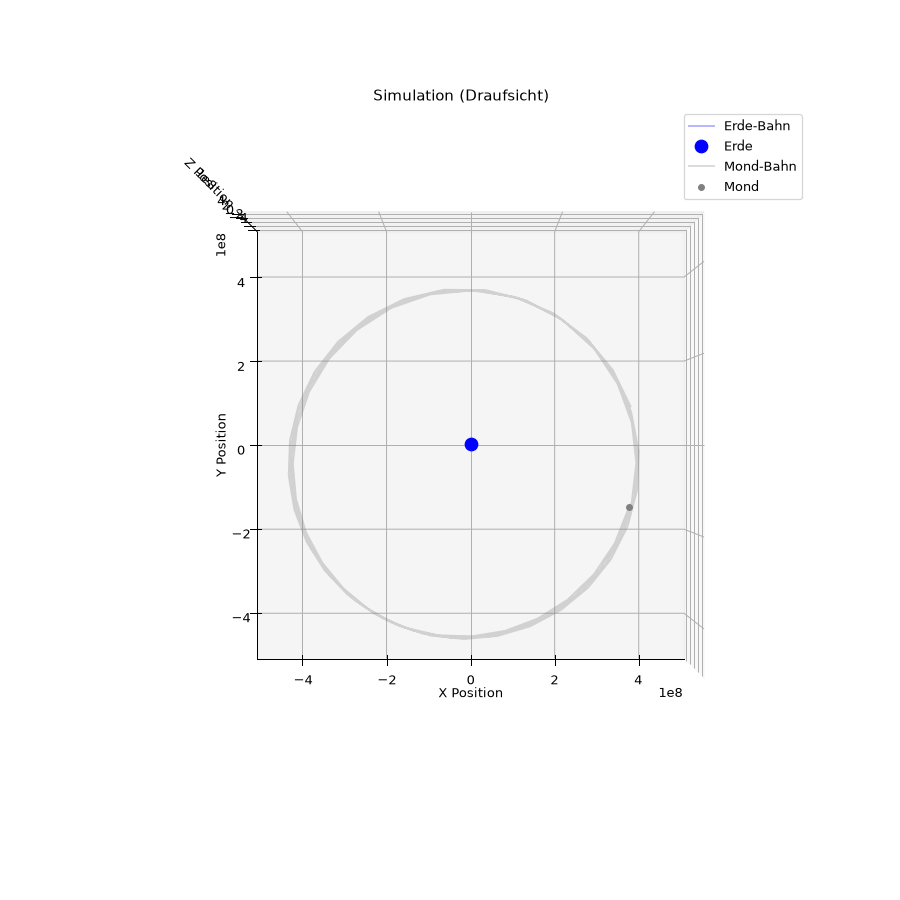
\includegraphics[keepaspectratio]{img/earth_moon_simulation.png}}
\caption{Bild}
\end{figure}

    \section{Theia-Physik}\label{theia-physik}


Für die Untersuchung der Kollisionshypothese und der Systemstabilität
unter dem Einfluss eines einfallenden, marsgroßen Protoplaneten (Theia)
\cite{quelle8} wurde die Klasse \texttt{scenario\_controller} implementiert.
Diese fungiert als Bindeglied zwischen den astronomischen
Anfangsbedingungen und der physikalischen Simulations-Engine.

\subsection{Mathematische Herleitung der variablen
Geometrie}\label{mathematische-herleitung-der-variablen-geometrie}

Zu beginn bilden Erde Mond und Theia ein gleichschenkliges Dreieck,
wobei Theia aus einer Distanz von \(4.000.000\,\text{km}\)
(\(4 \cdot 10^9\,\text{m}\)) in das System einfällt. Um die Simulation
maximal flexibel zu gestalten -- beispielsweise für eine zeitlich
verzögerte Injektion nach einer orbitalen Einschwingphase des
Erde-Mond-Systems --, wird die Startposition von Theia dynamisch aus den
\textbf{aktuellen Positionsvektoren} von Erde (\(\vec{p}_E\)) und Mond
(\(\vec{p}_M\)) abgeleitet.

\textbf{Berechnung der Systemmitte}

\[\vec{p}_{\text{mitte}} = \frac{\vec{p}_E + \vec{p}_M}{2}\]

\textbf{Orthogonaler Richtungsvektor}

Aus dem Verbindungsvektor
\(\vec{r}_{EM} = \vec{p}_M - \vec{p}_E = (x, y, 0)^T\) wird durch
Inversion und Permutation der Komponenten der Normalenvektor
\(\vec{n} = (-y, x, 0)^T\) konstruiert. Dieser steht im
\(90^\circ\)-Winkel auf der Erde-Mond-Achse.

\textbf{Normierung und Skalierung}

Der Normalenvektor wird auf die Länge \(1\,\text{m}\) normiert und mit
der Zielhöhe \(h = 4 \cdot 10^9\,\text{m}\) multipliziert:
\[\vec{p}_{\text{Theia}} = \vec{p}_{\text{mitte}} + \left( \frac{\vec{n}}{\|\vec{n}\|} \cdot h \right)\]

\subsection{Dynamische Richtungs- und
Impulsinitialisierung}\label{dynamische-richtungs--und-impulsinitialisierung}

Der initiale Geschwindigkeitsvektor \(\vec{v}_{\text{Theia}}\) wird
einmalig zum Injektionszeitpunkt berechnet. Je nach gewähltem
\texttt{target\_type} (``erde'', ``mond'' oder ``mitte'') wird der
Zielpunkt \(\vec{p}_{\text{ziel}}\) aus den aktuellen Positionen der
Simulation errechnet. Der resultierende Richtungsvektor wird normiert
und mit dem Betrag der geforderten Eintrittsgeschwindigkeit
(\(3\,\text{km/s}\), \(8\,\text{km/s}\) oder \(12\,\text{km/s}\))
skaliert.

    \begin{tcolorbox}[breakable, size=fbox, boxrule=1pt, pad at break*=1mm,colback=cellbackground, colframe=cellborder]
\prompt{In}{incolor}{ }{\boxspacing}
\begin{Verbatim}[commandchars=\\\{\}]
\PY{k+kn}{import}\PY{+w}{ }\PY{n+nn}{numpy}\PY{+w}{ }\PY{k}{as}\PY{+w}{ }\PY{n+nn}{np}

\PY{k}{class}\PY{+w}{ }\PY{n+nc}{ScenarioController}\PY{p}{:}
    \PY{k}{def}\PY{+w}{ }\PY{n+nf+fm}{\PYZus{}\PYZus{}init\PYZus{}\PYZus{}}\PY{p}{(}\PY{n+nb+bp}{self}\PY{p}{,} \PY{n}{speed\PYZus{}magnitude}\PY{p}{,} \PY{n}{target\PYZus{}type}\PY{p}{)}\PY{p}{:}
        \PY{n+nb+bp}{self}\PY{o}{.}\PY{n}{speed\PYZus{}magnitude} \PY{o}{=} \PY{n+nb}{float}\PY{p}{(}\PY{n}{speed\PYZus{}magnitude}\PY{p}{)}
        \PY{n+nb+bp}{self}\PY{o}{.}\PY{n}{target\PYZus{}type} \PY{o}{=} \PY{n}{target\PYZus{}type}\PY{o}{.}\PY{n}{lower}\PY{p}{(}\PY{p}{)}
        \PY{n+nb+bp}{self}\PY{o}{.}\PY{n}{distance} \PY{o}{=} \PY{l+m+mi}{4\PYZus{}000\PYZus{}000} \PY{o}{*} \PY{l+m+mi}{1000}  \PY{c+c1}{\PYZsh{} 4 Millonen km in Metern}
        
    \PY{k}{def}\PY{+w}{ }\PY{n+nf}{calculate\PYZus{}geometry}\PY{p}{(}\PY{n+nb+bp}{self}\PY{p}{,} \PY{n}{simulation}\PY{p}{)}\PY{p}{:}
\PY{+w}{        }\PY{l+s+sd}{\PYZdq{}\PYZdq{}\PYZdq{}}
\PY{l+s+sd}{        Berechnet die 3D\PYZhy{}Positionsvektoren für ein gleichschenkliges Dreieck,}
\PY{l+s+sd}{        basierend auf den aktuellen Positionen von Erde und Mond in der Simulation.}
\PY{l+s+sd}{        (Simulation kann also eine gewisse Zeit laufen, bis Theia hinzukommt)}
\PY{l+s+sd}{        }
\PY{l+s+sd}{        Returns:}
\PY{l+s+sd}{        \PYZhy{} theia\PYZus{}pos als np.ndarray}
\PY{l+s+sd}{        \PYZdq{}\PYZdq{}\PYZdq{}}
        
        \PY{c+c1}{\PYZsh{} 1. Erde und Mond aus der laufenden Simulation suchen}
        \PY{n}{erde\PYZus{}pos} \PY{o}{=} \PY{k+kc}{None}
        \PY{n}{mond\PYZus{}pos} \PY{o}{=} \PY{k+kc}{None}
        \PY{k}{for} \PY{n}{body} \PY{o+ow}{in} \PY{n}{simulation}\PY{o}{.}\PY{n}{bodies}\PY{p}{:}
            \PY{k}{if} \PY{l+s+s2}{\PYZdq{}}\PY{l+s+s2}{erde}\PY{l+s+s2}{\PYZdq{}} \PY{o+ow}{in} \PY{n}{body}\PY{o}{.}\PY{n}{name}\PY{o}{.}\PY{n}{lower}\PY{p}{(}\PY{p}{)}\PY{p}{:}
                \PY{n}{erde\PYZus{}pos} \PY{o}{=} \PY{n}{body}\PY{o}{.}\PY{n}{position}
            \PY{k}{elif} \PY{l+s+s2}{\PYZdq{}}\PY{l+s+s2}{mond}\PY{l+s+s2}{\PYZdq{}} \PY{o+ow}{in} \PY{n}{body}\PY{o}{.}\PY{n}{name}\PY{o}{.}\PY{n}{lower}\PY{p}{(}\PY{p}{)}\PY{p}{:}
                \PY{n}{mond\PYZus{}pos} \PY{o}{=} \PY{n}{body}\PY{o}{.}\PY{n}{position}
                
        \PY{k}{if} \PY{n}{erde\PYZus{}pos} \PY{o+ow}{is} \PY{k+kc}{None} \PY{o+ow}{or} \PY{n}{mond\PYZus{}pos} \PY{o+ow}{is} \PY{k+kc}{None}\PY{p}{:}
            \PY{k}{raise} \PY{n+ne}{ValueError}\PY{p}{(}\PY{l+s+s2}{\PYZdq{}}\PY{l+s+s2}{Erde oder Mond konnten für die Geometrie\PYZhy{}Berechnung nicht in der Simulation gefunden werden!}\PY{l+s+s2}{\PYZdq{}}\PY{p}{)}
            
        \PY{c+c1}{\PYZsh{} 2. Aktuellen Basis\PYZhy{}Vektor berechnen}
        \PY{n}{r\PYZus{}erde\PYZus{}mond} \PY{o}{=} \PY{n}{mond\PYZus{}pos} \PY{o}{\PYZhy{}} \PY{n}{erde\PYZus{}pos}  
        
        
        \PY{c+c1}{\PYZsh{} 3. Mittelpunkt zwischen Erde und Mond}
        \PY{n}{mitte\PYZus{}pos} \PY{o}{=} \PY{p}{(}\PY{n}{erde\PYZus{}pos} \PY{o}{+} \PY{n}{mond\PYZus{}pos}\PY{p}{)} \PY{o}{/} \PY{l+m+mf}{2.0}
        
        \PY{c+c1}{\PYZsh{} 4. Einen Vektor berechnen, der senkrecht auf der Erde\PYZhy{}Mond\PYZhy{}Linie steht (in der X/Y\PYZhy{}Ebene)}
        \PY{c+c1}{\PYZsh{} Wenn r\PYZus{}erde\PYZus{}mond = [x, y, 0], dann ist der senkrechte Vektor n = [\PYZhy{}y, x, 0]}
        \PY{n}{senkrecht\PYZus{}vektor} \PY{o}{=} \PY{n}{np}\PY{o}{.}\PY{n}{array}\PY{p}{(}\PY{p}{[}\PY{o}{\PYZhy{}}\PY{n}{r\PYZus{}erde\PYZus{}mond}\PY{p}{[}\PY{l+m+mi}{1}\PY{p}{]}\PY{p}{,} \PY{n}{r\PYZus{}erde\PYZus{}mond}\PY{p}{[}\PY{l+m+mi}{0}\PY{p}{]}\PY{p}{,} \PY{l+m+mf}{0.0}\PY{p}{]}\PY{p}{)}
        
        \PY{c+c1}{\PYZsh{} 5.auf die Länge 1 normieren}
        \PY{n}{senkrecht\PYZus{}normiert} \PY{o}{=} \PY{n}{senkrecht\PYZus{}vektor} \PY{o}{/} \PY{n}{np}\PY{o}{.}\PY{n}{linalg}\PY{o}{.}\PY{n}{norm}\PY{p}{(}\PY{n}{senkrecht\PYZus{}vektor}\PY{p}{)}
    
        
        \PY{c+c1}{\PYZsh{} 6. Theias Position ist: Mitte + (normierter Senkrechten\PYZhy{}Vektor * Distanz)}
        \PY{n}{theia\PYZus{}pos} \PY{o}{=} \PY{n}{mitte\PYZus{}pos} \PY{o}{+} \PY{p}{(}\PY{n}{senkrecht\PYZus{}normiert} \PY{o}{*} \PY{n+nb+bp}{self}\PY{o}{.}\PY{n}{distance}\PY{p}{)}
        
        \PY{k}{return} \PY{n}{theia\PYZus{}pos}

    \PY{k}{def}\PY{+w}{ }\PY{n+nf}{calculate\PYZus{}velocity\PYZus{}vector}\PY{p}{(}\PY{n+nb+bp}{self}\PY{p}{,} \PY{n}{start\PYZus{}pos}\PY{p}{:} \PY{n}{np}\PY{o}{.}\PY{n}{ndarray}\PY{p}{,} \PY{n}{target\PYZus{}type}\PY{p}{:} \PY{n+nb}{str}\PY{p}{,} \PY{n}{simulation}\PY{p}{)} \PY{o}{\PYZhy{}}\PY{o}{\PYZgt{}} \PY{n}{np}\PY{o}{.}\PY{n}{ndarray}\PY{p}{:}
\PY{+w}{        }\PY{l+s+sd}{\PYZdq{}\PYZdq{}\PYZdq{}}
\PY{l+s+sd}{        Bestimmt den präzisen, normierten Richtungsvektor vom Start\PYZhy{} zum }
\PY{l+s+sd}{        gewählten Zielpunkt und skaliert ihn mit der vorgegebenen Geschwindigkeit.}
\PY{l+s+sd}{        }
\PY{l+s+sd}{        Parameter:}
\PY{l+s+sd}{        \PYZhy{} start\PYZus{}pos: Die 3D\PYZhy{}Startposition von Theia [x, y, z]}
\PY{l+s+sd}{        \PYZhy{} target\PYZus{}type: Der Typ des Ziels (erde, mond, mitte)}
\PY{l+s+sd}{        \PYZhy{} simulation: Die laufende Simulation}
\PY{l+s+sd}{        }
\PY{l+s+sd}{        Returns:}
\PY{l+s+sd}{        \PYZhy{} Ein 3D\PYZhy{}NumPy\PYZhy{}Array, das den initialen Geschwindigkeitsvektor darstellt.}
\PY{l+s+sd}{        \PYZdq{}\PYZdq{}\PYZdq{}}
        \PY{n}{target\PYZus{}type\PYZus{}clean} \PY{o}{=} \PY{n}{target\PYZus{}type}\PY{o}{.}\PY{n}{lower}\PY{p}{(}\PY{p}{)}
        \PY{n}{erde\PYZus{}pos} \PY{o}{=} \PY{k+kc}{None}
        \PY{n}{mond\PYZus{}pos} \PY{o}{=} \PY{k+kc}{None}
        
        \PY{c+c1}{\PYZsh{} Aktuelle Positionen}
        \PY{k}{for} \PY{n}{body} \PY{o+ow}{in} \PY{n}{simulation}\PY{o}{.}\PY{n}{bodies}\PY{p}{:}
            \PY{k}{if} \PY{l+s+s2}{\PYZdq{}}\PY{l+s+s2}{erde}\PY{l+s+s2}{\PYZdq{}} \PY{o+ow}{in} \PY{n}{body}\PY{o}{.}\PY{n}{name}\PY{o}{.}\PY{n}{lower}\PY{p}{(}\PY{p}{)}\PY{p}{:}
                \PY{n}{erde\PYZus{}pos} \PY{o}{=} \PY{n}{body}\PY{o}{.}\PY{n}{position}
            \PY{k}{elif} \PY{l+s+s2}{\PYZdq{}}\PY{l+s+s2}{mond}\PY{l+s+s2}{\PYZdq{}} \PY{o+ow}{in} \PY{n}{body}\PY{o}{.}\PY{n}{name}\PY{o}{.}\PY{n}{lower}\PY{p}{(}\PY{p}{)}\PY{p}{:}
                \PY{n}{mond\PYZus{}pos} \PY{o}{=} \PY{n}{body}\PY{o}{.}\PY{n}{position}

        \PY{c+c1}{\PYZsh{} Zielposition basierend auf dem Zieltyp bestimmen}
        \PY{k}{if} \PY{n}{erde\PYZus{}pos} \PY{o+ow}{is} \PY{k+kc}{None} \PY{o+ow}{or} \PY{n}{mond\PYZus{}pos} \PY{o+ow}{is} \PY{k+kc}{None}\PY{p}{:} 
                \PY{k}{raise} \PY{n+ne}{ValueError}\PY{p}{(}\PY{l+s+s2}{\PYZdq{}}\PY{l+s+s2}{Erde oder Mond konnten nicht gefunden werden!}\PY{l+s+s2}{\PYZdq{}}\PY{p}{)}
            
        \PY{k}{if} \PY{n}{target\PYZus{}type\PYZus{}clean} \PY{o}{==} \PY{l+s+s2}{\PYZdq{}}\PY{l+s+s2}{erde}\PY{l+s+s2}{\PYZdq{}}\PY{p}{:}
            \PY{n}{target\PYZus{}pos} \PY{o}{=} \PY{n}{erde\PYZus{}pos}
            
        \PY{k}{elif} \PY{n}{target\PYZus{}type\PYZus{}clean} \PY{o}{==} \PY{l+s+s2}{\PYZdq{}}\PY{l+s+s2}{mond}\PY{l+s+s2}{\PYZdq{}}\PY{p}{:}
            \PY{n}{target\PYZus{}pos} \PY{o}{=} \PY{n}{mond\PYZus{}pos}
            
        \PY{k}{elif} \PY{n}{target\PYZus{}type\PYZus{}clean} \PY{o}{==} \PY{l+s+s2}{\PYZdq{}}\PY{l+s+s2}{mitte}\PY{l+s+s2}{\PYZdq{}}\PY{p}{:}
            \PY{n}{target\PYZus{}pos} \PY{o}{=} \PY{p}{(}\PY{n}{erde\PYZus{}pos} \PY{o}{+} \PY{n}{mond\PYZus{}pos}\PY{p}{)} \PY{o}{/} \PY{l+m+mf}{2.0}
            
        \PY{k}{else}\PY{p}{:}
            \PY{k}{raise} \PY{n+ne}{ValueError}\PY{p}{(}\PY{l+s+s2}{\PYZdq{}}\PY{l+s+s2}{Ungültiger Zieltyp! Verwenden Sie }\PY{l+s+s2}{\PYZsq{}}\PY{l+s+s2}{erde}\PY{l+s+s2}{\PYZsq{}}\PY{l+s+s2}{, }\PY{l+s+s2}{\PYZsq{}}\PY{l+s+s2}{mond}\PY{l+s+s2}{\PYZsq{}}\PY{l+s+s2}{ oder }\PY{l+s+s2}{\PYZsq{}}\PY{l+s+s2}{mitte}\PY{l+s+s2}{\PYZsq{}}\PY{l+s+s2}{.}\PY{l+s+s2}{\PYZdq{}}\PY{p}{)}

        \PY{c+c1}{\PYZsh{} Vektor von Theia zum Ziel berechnen}
        \PY{n}{direction} \PY{o}{=} \PY{n}{target\PYZus{}pos} \PY{o}{\PYZhy{}} \PY{n}{start\PYZus{}pos}
        
        \PY{c+c1}{\PYZsh{} Die Länge des Richtungsvektors (Abstand) berechnen}
        \PY{n}{distance} \PY{o}{=} \PY{n}{np}\PY{o}{.}\PY{n}{linalg}\PY{o}{.}\PY{n}{norm}\PY{p}{(}\PY{n}{direction}\PY{p}{)}
        
        \PY{k}{if} \PY{n}{distance} \PY{o}{==} \PY{l+m+mi}{0}\PY{p}{:}
            \PY{k}{raise} \PY{n+ne}{ValueError}\PY{p}{(}\PY{l+s+s2}{\PYZdq{}}\PY{l+s+s2}{Start\PYZhy{} und Zielposition sind identisch! Division durch Null verhindert.}\PY{l+s+s2}{\PYZdq{}}\PY{p}{)}
            
        \PY{c+c1}{\PYZsh{} Vektor normieren (auf die Länge 1 bringen)}
        \PY{n}{direction\PYZus{}normed} \PY{o}{=} \PY{n}{direction} \PY{o}{/} \PY{n}{distance}
        
        \PY{c+c1}{\PYZsh{} Mit dem Betrag der Geschwindigkeit multiplizieren, um v\PYZus{}x, v\PYZus{}y, v\PYZus{}z zu erhalten}
        \PY{n}{velocity\PYZus{}vector} \PY{o}{=} \PY{n}{direction\PYZus{}normed} \PY{o}{*} \PY{n+nb+bp}{self}\PY{o}{.}\PY{n}{speed\PYZus{}magnitude}
        
        \PY{k}{return} \PY{n}{velocity\PYZus{}vector}
    
    \PY{k}{def}\PY{+w}{ }\PY{n+nf}{setup\PYZus{}theia}\PY{p}{(}\PY{n+nb+bp}{self}\PY{p}{,} \PY{n}{simulation}\PY{p}{)}\PY{p}{:}
\PY{+w}{        }\PY{l+s+sd}{\PYZdq{}\PYZdq{}\PYZdq{}}
\PY{l+s+sd}{        Berechnet die Startwerte für Theia und fügt sie direkt der Simulation hinzu.}
\PY{l+s+sd}{        \PYZdq{}\PYZdq{}\PYZdq{}}
        \PY{c+c1}{\PYZsh{} 1. Startposition über die Geometrie holen}
        \PY{n}{theia\PYZus{}start\PYZus{}pos} \PY{o}{=} \PY{n+nb+bp}{self}\PY{o}{.}\PY{n}{calculate\PYZus{}geometry}\PY{p}{(}\PY{n}{simulation}\PY{p}{)}
        
        \PY{c+c1}{\PYZsh{} 2. Anfangsgeschwindigkeitsvektor berechnen}
        \PY{n}{theia\PYZus{}velocity} \PY{o}{=} \PY{n+nb+bp}{self}\PY{o}{.}\PY{n}{calculate\PYZus{}velocity\PYZus{}vector}\PY{p}{(}\PY{n}{theia\PYZus{}start\PYZus{}pos}\PY{p}{,} \PY{n+nb+bp}{self}\PY{o}{.}\PY{n}{target\PYZus{}type}\PY{p}{,} \PY{n}{simulation}\PY{p}{)}
        
        \PY{c+c1}{\PYZsh{} 3. Theia\PYZhy{}Body\PYZhy{}Objekt erstellen und injizieren}
        \PY{n}{theia} \PY{o}{=} \PY{n}{Body}\PY{p}{(}\PY{l+s+s2}{\PYZdq{}}\PY{l+s+s2}{Theia}\PY{l+s+s2}{\PYZdq{}}\PY{p}{,} \PY{n}{theia\PYZus{}start\PYZus{}pos}\PY{p}{,} \PY{n}{theia\PYZus{}velocity}\PY{p}{,} \PY{l+m+mf}{3389000.0}\PY{p}{,} \PY{l+m+mf}{6.39e23}\PY{p}{,} \PY{l+s+s2}{\PYZdq{}}\PY{l+s+s2}{red}\PY{l+s+s2}{\PYZdq{}}\PY{p}{)} \PY{c+c1}{\PYZsh{} Radius und Masse konstant wie Mars}
        \PY{n}{simulation}\PY{o}{.}\PY{n}{add\PYZus{}body}\PY{p}{(}\PY{n}{theia}\PY{p}{)}
        
        \PY{n+nb}{print}\PY{p}{(}\PY{l+s+sa}{f}\PY{l+s+s2}{\PYZdq{}}\PY{l+s+s2}{Theia erfolgreich Richtung }\PY{l+s+s2}{\PYZsq{}}\PY{l+s+si}{\PYZob{}}\PY{n+nb+bp}{self}\PY{o}{.}\PY{n}{target\PYZus{}type}\PY{l+s+si}{\PYZcb{}}\PY{l+s+s2}{\PYZsq{}}\PY{l+s+s2}{ injiziert.}\PY{l+s+s2}{\PYZdq{}}\PY{p}{)}
\end{Verbatim}
\end{tcolorbox}

    \section{Auswertung:
Theia-Szenarien}\label{auswertung-theia-szenarien}

In diesem Experiment simulieren wir den Einschlag eines marsgroßen
Himmelskörpers (Theia) in das Erde-Mond-System aus 4 Millionen
Kilometern Entfernung. Das greift die \emph{Giant-Impact-Hypothese} auf,
nach der unser Mond aus der Kollision der jungen Erde mit einem solchen
Körper hervorgegangen sein soll.

Um die Systemstabilität zu untersuchen, variieren wir die Parameter
systematisch: - \textbf{Anfangsgeschwindigkeit:} 3 km/s, 8 km/s und 12
km/s. - \textbf{Zielrichtung:} Exakt auf die \textbf{Erde}, den
\textbf{Mond} oder die \textbf{Mitte} zwischen beiden.

\textbf{Leitfrage}

Gibt es unter den getesteten Konfigurationen eine, bei der es zu keiner
Kollision kommt?

\textbf{Hinweis zur Numerik (Tunnel-Effekt)}

Bei hohen Geschwindigkeiten legt Theia pro Zeitschritt große Strecken
zurück. Bei 12~km/s sind das rund 2.000~km pro Zeitschritt -- deutlich
weniger als der ca. 9.760~km breite Kollisionskorridor (Summe der Radien
von Erde und Theia). So wird verhindert, dass Theia in einem einzigen
Berechnungssprung durch einen Körper „hindurchtunnelt``, ohne dass die
Kollisionserkennung greift. Die Simulation läuft dafür mit einem kleinen
Zeitschritt von 0.002 Tagen (ca. 173~s).

Der folgende automatisierte Testlauf spielt alle 9 Basis-Kombinationen
durch. Er erzeugt eine Ergebnistabelle, plottet anschließend den
\textbf{Abstandsverlauf Theia--Erde} für alle Szenarien und visualisiert
abschließend je ein repräsentatives Kollisions- und Vorbeiflug-Szenario
in 3D.

    \begin{tcolorbox}[breakable, size=fbox, boxrule=1pt, pad at break*=1mm,colback=cellbackground, colframe=cellborder]
\prompt{In}{incolor}{51}{\boxspacing}
\begin{Verbatim}[commandchars=\\\{\}]
\PY{c+c1}{\PYZsh{} ============================================================================}
\PY{c+c1}{\PYZsh{} Erst Hilfsfunktionen, dann 3x3 = 9 Szenarien, am Ende eine Ergebnistabelle.}
\PY{c+c1}{\PYZsh{} ============================================================================}

\PY{c+c1}{\PYZsh{} numpy stellt Vektor\PYZhy{}/Array\PYZhy{}Rechnung bereit (Positionen, Abstaende, np.inf usw.).}
\PY{k+kn}{import}\PY{+w}{ }\PY{n+nn}{numpy}\PY{+w}{ }\PY{k}{as}\PY{+w}{ }\PY{n+nn}{np}

\PY{n}{KM\PYZus{}PER\PYZus{}S\PYZus{}TO\PYZus{}M\PYZus{}PER\PYZus{}DAY} \PY{o}{=} \PY{l+m+mi}{1000} \PY{o}{*} \PY{l+m+mi}{86400}


\PY{k}{def}\PY{+w}{ }\PY{n+nf}{baue\PYZus{}erde\PYZus{}mond\PYZus{}sim}\PY{p}{(}\PY{n}{time\PYZus{}step}\PY{p}{)}\PY{p}{:}
\PY{+w}{    }\PY{l+s+sd}{\PYZdq{}\PYZdq{}\PYZdq{}Baut eine frische Simulation mit Erde (ruhend) und Mond (auf Kreisbahn).\PYZdq{}\PYZdq{}\PYZdq{}}

    \PY{c+c1}{\PYZsh{} Neue, leere Simulation mit dem gewuenschten Zeitschritt anlegen.}
    \PY{n}{sim} \PY{o}{=} \PY{n}{Simulation}\PY{p}{(}\PY{n}{time\PYZus{}step}\PY{p}{)}
    \PY{c+c1}{\PYZsh{}Position, Radius, Masse}
    \PY{n}{sim}\PY{o}{.}\PY{n}{add\PYZus{}body}\PY{p}{(}\PY{n}{Body}\PY{p}{(}\PY{l+s+s2}{\PYZdq{}}\PY{l+s+s2}{Erde}\PY{l+s+s2}{\PYZdq{}}\PY{p}{,} \PY{p}{[}\PY{l+m+mi}{0}\PY{p}{,} \PY{l+m+mi}{0}\PY{p}{,} \PY{l+m+mi}{0}\PY{p}{]}\PY{p}{,}         \PY{p}{[}\PY{l+m+mi}{0}\PY{p}{,} \PY{o}{\PYZhy{}}\PY{l+m+mf}{12.573} \PY{o}{*} \PY{l+m+mi}{86400}\PY{p}{,} \PY{l+m+mi}{0}\PY{p}{]}\PY{p}{,} \PY{l+m+mi}{6371000}\PY{p}{,} \PY{l+m+mf}{5.972e24}\PY{p}{,} \PY{l+s+s2}{\PYZdq{}}\PY{l+s+s2}{blue}\PY{l+s+s2}{\PYZdq{}}\PY{p}{)}\PY{p}{)}
    \PY{n}{sim}\PY{o}{.}\PY{n}{add\PYZus{}body}\PY{p}{(}\PY{n}{Body}\PY{p}{(}\PY{l+s+s2}{\PYZdq{}}\PY{l+s+s2}{Mond}\PY{l+s+s2}{\PYZdq{}}\PY{p}{,} \PY{p}{[}\PY{l+m+mi}{384400000}\PY{p}{,} \PY{l+m+mi}{0}\PY{p}{,} \PY{l+m+mi}{0}\PY{p}{]}\PY{p}{,} \PY{p}{[}\PY{l+m+mi}{0}\PY{p}{,}  \PY{l+m+mi}{1022}   \PY{o}{*} \PY{l+m+mi}{86400}\PY{p}{,} \PY{l+m+mi}{0}\PY{p}{]}\PY{p}{,} \PY{l+m+mi}{1737000}\PY{p}{,} \PY{l+m+mf}{7.348e22}\PY{p}{,} \PY{l+s+s2}{\PYZdq{}}\PY{l+s+s2}{grey}\PY{l+s+s2}{\PYZdq{}}\PY{p}{)}\PY{p}{)}

    \PY{k}{return} \PY{n}{sim}


\PY{k}{def}\PY{+w}{ }\PY{n+nf}{\PYZus{}abstand\PYZus{}verlauf}\PY{p}{(}\PY{n}{sim}\PY{p}{,} \PY{n}{name\PYZus{}a}\PY{p}{,} \PY{n}{name\PYZus{}b}\PY{p}{)}\PY{p}{:}
\PY{+w}{    }\PY{l+s+sd}{\PYZdq{}\PYZdq{}\PYZdq{}Liefert den zeitlichen Abstand zweier Koerper als (tage, abstand\PYZus{}in\PYZus{}km).\PYZdq{}\PYZdq{}\PYZdq{}}

    \PY{c+c1}{\PYZsh{} Gespeicherte Positionen von Koerper A aus der history holen und in ein float\PYZhy{}Array packen.}
    \PY{n}{ha} \PY{o}{=} \PY{n}{np}\PY{o}{.}\PY{n}{array}\PY{p}{(}\PY{n}{sim}\PY{o}{.}\PY{n}{history}\PY{o}{.}\PY{n}{get}\PY{p}{(}\PY{n}{name\PYZus{}a}\PY{p}{,} \PY{p}{[}\PY{p}{]}\PY{p}{)}\PY{p}{,} \PY{n}{dtype}\PY{o}{=}\PY{n+nb}{float}\PY{p}{)}
    \PY{n}{hb} \PY{o}{=} \PY{n}{np}\PY{o}{.}\PY{n}{array}\PY{p}{(}\PY{n}{sim}\PY{o}{.}\PY{n}{history}\PY{o}{.}\PY{n}{get}\PY{p}{(}\PY{n}{name\PYZus{}b}\PY{p}{,} \PY{p}{[}\PY{p}{]}\PY{p}{)}\PY{p}{,} \PY{n}{dtype}\PY{o}{=}\PY{n+nb}{float}\PY{p}{)}
    \PY{k}{if} \PY{n}{ha}\PY{o}{.}\PY{n}{size} \PY{o}{==} \PY{l+m+mi}{0} \PY{o+ow}{or} \PY{n}{hb}\PY{o}{.}\PY{n}{size} \PY{o}{==} \PY{l+m+mi}{0}\PY{p}{:}
        \PY{k}{return} \PY{n}{np}\PY{o}{.}\PY{n}{array}\PY{p}{(}\PY{p}{[}\PY{p}{]}\PY{p}{)}\PY{p}{,} \PY{n}{np}\PY{o}{.}\PY{n}{array}\PY{p}{(}\PY{p}{[}\PY{p}{]}\PY{p}{)}

    \PY{c+c1}{\PYZsh{} Beide Verlaeufe auf die gleiche (kuerzere) Laenge bringen, damit sie zusammenpassen.}
    \PY{n}{n} \PY{o}{=} \PY{n+nb}{min}\PY{p}{(}\PY{n+nb}{len}\PY{p}{(}\PY{n}{ha}\PY{p}{)}\PY{p}{,} \PY{n+nb}{len}\PY{p}{(}\PY{n}{hb}\PY{p}{)}\PY{p}{)}

    \PY{c+c1}{\PYZsh{} (Index * Zeitschritt).}
    \PY{n}{tage} \PY{o}{=} \PY{n}{np}\PY{o}{.}\PY{n}{arange}\PY{p}{(}\PY{n}{n}\PY{p}{)} \PY{o}{*} \PY{n}{sim}\PY{o}{.}\PY{n}{time\PYZus{}step}

    \PY{c+c1}{\PYZsh{} Pro Zeitschritt den Abstand berechnen (Betrag der Differenzvektoren) und in km umrechnen.}
    \PY{n}{dist} \PY{o}{=} \PY{n}{np}\PY{o}{.}\PY{n}{linalg}\PY{o}{.}\PY{n}{norm}\PY{p}{(}\PY{n}{ha}\PY{p}{[}\PY{p}{:}\PY{n}{n}\PY{p}{]} \PY{o}{\PYZhy{}} \PY{n}{hb}\PY{p}{[}\PY{p}{:}\PY{n}{n}\PY{p}{]}\PY{p}{,} \PY{n}{axis}\PY{o}{=}\PY{l+m+mi}{1}\PY{p}{)} \PY{o}{/} \PY{l+m+mi}{1000}

    \PY{k}{return} \PY{n}{tage}\PY{p}{,} \PY{n}{dist}


\PY{k}{def}\PY{+w}{ }\PY{n+nf}{finde\PYZus{}koerper}\PY{p}{(}\PY{n}{sim}\PY{p}{,} \PY{n}{name}\PY{p}{)}\PY{p}{:}
\PY{+w}{    }\PY{l+s+sd}{\PYZdq{}\PYZdq{}\PYZdq{}Sucht den lebenden Koerper mit genau diesem Namen; gibt None zurueck, wenn es ihn nicht (mehr) gibt.\PYZdq{}\PYZdq{}\PYZdq{}}

    \PY{k}{for} \PY{n}{b} \PY{o+ow}{in} \PY{n}{sim}\PY{o}{.}\PY{n}{bodies}\PY{p}{:}
        \PY{k}{if} \PY{n}{b}\PY{o}{.}\PY{n}{name} \PY{o}{==} \PY{n}{name}\PY{p}{:}
            \PY{k}{return} \PY{n}{b}
    \PY{k}{return} \PY{k+kc}{None}


\PY{k}{def}\PY{+w}{ }\PY{n+nf}{run\PYZus{}theia\PYZus{}scenario}\PY{p}{(}\PY{n}{speed\PYZus{}kms}\PY{p}{,} \PY{n}{target}\PY{p}{,} \PY{n}{total\PYZus{}time}\PY{o}{=}\PY{l+m+mi}{30}\PY{p}{,} \PY{n}{time\PYZus{}step}\PY{o}{=}\PY{l+m+mf}{0.002}\PY{p}{)}\PY{p}{:}
\PY{+w}{    }\PY{l+s+sd}{\PYZdq{}\PYZdq{}\PYZdq{}Baut Erde+Mond, schiesst Theia hinein und laesst das System laufen. Returns (sim, ergebnis\PYZhy{}dict).\PYZdq{}\PYZdq{}\PYZdq{}}

    \PY{n}{sim} \PY{o}{=} \PY{n}{baue\PYZus{}erde\PYZus{}mond\PYZus{}sim}\PY{p}{(}\PY{n}{time\PYZus{}step}\PY{p}{)}

    \PY{n}{controller} \PY{o}{=} \PY{n}{ScenarioController}\PY{p}{(}
        \PY{n}{speed\PYZus{}magnitude}\PY{o}{=}\PY{n}{speed\PYZus{}kms} \PY{o}{*} \PY{n}{KM\PYZus{}PER\PYZus{}S\PYZus{}TO\PYZus{}M\PYZus{}PER\PYZus{}DAY}\PY{p}{,}
        \PY{n}{target\PYZus{}type}\PY{o}{=}\PY{n}{target}
    \PY{p}{)}

    \PY{n}{controller}\PY{o}{.}\PY{n}{setup\PYZus{}theia}\PY{p}{(}\PY{n}{sim}\PY{p}{)}
    \PY{n}{steps} \PY{o}{=} \PY{n+nb}{int}\PY{p}{(}\PY{n}{total\PYZus{}time} \PY{o}{/} \PY{n}{time\PYZus{}step}\PY{p}{)}
    \PY{n}{anzahl\PYZus{}koerper} \PY{o}{=} \PY{n+nb}{len}\PY{p}{(}\PY{n}{sim}\PY{o}{.}\PY{n}{bodies}\PY{p}{)}
    \PY{n}{kollisions\PYZus{}tag} \PY{o}{=} \PY{k+kc}{None}

    \PY{c+c1}{\PYZsh{} mit Unendlich starten, damit das erste min() greift.}
    \PY{n}{min\PYZus{}abstand\PYZus{}erde} \PY{o}{=} \PY{n}{np}\PY{o}{.}\PY{n}{inf}
    \PY{n}{min\PYZus{}abstand\PYZus{}mond} \PY{o}{=} \PY{n}{np}\PY{o}{.}\PY{n}{inf}

    \PY{c+c1}{\PYZsh{} Simulation Schritt fuer Schritt vorwaerts rechnen.}
    \PY{k}{for} \PY{n}{i} \PY{o+ow}{in} \PY{n+nb}{range}\PY{p}{(}\PY{n}{steps}\PY{p}{)}\PY{p}{:}

        \PY{n}{sim}\PY{o}{.}\PY{n}{step}\PY{p}{(}\PY{p}{)}
        \PY{n}{theia} \PY{o}{=} \PY{n}{finde\PYZus{}koerper}\PY{p}{(}\PY{n}{sim}\PY{p}{,} \PY{l+s+s2}{\PYZdq{}}\PY{l+s+s2}{Theia}\PY{l+s+s2}{\PYZdq{}}\PY{p}{)}

        \PY{c+c1}{\PYZsh{} Nur wenn Theia noch getrennt existiert}
        \PY{k}{if} \PY{n}{theia} \PY{o+ow}{is} \PY{o+ow}{not} \PY{k+kc}{None}\PY{p}{:}

            \PY{c+c1}{\PYZsh{} Erde und Mond als eigenen Koerper suchen.}
            \PY{n}{erde} \PY{o}{=} \PY{n}{finde\PYZus{}koerper}\PY{p}{(}\PY{n}{sim}\PY{p}{,} \PY{l+s+s2}{\PYZdq{}}\PY{l+s+s2}{Erde}\PY{l+s+s2}{\PYZdq{}}\PY{p}{)}
            \PY{n}{mond} \PY{o}{=} \PY{n}{finde\PYZus{}koerper}\PY{p}{(}\PY{n}{sim}\PY{p}{,} \PY{l+s+s2}{\PYZdq{}}\PY{l+s+s2}{Mond}\PY{l+s+s2}{\PYZdq{}}\PY{p}{)}

            \PY{c+c1}{\PYZsh{} kleinsten Abstand Theia\PYZhy{}Erde und Theia\PYZhy{}Mond aktualisieren.}
            \PY{k}{if} \PY{n}{erde} \PY{o+ow}{is} \PY{o+ow}{not} \PY{k+kc}{None}\PY{p}{:}
                \PY{n}{min\PYZus{}abstand\PYZus{}erde} \PY{o}{=} \PY{n+nb}{min}\PY{p}{(}\PY{n}{min\PYZus{}abstand\PYZus{}erde}\PY{p}{,} \PY{n}{theia}\PY{o}{.}\PY{n}{get\PYZus{}distance\PYZus{}to\PYZus{}body}\PY{p}{(}\PY{n}{erde}\PY{p}{)}\PY{p}{)}
            \PY{k}{if} \PY{n}{mond} \PY{o+ow}{is} \PY{o+ow}{not} \PY{k+kc}{None}\PY{p}{:}
                \PY{n}{min\PYZus{}abstand\PYZus{}mond} \PY{o}{=} \PY{n+nb}{min}\PY{p}{(}\PY{n}{min\PYZus{}abstand\PYZus{}mond}\PY{p}{,} \PY{n}{theia}\PY{o}{.}\PY{n}{get\PYZus{}distance\PYZus{}to\PYZus{}body}\PY{p}{(}\PY{n}{mond}\PY{p}{)}\PY{p}{)}

        \PY{c+c1}{\PYZsh{} Sind es weniger Koerper als vorher \PYZhy{}\PYZgt{} eine Verschmelzung hat stattgefunden.}
        \PY{c+c1}{\PYZsh{} Den Kollisionstag nur beim ersten Mal setzen: Schrittnummer * Zeitschritt = Tag.}
        \PY{k}{if} \PY{n}{kollisions\PYZus{}tag} \PY{o+ow}{is} \PY{k+kc}{None} \PY{o+ow}{and} \PY{n+nb}{len}\PY{p}{(}\PY{n}{sim}\PY{o}{.}\PY{n}{bodies}\PY{p}{)} \PY{o}{\PYZlt{}} \PY{n}{anzahl\PYZus{}koerper}\PY{p}{:}
            \PY{n}{kollisions\PYZus{}tag} \PY{o}{=} \PY{p}{(}\PY{n}{i} \PY{o}{+} \PY{l+m+mi}{1}\PY{p}{)} \PY{o}{*} \PY{n}{time\PYZus{}step}

        \PY{c+c1}{\PYZsh{} Koerperzahl fuer den Vergleich im naechsten Schritt aktualisieren.}
        \PY{n}{anzahl\PYZus{}koerper} \PY{o}{=} \PY{n+nb}{len}\PY{p}{(}\PY{n}{sim}\PY{o}{.}\PY{n}{bodies}\PY{p}{)}

    \PY{c+c1}{\PYZsh{} Nach dem Lauf herausfinden, mit wem Theia verschmolzen ist.}
    \PY{n}{kollision\PYZus{}mit} \PY{o}{=} \PY{k+kc}{None}

    \PY{c+c1}{\PYZsh{} Alle noch lebenden Koerper durchgehen.}
    \PY{k}{for} \PY{n}{b} \PY{o+ow}{in} \PY{n}{sim}\PY{o}{.}\PY{n}{bodies}\PY{p}{:}

        \PY{n}{teile} \PY{o}{=} \PY{n}{b}\PY{o}{.}\PY{n}{name}\PY{o}{.}\PY{n}{split}\PY{p}{(}\PY{l+s+s2}{\PYZdq{}}\PY{l+s+s2}{+}\PY{l+s+s2}{\PYZdq{}}\PY{p}{)}

        \PY{c+c1}{\PYZsh{} Steckt \PYZdq{}Theia\PYZdq{} im Namen UND noch etwas anderes, ist das der getroffene Koerper.}
        \PY{k}{if} \PY{l+s+s2}{\PYZdq{}}\PY{l+s+s2}{Theia}\PY{l+s+s2}{\PYZdq{}} \PY{o+ow}{in} \PY{n}{teile} \PY{o+ow}{and} \PY{n+nb}{len}\PY{p}{(}\PY{n}{teile}\PY{p}{)} \PY{o}{\PYZgt{}} \PY{l+m+mi}{1}\PY{p}{:}
            \PY{c+c1}{\PYZsh{} Die restlichen Namensteile verbinden z.B. \PYZdq{}Erde\PYZdq{} oder \PYZdq{}Erde+Mond\PYZdq{} (ohne Theia)}
            \PY{n}{kollision\PYZus{}mit} \PY{o}{=} \PY{l+s+s2}{\PYZdq{}}\PY{l+s+s2}{+}\PY{l+s+s2}{\PYZdq{}}\PY{o}{.}\PY{n}{join}\PY{p}{(}\PY{n}{t} \PY{k}{for} \PY{n}{t} \PY{o+ow}{in} \PY{n}{teile} \PY{k}{if} \PY{n}{t} \PY{o}{!=} \PY{l+s+s2}{\PYZdq{}}\PY{l+s+s2}{Theia}\PY{l+s+s2}{\PYZdq{}}\PY{p}{)}

    \PY{c+c1}{\PYZsh{} Gab es keine Verschmelzung, gibt es auch keinen Kollisionstag.}
    \PY{k}{if} \PY{n}{kollision\PYZus{}mit} \PY{o+ow}{is} \PY{k+kc}{None}\PY{p}{:}
        \PY{n}{kollisions\PYZus{}tag} \PY{o}{=} \PY{k+kc}{None}


    \PY{n}{ergebnis} \PY{o}{=} \PY{p}{\PYZob{}}
        \PY{l+s+s2}{\PYZdq{}}\PY{l+s+s2}{speed\PYZus{}kms}\PY{l+s+s2}{\PYZdq{}}\PY{p}{:}        \PY{n}{speed\PYZus{}kms}\PY{p}{,}        
        \PY{l+s+s2}{\PYZdq{}}\PY{l+s+s2}{target}\PY{l+s+s2}{\PYZdq{}}\PY{p}{:}           \PY{n}{target}\PY{p}{,}          
        \PY{l+s+s2}{\PYZdq{}}\PY{l+s+s2}{kollision\PYZus{}mit}\PY{l+s+s2}{\PYZdq{}}\PY{p}{:}    \PY{n}{kollision\PYZus{}mit}\PY{p}{,}    
        \PY{l+s+s2}{\PYZdq{}}\PY{l+s+s2}{kollisions\PYZus{}tag}\PY{l+s+s2}{\PYZdq{}}\PY{p}{:}   \PY{n}{kollisions\PYZus{}tag}\PY{p}{,}    
        \PY{l+s+s2}{\PYZdq{}}\PY{l+s+s2}{min\PYZus{}abstand\PYZus{}erde}\PY{l+s+s2}{\PYZdq{}}\PY{p}{:} \PY{n}{min\PYZus{}abstand\PYZus{}erde}\PY{p}{,}  
        \PY{l+s+s2}{\PYZdq{}}\PY{l+s+s2}{min\PYZus{}abstand\PYZus{}mond}\PY{l+s+s2}{\PYZdq{}}\PY{p}{:} \PY{n}{min\PYZus{}abstand\PYZus{}mond}\PY{p}{,}  
    \PY{p}{\PYZcb{}}

    \PY{k}{return} \PY{n}{sim}\PY{p}{,} \PY{n}{ergebnis}


\PY{n}{speeds}  \PY{o}{=} \PY{p}{[}\PY{l+m+mi}{3}\PY{p}{,} \PY{l+m+mi}{8}\PY{p}{,} \PY{l+m+mi}{12}\PY{p}{]}                    \PY{c+c1}{\PYZsh{}v}
\PY{n}{targets} \PY{o}{=} \PY{p}{[}\PY{l+s+s2}{\PYZdq{}}\PY{l+s+s2}{mitte}\PY{l+s+s2}{\PYZdq{}}\PY{p}{,} \PY{l+s+s2}{\PYZdq{}}\PY{l+s+s2}{mond}\PY{l+s+s2}{\PYZdq{}}\PY{p}{,} \PY{l+s+s2}{\PYZdq{}}\PY{l+s+s2}{erde}\PY{l+s+s2}{\PYZdq{}}\PY{p}{]}     \PY{c+c1}{\PYZsh{}t}

\PY{n}{ergebnisse}\PY{p}{,} \PY{n}{sims} \PY{o}{=} \PY{p}{[}\PY{p}{]}\PY{p}{,} \PY{p}{\PYZob{}}\PY{p}{\PYZcb{}}

\PY{n+nb}{print}\PY{p}{(}\PY{l+s+s2}{\PYZdq{}}\PY{l+s+s2}{Starte 9 Simulationen (3 Geschwindigkeiten x 3 Richtungen)...}\PY{l+s+se}{\PYZbs{}n}\PY{l+s+s2}{\PYZdq{}}\PY{p}{)}

\PY{k}{for} \PY{n}{v} \PY{o+ow}{in} \PY{n}{speeds}\PY{p}{:}
    \PY{k}{for} \PY{n}{t} \PY{o+ow}{in} \PY{n}{targets}\PY{p}{:}
        \PY{n}{sim}\PY{p}{,} \PY{n}{res} \PY{o}{=} \PY{n}{run\PYZus{}theia\PYZus{}scenario}\PY{p}{(}\PY{n}{v}\PY{p}{,} \PY{n}{t}\PY{p}{)}
        \PY{n}{ergebnisse}\PY{o}{.}\PY{n}{append}\PY{p}{(}\PY{n}{res}\PY{p}{)}
        \PY{n}{sims}\PY{p}{[}\PY{p}{(}\PY{n}{v}\PY{p}{,} \PY{n}{t}\PY{p}{)}\PY{p}{]} \PY{o}{=} \PY{n}{sim}


\PY{k}{def}\PY{+w}{ }\PY{n+nf}{fmt\PYZus{}km}\PY{p}{(}\PY{n}{d\PYZus{}m}\PY{p}{)}\PY{p}{:}
\PY{+w}{    }\PY{l+s+sd}{\PYZdq{}\PYZdq{}\PYZdq{}Formatiert einen Abstand in Metern als lesbaren km\PYZhy{}String.\PYZdq{}\PYZdq{}\PYZdq{}}
    \PY{k}{if} \PY{n}{np}\PY{o}{.}\PY{n}{isnan}\PY{p}{(}\PY{n}{d\PYZus{}m}\PY{p}{)}\PY{p}{:}
        \PY{k}{return} \PY{l+s+s2}{\PYZdq{}}\PY{l+s+s2}{n/a}\PY{l+s+s2}{\PYZdq{}}
    \PY{k}{return} \PY{l+s+sa}{f}\PY{l+s+s2}{\PYZdq{}}\PY{l+s+si}{\PYZob{}}\PY{n}{d\PYZus{}m}\PY{+w}{ }\PY{o}{/}\PY{+w}{ }\PY{l+m+mi}{1000}\PY{l+s+si}{:}\PY{l+s+s2}{,.0f}\PY{l+s+si}{\PYZcb{}}\PY{l+s+s2}{ km}\PY{l+s+s2}{\PYZdq{}}


\PY{k}{def}\PY{+w}{ }\PY{n+nf}{fmt\PYZus{}koll}\PY{p}{(}\PY{n}{r}\PY{p}{)}\PY{p}{:}
\PY{+w}{    }\PY{l+s+sd}{\PYZdq{}\PYZdq{}\PYZdq{}Formatiert die Kollisions\PYZhy{}Info eines Ergebnisses fuer die Tabelle.\PYZdq{}\PYZdq{}\PYZdq{}}
    \PY{k}{if} \PY{n}{r}\PY{p}{[}\PY{l+s+s2}{\PYZdq{}}\PY{l+s+s2}{kollision\PYZus{}mit}\PY{l+s+s2}{\PYZdq{}}\PY{p}{]} \PY{o+ow}{is} \PY{k+kc}{None}\PY{p}{:}
        \PY{k}{return} \PY{l+s+s2}{\PYZdq{}}\PY{l+s+s2}{— keine —}\PY{l+s+s2}{\PYZdq{}}
    \PY{k}{return} \PY{l+s+sa}{f}\PY{l+s+s2}{\PYZdq{}}\PY{l+s+si}{\PYZob{}}\PY{n}{r}\PY{p}{[}\PY{l+s+s1}{\PYZsq{}}\PY{l+s+s1}{kollision\PYZus{}mit}\PY{l+s+s1}{\PYZsq{}}\PY{p}{]}\PY{l+s+si}{\PYZcb{}}\PY{l+s+s2}{  (Tag }\PY{l+s+si}{\PYZob{}}\PY{n}{r}\PY{p}{[}\PY{l+s+s1}{\PYZsq{}}\PY{l+s+s1}{kollisions\PYZus{}tag}\PY{l+s+s1}{\PYZsq{}}\PY{p}{]}\PY{l+s+si}{:}\PY{l+s+s2}{.1f}\PY{l+s+si}{\PYZcb{}}\PY{l+s+s2}{)}\PY{l+s+s2}{\PYZdq{}}


\PY{n+nb}{print}\PY{p}{(}\PY{l+s+sa}{f}\PY{l+s+s2}{\PYZdq{}}\PY{l+s+si}{\PYZob{}}\PY{l+s+s1}{\PYZsq{}}\PY{l+s+s1}{v (km/s)}\PY{l+s+s1}{\PYZsq{}}\PY{l+s+si}{:}\PY{l+s+s2}{\PYZgt{}9}\PY{l+s+si}{\PYZcb{}}\PY{l+s+s2}{ | }\PY{l+s+si}{\PYZob{}}\PY{l+s+s1}{\PYZsq{}}\PY{l+s+s1}{Richtung}\PY{l+s+s1}{\PYZsq{}}\PY{l+s+si}{:}\PY{l+s+s2}{\PYZgt{}8}\PY{l+s+si}{\PYZcb{}}\PY{l+s+s2}{ | }\PY{l+s+si}{\PYZob{}}\PY{l+s+s1}{\PYZsq{}}\PY{l+s+s1}{Kollision (Tag)}\PY{l+s+s1}{\PYZsq{}}\PY{l+s+si}{:}\PY{l+s+s2}{\PYZgt{}22}\PY{l+s+si}{\PYZcb{}}\PY{l+s+s2}{ | }\PY{l+s+s2}{\PYZdq{}}
      \PY{l+s+sa}{f}\PY{l+s+s2}{\PYZdq{}}\PY{l+s+si}{\PYZob{}}\PY{l+s+s1}{\PYZsq{}}\PY{l+s+s1}{Min\PYZhy{}Abst. Erde}\PY{l+s+s1}{\PYZsq{}}\PY{l+s+si}{:}\PY{l+s+s2}{\PYZgt{}16}\PY{l+s+si}{\PYZcb{}}\PY{l+s+s2}{ | }\PY{l+s+si}{\PYZob{}}\PY{l+s+s1}{\PYZsq{}}\PY{l+s+s1}{Min\PYZhy{}Abst. Mond}\PY{l+s+s1}{\PYZsq{}}\PY{l+s+si}{:}\PY{l+s+s2}{\PYZgt{}16}\PY{l+s+si}{\PYZcb{}}\PY{l+s+s2}{\PYZdq{}}\PY{p}{)}

\PY{n+nb}{print}\PY{p}{(}\PY{l+s+s2}{\PYZdq{}}\PY{l+s+s2}{\PYZhy{}}\PY{l+s+s2}{\PYZdq{}} \PY{o}{*} \PY{l+m+mi}{82}\PY{p}{)}

\PY{k}{for} \PY{n}{r} \PY{o+ow}{in} \PY{n}{ergebnisse}\PY{p}{:}
    \PY{n+nb}{print}\PY{p}{(}\PY{l+s+sa}{f}\PY{l+s+s2}{\PYZdq{}}\PY{l+s+si}{\PYZob{}}\PY{n}{r}\PY{p}{[}\PY{l+s+s1}{\PYZsq{}}\PY{l+s+s1}{speed\PYZus{}kms}\PY{l+s+s1}{\PYZsq{}}\PY{p}{]}\PY{l+s+si}{:}\PY{l+s+s2}{\PYZgt{}9}\PY{l+s+si}{\PYZcb{}}\PY{l+s+s2}{ | }\PY{l+s+si}{\PYZob{}}\PY{n}{r}\PY{p}{[}\PY{l+s+s1}{\PYZsq{}}\PY{l+s+s1}{target}\PY{l+s+s1}{\PYZsq{}}\PY{p}{]}\PY{l+s+si}{:}\PY{l+s+s2}{\PYZgt{}8}\PY{l+s+si}{\PYZcb{}}\PY{l+s+s2}{ | }\PY{l+s+si}{\PYZob{}}\PY{n}{fmt\PYZus{}koll}\PY{p}{(}\PY{n}{r}\PY{p}{)}\PY{l+s+si}{:}\PY{l+s+s2}{\PYZgt{}22}\PY{l+s+si}{\PYZcb{}}\PY{l+s+s2}{ | }\PY{l+s+s2}{\PYZdq{}}
          \PY{l+s+sa}{f}\PY{l+s+s2}{\PYZdq{}}\PY{l+s+si}{\PYZob{}}\PY{n}{fmt\PYZus{}km}\PY{p}{(}\PY{n}{r}\PY{p}{[}\PY{l+s+s1}{\PYZsq{}}\PY{l+s+s1}{min\PYZus{}abstand\PYZus{}erde}\PY{l+s+s1}{\PYZsq{}}\PY{p}{]}\PY{p}{)}\PY{l+s+si}{:}\PY{l+s+s2}{\PYZgt{}16}\PY{l+s+si}{\PYZcb{}}\PY{l+s+s2}{ | }\PY{l+s+si}{\PYZob{}}\PY{n}{fmt\PYZus{}km}\PY{p}{(}\PY{n}{r}\PY{p}{[}\PY{l+s+s1}{\PYZsq{}}\PY{l+s+s1}{min\PYZus{}abstand\PYZus{}mond}\PY{l+s+s1}{\PYZsq{}}\PY{p}{]}\PY{p}{)}\PY{l+s+si}{:}\PY{l+s+s2}{\PYZgt{}16}\PY{l+s+si}{\PYZcb{}}\PY{l+s+s2}{\PYZdq{}}\PY{p}{)}

\PY{n}{ohne} \PY{o}{=} \PY{p}{[}\PY{n}{r} \PY{k}{for} \PY{n}{r} \PY{o+ow}{in} \PY{n}{ergebnisse} \PY{k}{if} \PY{n}{r}\PY{p}{[}\PY{l+s+s2}{\PYZdq{}}\PY{l+s+s2}{kollision\PYZus{}mit}\PY{l+s+s2}{\PYZdq{}}\PY{p}{]} \PY{o+ow}{is} \PY{k+kc}{None}\PY{p}{]}

\PY{n+nb}{print}\PY{p}{(}\PY{l+s+s2}{\PYZdq{}}\PY{l+s+se}{\PYZbs{}n}\PY{l+s+s2}{Kollisionsfreie Konfiguration(en):}\PY{l+s+s2}{\PYZdq{}}\PY{p}{,}
      \PY{l+s+s2}{\PYZdq{}}\PY{l+s+s2}{, }\PY{l+s+s2}{\PYZdq{}}\PY{o}{.}\PY{n}{join}\PY{p}{(}\PY{l+s+sa}{f}\PY{l+s+s2}{\PYZdq{}}\PY{l+s+si}{\PYZob{}}\PY{n}{r}\PY{p}{[}\PY{l+s+s1}{\PYZsq{}}\PY{l+s+s1}{speed\PYZus{}kms}\PY{l+s+s1}{\PYZsq{}}\PY{p}{]}\PY{l+s+si}{\PYZcb{}}\PY{l+s+s2}{ km/s \PYZhy{}\PYZgt{} }\PY{l+s+si}{\PYZob{}}\PY{n}{r}\PY{p}{[}\PY{l+s+s1}{\PYZsq{}}\PY{l+s+s1}{target}\PY{l+s+s1}{\PYZsq{}}\PY{p}{]}\PY{l+s+si}{\PYZcb{}}\PY{l+s+s2}{\PYZdq{}} \PY{k}{for} \PY{n}{r} \PY{o+ow}{in} \PY{n}{ohne}\PY{p}{)} \PY{o+ow}{or} \PY{l+s+s2}{\PYZdq{}}\PY{l+s+s2}{keine}\PY{l+s+s2}{\PYZdq{}}\PY{p}{)}
\end{Verbatim}
\end{tcolorbox}

    \begin{Verbatim}[commandchars=\\\{\}]
Starte 9 Simulationen (3 Geschwindigkeiten x 3 Richtungen){\ldots}

Theia erfolgreich Richtung 'mitte' injiziert.
Theia erfolgreich Richtung 'mond' injiziert.
Theia erfolgreich Richtung 'erde' injiziert.
Theia erfolgreich Richtung 'mitte' injiziert.
Theia erfolgreich Richtung 'mond' injiziert.
Theia erfolgreich Richtung 'erde' injiziert.
Theia erfolgreich Richtung 'mitte' injiziert.
Theia erfolgreich Richtung 'mond' injiziert.
Theia erfolgreich Richtung 'erde' injiziert.
 v (km/s) | Richtung |        Kollision (Tag) |   Min-Abst. Erde |   Min-Abst.
Mond
--------------------------------------------------------------------------------
--
        3 |    mitte |              — keine — |       141,212 km |       382,285
km
        3 |     mond |              — keine — |       331,913 km |       657,016
km
        3 |     erde |       Erde  (Tag 14.8) |         8,087 km |       395,150
km
        8 |    mitte |              — keine — |       181,169 km |        50,049
km
        8 |     mond |              — keine — |       374,209 km |       222,303
km
        8 |     erde |        Erde  (Tag 5.7) |         8,361 km |       121,357
km
       12 |    mitte |              — keine — |       187,841 km |        70,783
km
       12 |     mond |              — keine — |       379,491 km |       106,454
km
       12 |     erde |        Erde  (Tag 3.8) |         8,123 km |       248,577
km

Kollisionsfreie Konfiguration(en): 3 km/s -> mitte, 3 km/s -> mond, 8 km/s ->
mitte, 8 km/s -> mond, 12 km/s -> mitte, 12 km/s -> mond
    \end{Verbatim}

    \begin{tcolorbox}[breakable, size=fbox, boxrule=1pt, pad at break*=1mm,colback=cellbackground, colframe=cellborder]
\prompt{In}{incolor}{52}{\boxspacing}
\begin{Verbatim}[commandchars=\\\{\}]
\PY{c+c1}{\PYZsh{} ============================================================================}
\PY{c+c1}{\PYZsh{} Abstandsdiagramm: Abstand Theia \PYZlt{}\PYZhy{}\PYZgt{} Erde ueber die Zeit, fuer alle 9 Szenarien.}
\PY{c+c1}{\PYZsh{} ============================================================================}

\PY{k+kn}{import}\PY{+w}{ }\PY{n+nn}{matplotlib}\PY{n+nn}{.}\PY{n+nn}{pyplot}\PY{+w}{ }\PY{k}{as}\PY{+w}{ }\PY{n+nn}{plt}
\PY{k+kn}{import}\PY{+w}{ }\PY{n+nn}{matplotlib}\PY{n+nn}{.}\PY{n+nn}{lines}\PY{+w}{ }\PY{k}{as}\PY{+w}{ }\PY{n+nn}{mlines}

\PY{c+c1}{\PYZsh{} Kollisionsgrenze in km = Summe der Radien von Erde (6371) und Theia (3389).}
\PY{c+c1}{\PYZsh{} Faellt der Abstand unter diesen Wert, gilt es als Einschlag.}
\PY{n}{KOLLISIONS\PYZus{}RADIUS\PYZus{}KM} \PY{o}{=} \PY{p}{(}\PY{l+m+mi}{6371} \PY{o}{+} \PY{l+m+mi}{3389}\PY{p}{)}

\PY{n}{farben} \PY{o}{=} \PY{p}{\PYZob{}}\PY{l+m+mi}{3}\PY{p}{:} \PY{l+s+s2}{\PYZdq{}}\PY{l+s+s2}{\PYZsh{}4fc3f7}\PY{l+s+s2}{\PYZdq{}}\PY{p}{,} \PY{l+m+mi}{8}\PY{p}{:} \PY{l+s+s2}{\PYZdq{}}\PY{l+s+s2}{\PYZsh{}ffb74d}\PY{l+s+s2}{\PYZdq{}}\PY{p}{,} \PY{l+m+mi}{12}\PY{p}{:} \PY{l+s+s2}{\PYZdq{}}\PY{l+s+s2}{\PYZsh{}ef5350}\PY{l+s+s2}{\PYZdq{}}\PY{p}{\PYZcb{}}
\PY{n}{stile}  \PY{o}{=} \PY{p}{\PYZob{}}\PY{l+s+s2}{\PYZdq{}}\PY{l+s+s2}{mitte}\PY{l+s+s2}{\PYZdq{}}\PY{p}{:} \PY{l+s+s2}{\PYZdq{}}\PY{l+s+s2}{\PYZhy{}}\PY{l+s+s2}{\PYZdq{}}\PY{p}{,} \PY{l+s+s2}{\PYZdq{}}\PY{l+s+s2}{mond}\PY{l+s+s2}{\PYZdq{}}\PY{p}{:} \PY{l+s+s2}{\PYZdq{}}\PY{l+s+s2}{\PYZhy{}\PYZhy{}}\PY{l+s+s2}{\PYZdq{}}\PY{p}{,} \PY{l+s+s2}{\PYZdq{}}\PY{l+s+s2}{erde}\PY{l+s+s2}{\PYZdq{}}\PY{p}{:} \PY{l+s+s2}{\PYZdq{}}\PY{l+s+s2}{:}\PY{l+s+s2}{\PYZdq{}}\PY{p}{\PYZcb{}}

\PY{n}{fig}\PY{p}{,} \PY{n}{ax} \PY{o}{=} \PY{n}{plt}\PY{o}{.}\PY{n}{subplots}\PY{p}{(}\PY{n}{figsize}\PY{o}{=}\PY{p}{(}\PY{l+m+mi}{11}\PY{p}{,} \PY{l+m+mi}{5}\PY{p}{)}\PY{p}{,} \PY{n}{facecolor}\PY{o}{=}\PY{l+s+s2}{\PYZdq{}}\PY{l+s+s2}{\PYZsh{}0d0d1a}\PY{l+s+s2}{\PYZdq{}}\PY{p}{)}

\PY{n}{ax}\PY{o}{.}\PY{n}{set\PYZus{}facecolor}\PY{p}{(}\PY{l+s+s2}{\PYZdq{}}\PY{l+s+s2}{\PYZsh{}0d0d1a}\PY{l+s+s2}{\PYZdq{}}\PY{p}{)}

\PY{k}{for} \PY{n}{v} \PY{o+ow}{in} \PY{n}{speeds}\PY{p}{:}
    \PY{k}{for} \PY{n}{t} \PY{o+ow}{in} \PY{n}{targets}\PY{p}{:}

        \PY{n}{tage}\PY{p}{,} \PY{n}{dist\PYZus{}km} \PY{o}{=} \PY{n}{\PYZus{}abstand\PYZus{}verlauf}\PY{p}{(}\PY{n}{sims}\PY{p}{[}\PY{p}{(}\PY{n}{v}\PY{p}{,} \PY{n}{t}\PY{p}{)}\PY{p}{]}\PY{p}{,} \PY{l+s+s2}{\PYZdq{}}\PY{l+s+s2}{Erde}\PY{l+s+s2}{\PYZdq{}}\PY{p}{,} \PY{l+s+s2}{\PYZdq{}}\PY{l+s+s2}{Theia}\PY{l+s+s2}{\PYZdq{}}\PY{p}{)}

        \PY{k}{if} \PY{n}{tage}\PY{o}{.}\PY{n}{size} \PY{o}{==} \PY{l+m+mi}{0}\PY{p}{:}
            \PY{k}{continue}

        \PY{c+c1}{\PYZsh{} Abstandskurve zeichnen: Farbe nach Geschwindigkeit, Stil nach Zielrichtung.}
        \PY{n}{ax}\PY{o}{.}\PY{n}{plot}\PY{p}{(}\PY{n}{tage}\PY{p}{,} \PY{n}{dist\PYZus{}km}\PY{p}{,} \PY{n}{color}\PY{o}{=}\PY{n}{farben}\PY{p}{[}\PY{n}{v}\PY{p}{]}\PY{p}{,} \PY{n}{ls}\PY{o}{=}\PY{n}{stile}\PY{p}{[}\PY{n}{t}\PY{p}{]}\PY{p}{,} \PY{n}{lw}\PY{o}{=}\PY{l+m+mf}{1.8}\PY{p}{,} \PY{n}{alpha}\PY{o}{=}\PY{l+m+mf}{0.85}\PY{p}{)}

        \PY{c+c1}{\PYZsh{} Passendes Ergebnis\PYZhy{}Dict zu (v, t) suchen, um an den Kollisionstag zu kommen.}
        \PY{n}{res} \PY{o}{=} \PY{n+nb}{next}\PY{p}{(}\PY{n}{r} \PY{k}{for} \PY{n}{r} \PY{o+ow}{in} \PY{n}{ergebnisse} \PY{k}{if} \PY{n}{r}\PY{p}{[}\PY{l+s+s2}{\PYZdq{}}\PY{l+s+s2}{speed\PYZus{}kms}\PY{l+s+s2}{\PYZdq{}}\PY{p}{]} \PY{o}{==} \PY{n}{v} \PY{o+ow}{and} \PY{n}{r}\PY{p}{[}\PY{l+s+s2}{\PYZdq{}}\PY{l+s+s2}{target}\PY{l+s+s2}{\PYZdq{}}\PY{p}{]} \PY{o}{==} \PY{n}{t}\PY{p}{)}

        \PY{c+c1}{\PYZsh{} Nur wenn es in diesem Szenario ueberhaupt eine Kollision gab, etwas markieren.}
        \PY{k}{if} \PY{n}{res}\PY{p}{[}\PY{l+s+s2}{\PYZdq{}}\PY{l+s+s2}{kollisions\PYZus{}tag}\PY{l+s+s2}{\PYZdq{}}\PY{p}{]} \PY{o+ow}{is} \PY{o+ow}{not} \PY{k+kc}{None}\PY{p}{:}

            \PY{c+c1}{\PYZsh{} Den Kollisionstag herausgreifen.}
            \PY{n}{kt} \PY{o}{=} \PY{n}{res}\PY{p}{[}\PY{l+s+s2}{\PYZdq{}}\PY{l+s+s2}{kollisions\PYZus{}tag}\PY{l+s+s2}{\PYZdq{}}\PY{p}{]}

            \PY{c+c1}{\PYZsh{} Senkrechte Markierungslinie am Kollisionstag einzeichnen.}
            \PY{n}{ax}\PY{o}{.}\PY{n}{axvline}\PY{p}{(}\PY{n}{kt}\PY{p}{,} \PY{n}{color}\PY{o}{=}\PY{n}{farben}\PY{p}{[}\PY{n}{v}\PY{p}{]}\PY{p}{,} \PY{n}{ls}\PY{o}{=}\PY{l+s+s2}{\PYZdq{}}\PY{l+s+s2}{:}\PY{l+s+s2}{\PYZdq{}}\PY{p}{,} \PY{n}{lw}\PY{o}{=}\PY{l+m+mf}{0.8}\PY{p}{,} \PY{n}{alpha}\PY{o}{=}\PY{l+m+mf}{0.5}\PY{p}{)}

            \PY{c+c1}{\PYZsh{} Beschriftung \PYZdq{}Tag X\PYZdq{} mit Pfeil an die Kollisionsstelle setzen.}
            \PY{n}{ax}\PY{o}{.}\PY{n}{annotate}\PY{p}{(}\PY{l+s+sa}{f}\PY{l+s+s2}{\PYZdq{}}\PY{l+s+s2}{Tag }\PY{l+s+si}{\PYZob{}}\PY{n}{kt}\PY{l+s+si}{:}\PY{l+s+s2}{.1f}\PY{l+s+si}{\PYZcb{}}\PY{l+s+s2}{\PYZdq{}}\PY{p}{,} \PY{n}{xy}\PY{o}{=}\PY{p}{(}\PY{n}{kt}\PY{p}{,} \PY{n}{KOLLISIONS\PYZus{}RADIUS\PYZus{}KM}\PY{p}{)}\PY{p}{,}
                        \PY{n}{xytext}\PY{o}{=}\PY{p}{(}\PY{n}{kt} \PY{o}{+} \PY{l+m+mf}{0.4}\PY{p}{,} \PY{l+m+mi}{35\PYZus{}000}\PY{p}{)}\PY{p}{,}
                        \PY{n}{color}\PY{o}{=}\PY{n}{farben}\PY{p}{[}\PY{n}{v}\PY{p}{]}\PY{p}{,} \PY{n}{fontsize}\PY{o}{=}\PY{l+m+mi}{8}\PY{p}{,} \PY{n}{fontweight}\PY{o}{=}\PY{l+s+s2}{\PYZdq{}}\PY{l+s+s2}{bold}\PY{l+s+s2}{\PYZdq{}}\PY{p}{,}
                        \PY{n}{arrowprops}\PY{o}{=}\PY{n+nb}{dict}\PY{p}{(}\PY{n}{arrowstyle}\PY{o}{=}\PY{l+s+s2}{\PYZdq{}}\PY{l+s+s2}{\PYZhy{}\PYZgt{}}\PY{l+s+s2}{\PYZdq{}}\PY{p}{,} \PY{n}{color}\PY{o}{=}\PY{n}{farben}\PY{p}{[}\PY{n}{v}\PY{p}{]}\PY{p}{,} \PY{n}{lw}\PY{o}{=}\PY{l+m+mf}{1.2}\PY{p}{,} \PY{n}{alpha}\PY{o}{=}\PY{l+m+mf}{0.8}\PY{p}{)}\PY{p}{)}

\PY{c+c1}{\PYZsh{} Waagerechte goldene Linie = Kollisionsgrenze (Summe der Radien).}
\PY{n}{ax}\PY{o}{.}\PY{n}{axhline}\PY{p}{(}\PY{n}{KOLLISIONS\PYZus{}RADIUS\PYZus{}KM}\PY{p}{,} \PY{n}{color}\PY{o}{=}\PY{l+s+s2}{\PYZdq{}}\PY{l+s+s2}{gold}\PY{l+s+s2}{\PYZdq{}}\PY{p}{,} \PY{n}{lw}\PY{o}{=}\PY{l+m+mf}{1.2}\PY{p}{,} \PY{n}{ls}\PY{o}{=}\PY{l+s+s2}{\PYZdq{}}\PY{l+s+s2}{\PYZhy{}\PYZhy{}}\PY{l+s+s2}{\PYZdq{}}\PY{p}{,} \PY{n}{zorder}\PY{o}{=}\PY{l+m+mi}{5}\PY{p}{)}

\PY{n}{ax}\PY{o}{.}\PY{n}{set\PYZus{}xlabel}\PY{p}{(}\PY{l+s+s2}{\PYZdq{}}\PY{l+s+s2}{Zeit [Tage]}\PY{l+s+s2}{\PYZdq{}}\PY{p}{,} \PY{n}{color}\PY{o}{=}\PY{l+s+s2}{\PYZdq{}}\PY{l+s+s2}{white}\PY{l+s+s2}{\PYZdq{}}\PY{p}{,} \PY{n}{fontsize}\PY{o}{=}\PY{l+m+mi}{10}\PY{p}{)}
\PY{n}{ax}\PY{o}{.}\PY{n}{set\PYZus{}ylabel}\PY{p}{(}\PY{l+s+s2}{\PYZdq{}}\PY{l+s+s2}{Abstand Theia – Erde [km]}\PY{l+s+s2}{\PYZdq{}}\PY{p}{,} \PY{n}{color}\PY{o}{=}\PY{l+s+s2}{\PYZdq{}}\PY{l+s+s2}{white}\PY{l+s+s2}{\PYZdq{}}\PY{p}{,} \PY{n}{fontsize}\PY{o}{=}\PY{l+m+mi}{10}\PY{p}{)}
\PY{n}{ax}\PY{o}{.}\PY{n}{set\PYZus{}title}\PY{p}{(}\PY{l+s+s2}{\PYZdq{}}\PY{l+s+s2}{Abstandsverlauf Theia – Erde (Fokus auf Annäherungsphase)}\PY{l+s+s2}{\PYZdq{}}\PY{p}{,} \PY{n}{color}\PY{o}{=}\PY{l+s+s2}{\PYZdq{}}\PY{l+s+s2}{white}\PY{l+s+s2}{\PYZdq{}}\PY{p}{,} \PY{n}{fontsize}\PY{o}{=}\PY{l+m+mi}{12}\PY{p}{)}
\PY{n}{ax}\PY{o}{.}\PY{n}{set\PYZus{}xlim}\PY{p}{(}\PY{l+m+mi}{0}\PY{p}{,} \PY{l+m+mi}{30}\PY{p}{)}
\PY{n}{ax}\PY{o}{.}\PY{n}{set\PYZus{}ylim}\PY{p}{(}\PY{l+m+mi}{0}\PY{p}{,} \PY{l+m+mi}{600\PYZus{}000}\PY{p}{)}
\PY{n}{ax}\PY{o}{.}\PY{n}{tick\PYZus{}params}\PY{p}{(}\PY{n}{colors}\PY{o}{=}\PY{l+s+s2}{\PYZdq{}}\PY{l+s+s2}{white}\PY{l+s+s2}{\PYZdq{}}\PY{p}{)}

\PY{c+c1}{\PYZsh{} Rahmenfarbe }
\PY{k}{for} \PY{n}{sp} \PY{o+ow}{in} \PY{n}{ax}\PY{o}{.}\PY{n}{spines}\PY{o}{.}\PY{n}{values}\PY{p}{(}\PY{p}{)}\PY{p}{:}
    \PY{n}{sp}\PY{o}{.}\PY{n}{set\PYZus{}edgecolor}\PY{p}{(}\PY{l+s+s2}{\PYZdq{}}\PY{l+s+s2}{\PYZsh{}444466}\PY{l+s+s2}{\PYZdq{}}\PY{p}{)}

\PY{c+c1}{\PYZsh{} Dezentes Gitter }
\PY{n}{ax}\PY{o}{.}\PY{n}{grid}\PY{p}{(}\PY{k+kc}{True}\PY{p}{,} \PY{n}{color}\PY{o}{=}\PY{l+s+s2}{\PYZdq{}}\PY{l+s+s2}{white}\PY{l+s+s2}{\PYZdq{}}\PY{p}{,} \PY{n}{alpha}\PY{o}{=}\PY{l+m+mf}{0.1}\PY{p}{)}

\PY{n}{ax}\PY{o}{.}\PY{n}{yaxis}\PY{o}{.}\PY{n}{set\PYZus{}major\PYZus{}formatter}\PY{p}{(}\PY{n}{plt}\PY{o}{.}\PY{n}{FuncFormatter}\PY{p}{(}\PY{k}{lambda} \PY{n}{x}\PY{p}{,} \PY{n}{\PYZus{}}\PY{p}{:} \PY{l+s+sa}{f}\PY{l+s+s2}{\PYZdq{}}\PY{l+s+si}{\PYZob{}}\PY{n}{x}\PY{o}{/}\PY{l+m+mi}{1000}\PY{l+s+si}{:}\PY{l+s+s2}{,.0f}\PY{l+s+si}{\PYZcb{}}\PY{l+s+s2}{ Tkm}\PY{l+s+s2}{\PYZdq{}}\PY{p}{)}\PY{p}{)}

\PY{c+c1}{\PYZsh{} Legende }
\PY{n}{legend\PYZus{}handles} \PY{o}{=} \PY{p}{(}
    \PY{p}{[}\PY{n}{mlines}\PY{o}{.}\PY{n}{Line2D}\PY{p}{(}\PY{p}{[}\PY{p}{]}\PY{p}{,} \PY{p}{[}\PY{p}{]}\PY{p}{,} \PY{n}{color}\PY{o}{=}\PY{n}{farben}\PY{p}{[}\PY{n}{v}\PY{p}{]}\PY{p}{,} \PY{n}{lw}\PY{o}{=}\PY{l+m+mf}{2.5}\PY{p}{,} \PY{n}{label}\PY{o}{=}\PY{l+s+sa}{f}\PY{l+s+s2}{\PYZdq{}}\PY{l+s+si}{\PYZob{}}\PY{n}{v}\PY{l+s+si}{\PYZcb{}}\PY{l+s+s2}{ km/s}\PY{l+s+s2}{\PYZdq{}}\PY{p}{)} \PY{k}{for} \PY{n}{v} \PY{o+ow}{in} \PY{n}{speeds}\PY{p}{]} \PY{o}{+}
    \PY{p}{[}\PY{n}{mlines}\PY{o}{.}\PY{n}{Line2D}\PY{p}{(}\PY{p}{[}\PY{p}{]}\PY{p}{,} \PY{p}{[}\PY{p}{]}\PY{p}{,} \PY{n}{color}\PY{o}{=}\PY{l+s+s2}{\PYZdq{}}\PY{l+s+s2}{white}\PY{l+s+s2}{\PYZdq{}}\PY{p}{,} \PY{n}{ls}\PY{o}{=}\PY{n}{stile}\PY{p}{[}\PY{n}{t}\PY{p}{]}\PY{p}{,} \PY{n}{lw}\PY{o}{=}\PY{l+m+mf}{2.0}\PY{p}{,} \PY{n}{label}\PY{o}{=}\PY{l+s+sa}{f}\PY{l+s+s2}{\PYZdq{}}\PY{l+s+s2}{Ziel: }\PY{l+s+si}{\PYZob{}}\PY{n}{t}\PY{l+s+si}{\PYZcb{}}\PY{l+s+s2}{\PYZdq{}}\PY{p}{)} \PY{k}{for} \PY{n}{t} \PY{o+ow}{in} \PY{n}{targets}\PY{p}{]} \PY{o}{+}
    \PY{p}{[}\PY{n}{mlines}\PY{o}{.}\PY{n}{Line2D}\PY{p}{(}\PY{p}{[}\PY{p}{]}\PY{p}{,} \PY{p}{[}\PY{p}{]}\PY{p}{,} \PY{n}{color}\PY{o}{=}\PY{l+s+s2}{\PYZdq{}}\PY{l+s+s2}{gold}\PY{l+s+s2}{\PYZdq{}}\PY{p}{,} \PY{n}{ls}\PY{o}{=}\PY{l+s+s2}{\PYZdq{}}\PY{l+s+s2}{\PYZhy{}\PYZhy{}}\PY{l+s+s2}{\PYZdq{}}\PY{p}{,} \PY{n}{lw}\PY{o}{=}\PY{l+m+mf}{1.5}\PY{p}{,} \PY{n}{label}\PY{o}{=}\PY{l+s+sa}{f}\PY{l+s+s2}{\PYZdq{}}\PY{l+s+s2}{Kollisionsgrenze (}\PY{l+s+si}{\PYZob{}}\PY{n}{KOLLISIONS\PYZus{}RADIUS\PYZus{}KM}\PY{l+s+si}{:}\PY{l+s+s2}{,}\PY{l+s+si}{\PYZcb{}}\PY{l+s+s2}{ km)}\PY{l+s+s2}{\PYZdq{}}\PY{p}{)}\PY{p}{]}
\PY{p}{)}
\PY{n}{ax}\PY{o}{.}\PY{n}{legend}\PY{p}{(}\PY{n}{handles}\PY{o}{=}\PY{n}{legend\PYZus{}handles}\PY{p}{,} \PY{n}{fontsize}\PY{o}{=}\PY{l+m+mi}{9}\PY{p}{,} \PY{n}{facecolor}\PY{o}{=}\PY{l+s+s2}{\PYZdq{}}\PY{l+s+s2}{\PYZsh{}1a1a2e}\PY{l+s+s2}{\PYZdq{}}\PY{p}{,}
          \PY{n}{edgecolor}\PY{o}{=}\PY{l+s+s2}{\PYZdq{}}\PY{l+s+s2}{\PYZsh{}555577}\PY{l+s+s2}{\PYZdq{}}\PY{p}{,} \PY{n}{labelcolor}\PY{o}{=}\PY{l+s+s2}{\PYZdq{}}\PY{l+s+s2}{white}\PY{l+s+s2}{\PYZdq{}}\PY{p}{,} \PY{n}{loc}\PY{o}{=}\PY{l+s+s2}{\PYZdq{}}\PY{l+s+s2}{upper right}\PY{l+s+s2}{\PYZdq{}}\PY{p}{,} \PY{n}{ncol}\PY{o}{=}\PY{l+m+mi}{2}\PY{p}{)}

\PY{n}{plt}\PY{o}{.}\PY{n}{tight\PYZus{}layout}\PY{p}{(}\PY{p}{)}
\PY{n}{plt}\PY{o}{.}\PY{n}{show}\PY{p}{(}\PY{p}{)}
\end{Verbatim}
\end{tcolorbox}

\begin{figure}
\centering
\pandocbounded{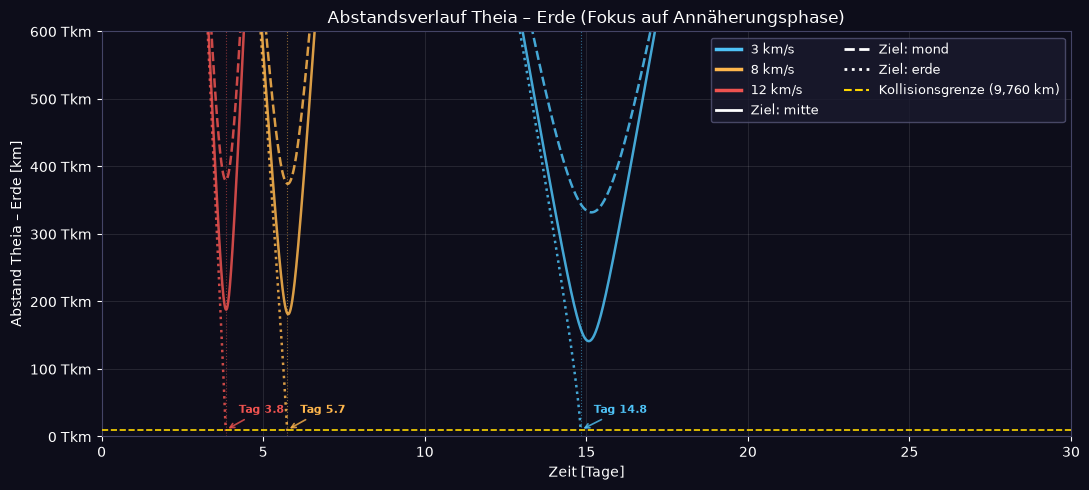
\includegraphics[keepaspectratio]{img/diagram_theia.png}}
\caption{Bild}
\end{figure}

    \subsection{Beobachtungen}\label{beobachtungen}

Die Tabelle oben fasst alle neun Konfigurationen zusammen: pro Fall, ob
(und mit welchem Körper) Theia verschmolzen ist, an welchem Tag dies
geschah, sowie den kleinsten Abstand, den Theia jeweils zur Erde und zum
Mond erreicht hat. Das Abstandsdiagramm zeigt ergänzend den zeitlichen
Verlauf des Erde-Theia-Abstands für alle neun Läufe.

\textbf{Zentrale Beobachtungen (für das Raster 3 / 8 / 12 km/s):}

\begin{itemize}
\item
  \textbf{Richtung „Erde'':} In allen drei Geschwindigkeiten kollidiert
  Theia mit der Erde. Da der Geschwindigkeitsvektor direkt auf die Erde
  zeigt und die Gravitation entlang derselben Achse wirkt, gibt es
  keinen seitlichen Ablenkungseffekt -- Theia wird nur zusätzlich
  beschleunigt und trifft unausweichlich. Die Flugzeit bis zum Einschlag
  sinkt mit steigender Geschwindigkeit deutlich (von \textasciitilde14,8
  Tagen bei 3 km/s auf \textasciitilde3,8 Tage bei 12 km/s).
\item
  \textbf{Richtung „Mond'' und „Mitte'':} Hier fliegt Theia am System
  vorbei und wird gravitativ abgelenkt (Flyby). Der minimale Erdabstand
  liegt durchweg im Bereich von \textasciitilde140.000 bis
  \textasciitilde380.000 km -- weit über der Kollisionsgrenze. Dem Mond
  kommt Theia in einzelnen Fällen aber deutlich näher (bis
  \textasciitilde50.000 km bei 8 km/s Richtung Mitte), wie die Spalte
  „Min-Abst. Mond'' in der Tabelle zeigt.
\item
  \textbf{Einfluss der Geschwindigkeit:} Eine höhere Geschwindigkeit
  verkürzt die Flugzeit und lässt der Gravitation weniger Zeit, die Bahn
  zu krümmen. Beim direkten Erd-Anflug ändert das nichts am Ergebnis
  (Treffer bleibt Treffer), beschleunigt aber den Einschlag. Bei den
  seitlichen Anflügen bleibt der Vorbeiflug erhalten.
\end{itemize}

\textbf{Antwort auf die Leitfrage}

Ja, es gibt kollisionsfreie Konfigurationen. Entscheidend ist die
Zielrichtung, nicht die Geschwindigkeit: Zielt Theia direkt auf die
Erde, kommt es bei allen drei getesteten Geschwindigkeiten zur
Kollision. Zielt sie dagegen auf den Mond oder die Mitte, fliegt sie in
allen drei Geschwindigkeiten am System vorbei. Die Geschwindigkeit
verändert nur die Flugzeit und die Bahnkrümmung, nicht aber das
grundsätzliche „Treffer-oder-Vorbeiflug''-Ergebnis.

    \begin{tcolorbox}[breakable, size=fbox, boxrule=1pt, pad at break*=1mm,colback=cellbackground, colframe=cellborder]
\prompt{In}{incolor}{21}{\boxspacing}
\begin{Verbatim}[commandchars=\\\{\}]
\PY{c+c1}{\PYZsh{} ============================================================================}
\PY{c+c1}{\PYZsh{} Repraesentativer KOLLISIONS\PYZhy{}Fall: erstes Szenario der 3x3\PYZhy{}Matrix mit Einschlag.}
\PY{c+c1}{\PYZsh{} ============================================================================}

\PY{n}{view} \PY{o}{=} \PY{l+s+s1}{\PYZsq{}}\PY{l+s+s1}{top}\PY{l+s+s1}{\PYZsq{}}
\PY{c+c1}{\PYZsh{} view = \PYZsq{}side\PYZsq{}}
\PY{c+c1}{\PYZsh{} view = \PYZsq{}standard\PYZsq{}}

\PY{n}{kollisions\PYZus{}faelle} \PY{o}{=} \PY{p}{[}\PY{n}{r} \PY{k}{for} \PY{n}{r} \PY{o+ow}{in} \PY{n}{ergebnisse} \PY{k}{if} \PY{n}{r}\PY{p}{[}\PY{l+s+s2}{\PYZdq{}}\PY{l+s+s2}{kollision\PYZus{}mit}\PY{l+s+s2}{\PYZdq{}}\PY{p}{]} \PY{o+ow}{is} \PY{o+ow}{not} \PY{k+kc}{None}\PY{p}{]}

\PY{k}{if} \PY{n}{kollisions\PYZus{}faelle}\PY{p}{:}

    \PY{n}{r} \PY{o}{=} \PY{n}{kollisions\PYZus{}faelle}\PY{p}{[}\PY{l+m+mi}{0}\PY{p}{]}
    \PY{n+nb}{print}\PY{p}{(}\PY{l+s+sa}{f}\PY{l+s+s2}{\PYZdq{}}\PY{l+s+s2}{KOLLISION: }\PY{l+s+si}{\PYZob{}}\PY{n}{r}\PY{p}{[}\PY{l+s+s1}{\PYZsq{}}\PY{l+s+s1}{speed\PYZus{}kms}\PY{l+s+s1}{\PYZsq{}}\PY{p}{]}\PY{l+s+si}{\PYZcb{}}\PY{l+s+s2}{ km/s Richtung }\PY{l+s+s2}{\PYZsq{}}\PY{l+s+si}{\PYZob{}}\PY{n}{r}\PY{p}{[}\PY{l+s+s1}{\PYZsq{}}\PY{l+s+s1}{target}\PY{l+s+s1}{\PYZsq{}}\PY{p}{]}\PY{l+s+si}{\PYZcb{}}\PY{l+s+s2}{\PYZsq{}}\PY{l+s+s2}{ \PYZhy{}\PYZgt{} Theia trifft }\PY{l+s+si}{\PYZob{}}\PY{n}{r}\PY{p}{[}\PY{l+s+s1}{\PYZsq{}}\PY{l+s+s1}{kollision\PYZus{}mit}\PY{l+s+s1}{\PYZsq{}}\PY{p}{]}\PY{l+s+si}{\PYZcb{}}\PY{l+s+s2}{\PYZdq{}}\PY{p}{)}
    \PY{n}{sel\PYZus{}sim} \PY{o}{=} \PY{n}{sims}\PY{p}{[}\PY{p}{(}\PY{n}{r}\PY{p}{[}\PY{l+s+s2}{\PYZdq{}}\PY{l+s+s2}{speed\PYZus{}kms}\PY{l+s+s2}{\PYZdq{}}\PY{p}{]}\PY{p}{,} \PY{n}{r}\PY{p}{[}\PY{l+s+s2}{\PYZdq{}}\PY{l+s+s2}{target}\PY{l+s+s2}{\PYZdq{}}\PY{p}{]}\PY{p}{)}\PY{p}{]}

    \PY{n}{anim\PYZus{}kollision} \PY{o}{=} \PY{n}{Visualizer}\PY{p}{(}\PY{n}{sel\PYZus{}sim}\PY{p}{)}\PY{o}{.}\PY{n}{animate\PYZus{}3d}\PY{p}{(}\PY{n}{view}\PY{o}{=}\PY{n}{view}\PY{p}{,} \PY{n}{performance\PYZus{}mode}\PY{o}{=}\PY{k+kc}{True}\PY{p}{,} \PY{n}{dynamic\PYZus{}scaling}\PY{o}{=}\PY{k+kc}{True}\PY{p}{)}
    \PY{n}{anim\PYZus{}kollision\PYZus{}static} \PY{o}{=} \PY{n}{Visualizer}\PY{p}{(}\PY{n}{sel\PYZus{}sim}\PY{p}{)}\PY{o}{.}\PY{n}{animate\PYZus{}3d}\PY{p}{(}\PY{n}{view}\PY{o}{=}\PY{n}{view}\PY{p}{,} \PY{n}{performance\PYZus{}mode}\PY{o}{=}\PY{k+kc}{True}\PY{p}{,} \PY{n}{dynamic\PYZus{}scaling}\PY{o}{=}\PY{k+kc}{False}\PY{p}{)}

\PY{k}{else}\PY{p}{:}
    \PY{n+nb}{print}\PY{p}{(}\PY{l+s+s2}{\PYZdq{}}\PY{l+s+s2}{In keiner der neun Konfigurationen kam es zu einer Kollision.}\PY{l+s+s2}{\PYZdq{}}\PY{p}{)}
    \PY{n}{anim\PYZus{}kollision} \PY{o}{=} \PY{k+kc}{None}
    \PY{n}{anim\PYZus{}kollision\PYZus{}static} \PY{o}{=} \PY{k+kc}{None}

\PY{n}{display}\PY{p}{(}\PY{n}{anim\PYZus{}kollision}\PY{p}{)}
\PY{n}{display}\PY{p}{(}\PY{n}{anim\PYZus{}kollision\PYZus{}static}\PY{p}{)}
\end{Verbatim}
\end{tcolorbox}

    \begin{Verbatim}[commandchars=\\\{\}]
KOLLISION: 3 km/s Richtung 'erde' -> Theia trifft Erde
    \end{Verbatim}

    
    \begin{Verbatim}[commandchars=\\\{\}]
<IPython.core.display.HTML object>
    \end{Verbatim}

    
    
    \begin{Verbatim}[commandchars=\\\{\}]
<IPython.core.display.HTML object>
    \end{Verbatim}
\begin{figure}
\centering
\pandocbounded{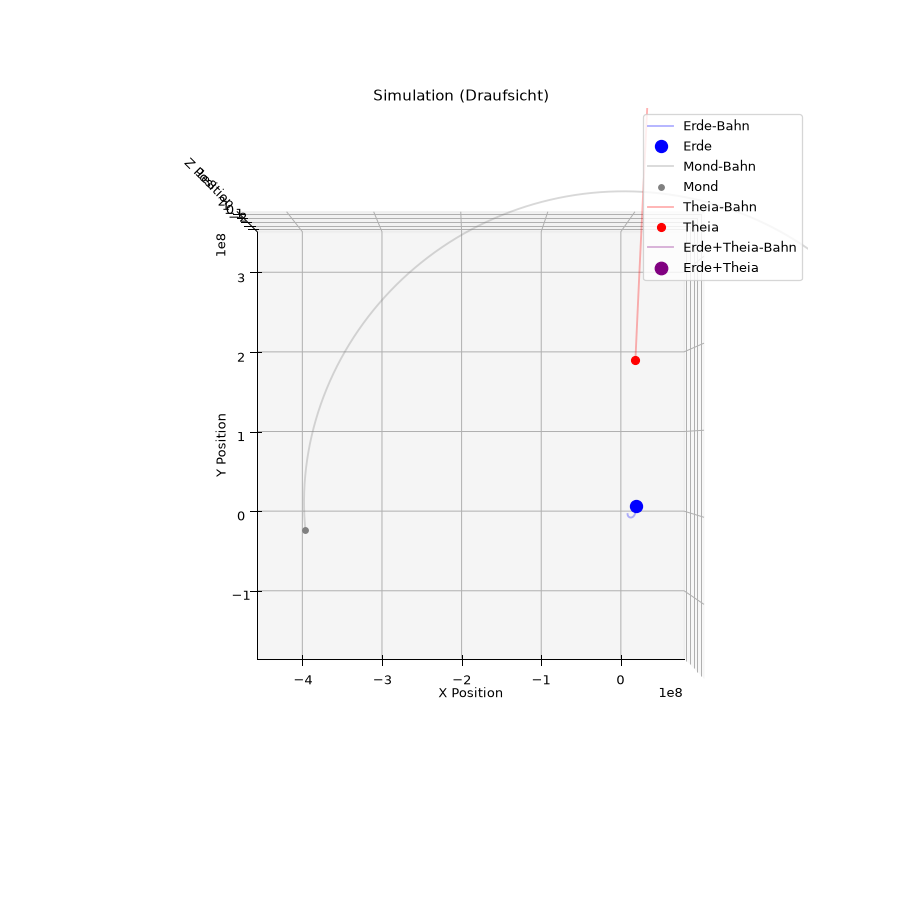
\includegraphics[keepaspectratio]{img/theia_colides_earth.png}}
\caption{Bild}
\end{figure}

    
    \begin{tcolorbox}[breakable, size=fbox, boxrule=1pt, pad at break*=1mm,colback=cellbackground, colframe=cellborder]
\prompt{In}{incolor}{22}{\boxspacing}
\begin{Verbatim}[commandchars=\\\{\}]
\PY{c+c1}{\PYZsh{} ============================================================================}
\PY{c+c1}{\PYZsh{} Repraesentativer KOLLISIONSFREIER Fall: erster Vorbeiflug der 3x3\PYZhy{}Matrix.}
\PY{c+c1}{\PYZsh{} ============================================================================}

\PY{c+c1}{\PYZsh{} view = \PYZsq{}top\PYZsq{}}
\PY{c+c1}{\PYZsh{} view = \PYZsq{}side\PYZsq{}}
\PY{n}{view} \PY{o}{=} \PY{l+s+s1}{\PYZsq{}}\PY{l+s+s1}{standard}\PY{l+s+s1}{\PYZsq{}}

\PY{n}{freie\PYZus{}faelle} \PY{o}{=} \PY{p}{[}\PY{n}{r} \PY{k}{for} \PY{n}{r} \PY{o+ow}{in} \PY{n}{ergebnisse} \PY{k}{if} \PY{n}{r}\PY{p}{[}\PY{l+s+s2}{\PYZdq{}}\PY{l+s+s2}{kollision\PYZus{}mit}\PY{l+s+s2}{\PYZdq{}}\PY{p}{]} \PY{o+ow}{is} \PY{k+kc}{None}\PY{p}{]}

\PY{k}{if} \PY{n}{freie\PYZus{}faelle}\PY{p}{:}

    \PY{n}{r} \PY{o}{=} \PY{n}{freie\PYZus{}faelle}\PY{p}{[}\PY{l+m+mi}{0}\PY{p}{]}
    \PY{n+nb}{print}\PY{p}{(}\PY{l+s+sa}{f}\PY{l+s+s2}{\PYZdq{}}\PY{l+s+s2}{KEINE Kollision: }\PY{l+s+si}{\PYZob{}}\PY{n}{r}\PY{p}{[}\PY{l+s+s1}{\PYZsq{}}\PY{l+s+s1}{speed\PYZus{}kms}\PY{l+s+s1}{\PYZsq{}}\PY{p}{]}\PY{l+s+si}{\PYZcb{}}\PY{l+s+s2}{ km/s Richtung }\PY{l+s+s2}{\PYZsq{}}\PY{l+s+si}{\PYZob{}}\PY{n}{r}\PY{p}{[}\PY{l+s+s1}{\PYZsq{}}\PY{l+s+s1}{target}\PY{l+s+s1}{\PYZsq{}}\PY{p}{]}\PY{l+s+si}{\PYZcb{}}\PY{l+s+s2}{\PYZsq{}}\PY{l+s+s2}{ }\PY{l+s+s2}{\PYZdq{}}
          \PY{l+s+sa}{f}\PY{l+s+s2}{\PYZdq{}}\PY{l+s+s2}{(min. Abstand zur Erde }\PY{l+s+si}{\PYZob{}}\PY{n}{r}\PY{p}{[}\PY{l+s+s1}{\PYZsq{}}\PY{l+s+s1}{min\PYZus{}abstand\PYZus{}erde}\PY{l+s+s1}{\PYZsq{}}\PY{p}{]}\PY{l+s+si}{:}\PY{l+s+s2}{.3e}\PY{l+s+si}{\PYZcb{}}\PY{l+s+s2}{ m, zum Mond }\PY{l+s+si}{\PYZob{}}\PY{n}{r}\PY{p}{[}\PY{l+s+s1}{\PYZsq{}}\PY{l+s+s1}{min\PYZus{}abstand\PYZus{}mond}\PY{l+s+s1}{\PYZsq{}}\PY{p}{]}\PY{l+s+si}{:}\PY{l+s+s2}{.3e}\PY{l+s+si}{\PYZcb{}}\PY{l+s+s2}{ m)}\PY{l+s+s2}{\PYZdq{}}\PY{p}{)}
    \PY{n}{sel\PYZus{}sim} \PY{o}{=} \PY{n}{sims}\PY{p}{[}\PY{p}{(}\PY{n}{r}\PY{p}{[}\PY{l+s+s2}{\PYZdq{}}\PY{l+s+s2}{speed\PYZus{}kms}\PY{l+s+s2}{\PYZdq{}}\PY{p}{]}\PY{p}{,} \PY{n}{r}\PY{p}{[}\PY{l+s+s2}{\PYZdq{}}\PY{l+s+s2}{target}\PY{l+s+s2}{\PYZdq{}}\PY{p}{]}\PY{p}{)}\PY{p}{]}

    \PY{n}{anim\PYZus{}frei} \PY{o}{=} \PY{n}{Visualizer}\PY{p}{(}\PY{n}{sel\PYZus{}sim}\PY{p}{)}\PY{o}{.}\PY{n}{animate\PYZus{}3d}\PY{p}{(}\PY{n}{view}\PY{o}{=}\PY{n}{view}\PY{p}{,} \PY{n}{performance\PYZus{}mode}\PY{o}{=}\PY{k+kc}{True}\PY{p}{,} \PY{n}{dynamic\PYZus{}scaling}\PY{o}{=}\PY{k+kc}{True}\PY{p}{)}
    \PY{n}{anim\PYZus{}frei\PYZus{}static} \PY{o}{=} \PY{n}{Visualizer}\PY{p}{(}\PY{n}{sel\PYZus{}sim}\PY{p}{)}\PY{o}{.}\PY{n}{animate\PYZus{}3d}\PY{p}{(}\PY{n}{view}\PY{o}{=}\PY{n}{view}\PY{p}{,} \PY{n}{performance\PYZus{}mode}\PY{o}{=}\PY{k+kc}{True}\PY{p}{,} \PY{n}{dynamic\PYZus{}scaling}\PY{o}{=}\PY{k+kc}{False}\PY{p}{)}

\PY{k}{else}\PY{p}{:}
    \PY{n+nb}{print}\PY{p}{(}\PY{l+s+s2}{\PYZdq{}}\PY{l+s+s2}{Jede der neun Konfigurationen führte zu einer Kollision – kein kollisionsfreier Fall vorhanden.}\PY{l+s+s2}{\PYZdq{}}\PY{p}{)}
    \PY{n}{anim\PYZus{}frei} \PY{o}{=} \PY{k+kc}{None}
    \PY{n}{anim\PYZus{}frei\PYZus{}static} \PY{o}{=} \PY{k+kc}{None}

\PY{n}{display}\PY{p}{(}\PY{n}{anim\PYZus{}frei}\PY{p}{)}
\PY{n}{display}\PY{p}{(}\PY{n}{anim\PYZus{}frei\PYZus{}static}\PY{p}{)}
\end{Verbatim}
\end{tcolorbox}

    \begin{Verbatim}[commandchars=\\\{\}]
KEINE Kollision: 3 km/s Richtung 'mitte' (min. Abstand zur Erde 1.412e+08 m, zum
Mond 3.823e+08 m)
    \end{Verbatim}

    
    \begin{Verbatim}[commandchars=\\\{\}]
<IPython.core.display.HTML object>
    \end{Verbatim}

    
    
    \begin{Verbatim}[commandchars=\\\{\}]
<IPython.core.display.HTML object>
    \end{Verbatim}

\begin{figure}
\centering
\pandocbounded{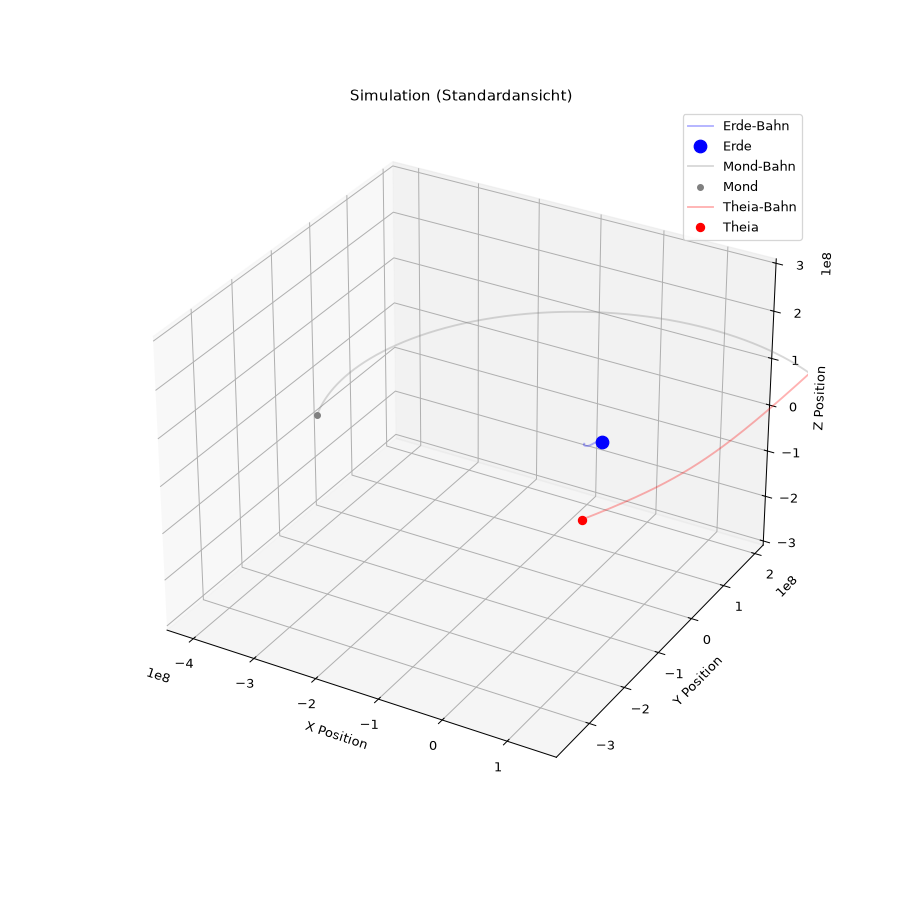
\includegraphics[keepaspectratio]{img/theia_misses_earth.png}}
\caption{Bild}
\end{figure}
    
\subsection{Bonus: Mond-Crash und Doppel-Crash}

\textbf{Wie wir diese Kombinationen gefunden haben.} Die Werte sind
nicht geraten. Um die schmalen Fenster aufzuspüren, haben wir dieselbe
Funktion \texttt{run\_theia\_scenario} in einem \textbf{feinen
Geschwindigkeits-Sweep} (Schrittweite ca. 0,05--0,1 km/s) über den
gesamten Bereich laufen lassen und für jeden Lauf das Feld
\texttt{kollision\_mit} aus dem Ergebnis-Dictionary ausgewertet. So
lässt sich genau ablesen, ab welcher Geschwindigkeit das Verhalten
umschlägt (Vorbeiflug → Mond-Treffer → Erd-Treffer). Diese systematische
Suche -- das automatisierte Durchprobieren der vielen Zwischenwerte und
das Eingrenzen der Treffer-Bereiche -- haben wir mit Unterstützung des
KI-Assistenten \textbf{Claude} durchgeführt, der den
Geschwindigkeitsbereich gezielt durchgegangen ist. Dabei zeigt sich,
\textbf{wie schmal} diese Fenster tatsächlich sind:

\begin{itemize}
\tightlist
\item
  \textbf{Mond-Crash:} Richtung \texttt{mond} trifft Theia den Mond
  praktisch nur in einem \textbf{hauchdünnen Fenster um $\approx$ 2,0 km/s} --
  bei 0,05 km/s Schrittweite trifft ausschließlich \texttt{2,00} km/s,
  während \texttt{1,95} und \texttt{2,05} km/s schon vorbeifliegen. Bei
  dieser Geschwindigkeit erreicht Theia den Mond erst nach
  \textasciitilde24 Tagen genau dann, wenn er auf seiner Bahn an der
  richtigen Stelle steht. Der entstehende Klumpen verlässt anschließend
  das System (kein Erd-Treffer).
\item
  \textbf{Doppel-Crash:} Richtung \texttt{erde} werden \textbf{beide}
  Körper nur im schmalen Band \textbf{$\approx$ 6,1--6,3 km/s} getroffen. Hier
  streift Theia auf dem Weg zur Erde zuerst den Mond (\textasciitilde6,7
  Tage) und stürzt dann in die Erde (\textasciitilde7,4 Tage). Schon ab
  \textasciitilde6,4 km/s ist Theia zu schnell, „überholt'' den Mond und
  fliegt direkt in die Erde -- ein reiner Erd-Treffer.
\end{itemize}

Als repräsentative Werte zeigen wir unten \texttt{2,0\ km/s} (Mond) und
\texttt{6,2\ km/s} (Doppel).

    \begin{tcolorbox}[breakable, size=fbox, boxrule=1pt, pad at break*=1mm,colback=cellbackground, colframe=cellborder]
\prompt{In}{incolor}{24}{\boxspacing}
\begin{Verbatim}[commandchars=\\\{\}]
\PY{c+c1}{\PYZsh{} ============================================================================}
\PY{c+c1}{\PYZsh{} BONUS MOND\PYZhy{}CRASH: Theia trifft gezielt den Mond.}
\PY{c+c1}{\PYZsh{} ============================================================================}

\PY{n}{view} \PY{o}{=} \PY{l+s+s1}{\PYZsq{}}\PY{l+s+s1}{top}\PY{l+s+s1}{\PYZsq{}}
\PY{c+c1}{\PYZsh{} view = \PYZsq{}side\PYZsq{}}
\PY{c+c1}{\PYZsh{} view = \PYZsq{}standard\PYZsq{}}

\PY{c+c1}{\PYZsh{} Eigener Lauf ausserhalb der 3x3\PYZhy{}Matrix: 2.0 km/s Richtung Mond, 50 Tage lang}
\PY{n}{sim\PYZus{}mond}\PY{p}{,} \PY{n}{res\PYZus{}mond} \PY{o}{=} \PY{n}{run\PYZus{}theia\PYZus{}scenario}\PY{p}{(}\PY{l+m+mf}{2.0}\PY{p}{,} \PY{l+s+s2}{\PYZdq{}}\PY{l+s+s2}{mond}\PY{l+s+s2}{\PYZdq{}}\PY{p}{,} \PY{n}{total\PYZus{}time}\PY{o}{=}\PY{l+m+mi}{50}\PY{p}{)}

\PY{c+c1}{\PYZsh{} Welcher Koerper wurde getroffen?}
\PY{n+nb}{print}\PY{p}{(}\PY{l+s+sa}{f}\PY{l+s+s2}{\PYZdq{}}\PY{l+s+s2}{MOND\PYZhy{}CRASH: 2.0 km/s Richtung }\PY{l+s+s2}{\PYZsq{}}\PY{l+s+s2}{mond}\PY{l+s+s2}{\PYZsq{}}\PY{l+s+s2}{ \PYZhy{}\PYZgt{} Theia trifft: }\PY{l+s+si}{\PYZob{}}\PY{n}{res\PYZus{}mond}\PY{p}{[}\PY{l+s+s1}{\PYZsq{}}\PY{l+s+s1}{kollision\PYZus{}mit}\PY{l+s+s1}{\PYZsq{}}\PY{p}{]}\PY{l+s+si}{\PYZcb{}}\PY{l+s+s2}{\PYZdq{}}\PY{p}{)}

\PY{c+c1}{\PYZsh{} Zusaetzlich den kleinsten Abstand zur Erde ausgeben.}
\PY{n+nb}{print}\PY{p}{(}\PY{l+s+sa}{f}\PY{l+s+s2}{\PYZdq{}}\PY{l+s+s2}{(Kleinster Abstand zur Erde: }\PY{l+s+si}{\PYZob{}}\PY{n}{res\PYZus{}mond}\PY{p}{[}\PY{l+s+s1}{\PYZsq{}}\PY{l+s+s1}{min\PYZus{}abstand\PYZus{}erde}\PY{l+s+s1}{\PYZsq{}}\PY{p}{]}\PY{l+s+si}{:}\PY{l+s+s2}{.3e}\PY{l+s+si}{\PYZcb{}}\PY{l+s+s2}{ m)}\PY{l+s+s2}{\PYZdq{}}\PY{p}{)}

\PY{n}{anim\PYZus{}mond\PYZus{}crash} \PY{o}{=} \PY{n}{Visualizer}\PY{p}{(}\PY{n}{sim\PYZus{}mond}\PY{p}{)}\PY{o}{.}\PY{n}{animate\PYZus{}3d}\PY{p}{(}\PY{n}{view}\PY{o}{=}\PY{n}{view}\PY{p}{,} \PY{n}{performance\PYZus{}mode}\PY{o}{=}\PY{k+kc}{True}\PY{p}{,} \PY{n}{dynamic\PYZus{}scaling}\PY{o}{=}\PY{k+kc}{True}\PY{p}{)}
\PY{n}{anim\PYZus{}mond\PYZus{}crash\PYZus{}static} \PY{o}{=} \PY{n}{Visualizer}\PY{p}{(}\PY{n}{sim\PYZus{}mond}\PY{p}{)}\PY{o}{.}\PY{n}{animate\PYZus{}3d}\PY{p}{(}\PY{n}{view}\PY{o}{=}\PY{n}{view}\PY{p}{,} \PY{n}{performance\PYZus{}mode}\PY{o}{=}\PY{k+kc}{True}\PY{p}{,} \PY{n}{dynamic\PYZus{}scaling}\PY{o}{=}\PY{k+kc}{False}\PY{p}{)}

\PY{n}{display}\PY{p}{(}\PY{n}{anim\PYZus{}mond\PYZus{}crash}\PY{p}{)}
\PY{n}{display}\PY{p}{(}\PY{n}{anim\PYZus{}mond\PYZus{}crash\PYZus{}static}\PY{p}{)}
\end{Verbatim}
\end{tcolorbox}

    \begin{Verbatim}[commandchars=\\\{\}]
Theia erfolgreich Richtung 'mond' injiziert.
MOND-CRASH: 2.0 km/s Richtung 'mond' -> Theia trifft: Mond
(Kleinster Abstand zur Erde: 2.914e+08 m)
    \end{Verbatim}

    
    \begin{Verbatim}[commandchars=\\\{\}]
<IPython.core.display.HTML object>
    \end{Verbatim}

    
    
    \begin{Verbatim}[commandchars=\\\{\}]
<IPython.core.display.HTML object>
    \end{Verbatim}
\begin{figure}
\centering
\pandocbounded{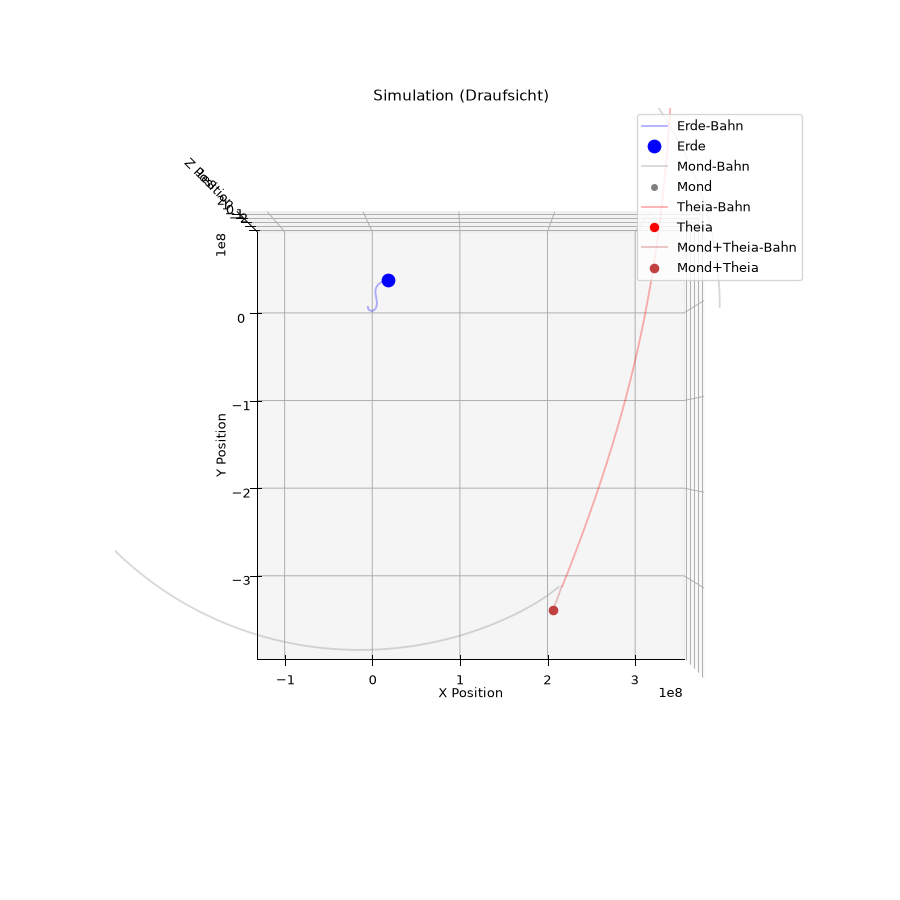
\includegraphics[keepaspectratio]{img/theia_colides_moon.png}}
\caption{Bild}
\end{figure}

    
    \begin{tcolorbox}[breakable, size=fbox, boxrule=1pt, pad at break*=1mm,colback=cellbackground, colframe=cellborder]
\prompt{In}{incolor}{23}{\boxspacing}
\begin{Verbatim}[commandchars=\\\{\}]
\PY{c+c1}{\PYZsh{} ============================================================================}
\PY{c+c1}{\PYZsh{} BONUS DOPPEL\PYZhy{}CRASH: Theia trifft in einem einzigen Anflug BEIDE Koerper.}
\PY{c+c1}{\PYZsh{} ============================================================================}

\PY{n}{view} \PY{o}{=} \PY{l+s+s1}{\PYZsq{}}\PY{l+s+s1}{top}\PY{l+s+s1}{\PYZsq{}}
\PY{c+c1}{\PYZsh{} view = \PYZsq{}side\PYZsq{}}
\PY{c+c1}{\PYZsh{} view = \PYZsq{}standard\PYZsq{}}

\PY{c+c1}{\PYZsh{} Eigener Lauf bei 6.2 km/s Richtung Erde, 20 Tage lang}
\PY{n}{sim\PYZus{}doppel}\PY{p}{,} \PY{n}{res\PYZus{}doppel} \PY{o}{=} \PY{n}{run\PYZus{}theia\PYZus{}scenario}\PY{p}{(}\PY{l+m+mf}{6.2}\PY{p}{,} \PY{l+s+s2}{\PYZdq{}}\PY{l+s+s2}{erde}\PY{l+s+s2}{\PYZdq{}}\PY{p}{,} \PY{n}{total\PYZus{}time}\PY{o}{=}\PY{l+m+mi}{20}\PY{p}{)}
\PY{n+nb}{print}\PY{p}{(}\PY{l+s+sa}{f}\PY{l+s+s2}{\PYZdq{}}\PY{l+s+s2}{DOPPEL\PYZhy{}CRASH: 6.2 km/s Richtung }\PY{l+s+s2}{\PYZsq{}}\PY{l+s+s2}{erde}\PY{l+s+s2}{\PYZsq{}}\PY{l+s+s2}{ \PYZhy{}\PYZgt{} Theia trifft: }\PY{l+s+si}{\PYZob{}}\PY{n}{res\PYZus{}doppel}\PY{p}{[}\PY{l+s+s1}{\PYZsq{}}\PY{l+s+s1}{kollision\PYZus{}mit}\PY{l+s+s1}{\PYZsq{}}\PY{p}{]}\PY{l+s+si}{\PYZcb{}}\PY{l+s+s2}{\PYZdq{}}\PY{p}{)}

\PY{n}{anim\PYZus{}doppel\PYZus{}crash} \PY{o}{=} \PY{n}{Visualizer}\PY{p}{(}\PY{n}{sim\PYZus{}doppel}\PY{p}{)}\PY{o}{.}\PY{n}{animate\PYZus{}3d}\PY{p}{(}\PY{n}{view}\PY{o}{=}\PY{n}{view}\PY{p}{,} \PY{n}{performance\PYZus{}mode}\PY{o}{=}\PY{k+kc}{True}\PY{p}{,} \PY{n}{dynamic\PYZus{}scaling}\PY{o}{=}\PY{k+kc}{True}\PY{p}{)}
\PY{n}{anim\PYZus{}doppel\PYZus{}crash\PYZus{}static} \PY{o}{=} \PY{n}{Visualizer}\PY{p}{(}\PY{n}{sim\PYZus{}doppel}\PY{p}{)}\PY{o}{.}\PY{n}{animate\PYZus{}3d}\PY{p}{(}\PY{n}{view}\PY{o}{=}\PY{n}{view}\PY{p}{,} \PY{n}{performance\PYZus{}mode}\PY{o}{=}\PY{k+kc}{True}\PY{p}{,} \PY{n}{dynamic\PYZus{}scaling}\PY{o}{=}\PY{k+kc}{False}\PY{p}{)}

\PY{n}{display}\PY{p}{(}\PY{n}{anim\PYZus{}doppel\PYZus{}crash}\PY{p}{)}
\PY{n}{display}\PY{p}{(}\PY{n}{anim\PYZus{}doppel\PYZus{}crash\PYZus{}static}\PY{p}{)}
\end{Verbatim}
\end{tcolorbox}

    \begin{Verbatim}[commandchars=\\\{\}]
Theia erfolgreich Richtung 'erde' injiziert.
DOPPEL-CRASH: 6.2 km/s Richtung 'erde' -> Theia trifft: Erde+Mond
    \end{Verbatim}

    
    \begin{Verbatim}[commandchars=\\\{\}]
<IPython.core.display.HTML object>
    \end{Verbatim}

    
    
    \begin{Verbatim}[commandchars=\\\{\}]
<IPython.core.display.HTML object>
    \end{Verbatim}
\begin{figure}
\centering
\pandocbounded{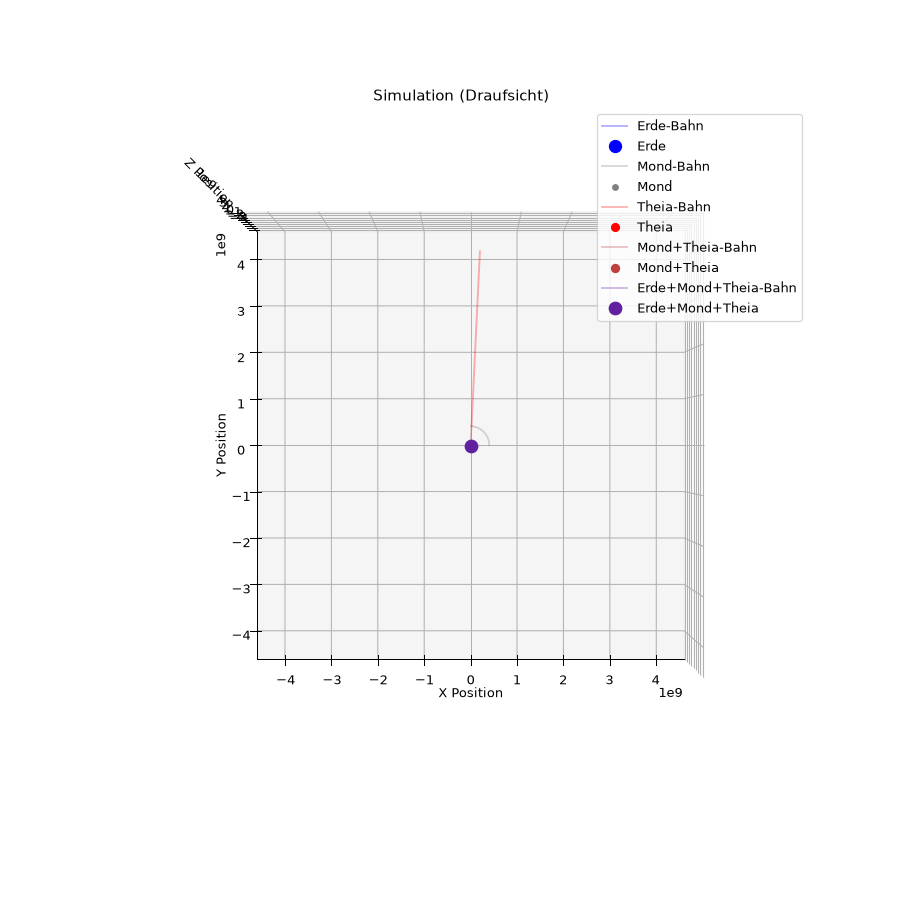
\includegraphics[keepaspectratio]{img/theia_colides_both.png}}
\caption{Bild}
\end{figure}

    \section{UnitTests}\label{unittests}

Zur Verifikation der Korrektheit des Programmentwurfs wurde eine
automatisierte Testsuite basierend auf dem Python-Framework unittest
implementiert. Diese stellt sicher, dass Modifikationen am System keine
mathematischen Regressionen verursachen.

    \begin{tcolorbox}[breakable, size=fbox, boxrule=1pt, pad at break*=1mm,colback=cellbackground, colframe=cellborder]
\prompt{In}{incolor}{ }{\boxspacing}
\begin{Verbatim}[commandchars=\\\{\}]
\PY{k+kn}{import}\PY{+w}{ }\PY{n+nn}{unittest}

\PY{k}{class}\PY{+w}{ }\PY{n+nc}{TestBody}\PY{p}{(}\PY{n}{unittest}\PY{o}{.}\PY{n}{TestCase}\PY{p}{)}\PY{p}{:}
\PY{+w}{    }\PY{l+s+sd}{\PYZdq{}\PYZdq{}\PYZdq{}}
\PY{l+s+sd}{    Unittests für den Body\PYZhy{}Datentyp}
\PY{l+s+sd}{    \PYZdq{}\PYZdq{}\PYZdq{}} 

    \PY{k}{def}\PY{+w}{ }\PY{n+nf}{setUp}\PY{p}{(}\PY{n+nb+bp}{self}\PY{p}{)}\PY{p}{:}
        \PY{c+c1}{\PYZsh{}Variablen initialisieren}
        \PY{n+nb+bp}{self}\PY{o}{.}\PY{n}{body\PYZus{}a} \PY{o}{=} \PY{n}{Body}\PY{p}{(}\PY{l+s+s2}{\PYZdq{}}\PY{l+s+s2}{Erde}\PY{l+s+s2}{\PYZdq{}}\PY{p}{,} \PY{p}{[}\PY{l+m+mi}{0}\PY{p}{,} \PY{l+m+mi}{0}\PY{p}{,} \PY{l+m+mi}{0}\PY{p}{]}\PY{p}{,} \PY{p}{[}\PY{l+m+mi}{0}\PY{p}{,} \PY{l+m+mi}{0}\PY{p}{,} \PY{l+m+mi}{0}\PY{p}{]}\PY{p}{,} \PY{n}{radius}\PY{o}{=}\PY{l+m+mf}{100.0}\PY{p}{,} \PY{n}{mass}\PY{o}{=}\PY{l+m+mf}{50.0}\PY{p}{,} \PY{n}{color}\PY{o}{=}\PY{l+s+s2}{\PYZdq{}}\PY{l+s+s2}{blue}\PY{l+s+s2}{\PYZdq{}}\PY{p}{)}
        \PY{n+nb+bp}{self}\PY{o}{.}\PY{n}{body\PYZus{}b} \PY{o}{=} \PY{n}{Body}\PY{p}{(}\PY{l+s+s2}{\PYZdq{}}\PY{l+s+s2}{Mond}\PY{l+s+s2}{\PYZdq{}}\PY{p}{,} \PY{p}{[}\PY{l+m+mi}{300}\PY{p}{,} \PY{l+m+mi}{0}\PY{p}{,} \PY{l+m+mi}{0}\PY{p}{]}\PY{p}{,} \PY{p}{[}\PY{l+m+mi}{0}\PY{p}{,} \PY{l+m+mi}{20}\PY{p}{,} \PY{l+m+mi}{0}\PY{p}{]}\PY{p}{,} \PY{n}{radius}\PY{o}{=}\PY{l+m+mf}{20.0}\PY{p}{,} \PY{n}{mass}\PY{o}{=}\PY{l+m+mf}{5.0}\PY{p}{,} \PY{n}{color}\PY{o}{=}\PY{l+s+s2}{\PYZdq{}}\PY{l+s+s2}{gray}\PY{l+s+s2}{\PYZdq{}}\PY{p}{)}
        
    \PY{k}{def}\PY{+w}{ }\PY{n+nf}{test\PYZus{}01\PYZus{}init}\PY{p}{(}\PY{n+nb+bp}{self}\PY{p}{)}\PY{p}{:}
        \PY{c+c1}{\PYZsh{}Testen, ob init\PYZhy{}Methode fehlerfrei funktioniert}
        \PY{n+nb+bp}{self}\PY{o}{.}\PY{n}{assertEqual}\PY{p}{(}\PY{n+nb+bp}{self}\PY{o}{.}\PY{n}{body\PYZus{}a}\PY{o}{.}\PY{n}{name}\PY{p}{,} \PY{l+s+s2}{\PYZdq{}}\PY{l+s+s2}{Erde}\PY{l+s+s2}{\PYZdq{}}\PY{p}{)}
        \PY{n}{np}\PY{o}{.}\PY{n}{testing}\PY{o}{.}\PY{n}{assert\PYZus{}array\PYZus{}equal}\PY{p}{(}\PY{n+nb+bp}{self}\PY{o}{.}\PY{n}{body\PYZus{}b}\PY{o}{.}\PY{n}{position}\PY{p}{,} \PY{n}{np}\PY{o}{.}\PY{n}{array}\PY{p}{(}\PY{p}{[}\PY{l+m+mi}{300}\PY{p}{,} \PY{l+m+mi}{0}\PY{p}{,} \PY{l+m+mi}{0}\PY{p}{]}\PY{p}{,} \PY{n}{dtype}\PY{o}{=}\PY{n+nb}{float}\PY{p}{)}\PY{p}{)}
        \PY{n+nb+bp}{self}\PY{o}{.}\PY{n}{assertIsInstance}\PY{p}{(}\PY{n+nb+bp}{self}\PY{o}{.}\PY{n}{body\PYZus{}b}\PY{o}{.}\PY{n}{velocity}\PY{p}{,} \PY{n}{np}\PY{o}{.}\PY{n}{ndarray}\PY{p}{)}
        
    \PY{k}{def}\PY{+w}{ }\PY{n+nf}{test\PYZus{}02\PYZus{}distance}\PY{p}{(}\PY{n+nb+bp}{self}\PY{p}{)}\PY{p}{:}
        \PY{c+c1}{\PYZsh{} Testen, ob Distanz\PYZhy{}Funktion fehlerfrei funktioniert}
        \PY{n}{distance} \PY{o}{=} \PY{n+nb+bp}{self}\PY{o}{.}\PY{n}{body\PYZus{}a}\PY{o}{.}\PY{n}{get\PYZus{}distance\PYZus{}to\PYZus{}body}\PY{p}{(}\PY{n+nb+bp}{self}\PY{o}{.}\PY{n}{body\PYZus{}b}\PY{p}{)}
        \PY{c+c1}{\PYZsh{}Selbst errechneter Abstand = 300.0}
        \PY{n+nb+bp}{self}\PY{o}{.}\PY{n}{assertEqual}\PY{p}{(}\PY{n}{distance}\PY{p}{,} \PY{l+m+mf}{300.0}\PY{p}{)}
        \PY{n+nb+bp}{self}\PY{o}{.}\PY{n}{assertIsInstance}\PY{p}{(}\PY{n}{distance}\PY{p}{,} \PY{n+nb}{float}\PY{p}{)}
        
    \PY{k}{def}\PY{+w}{ }\PY{n+nf}{test\PYZus{}03\PYZus{}changePosition}\PY{p}{(}\PY{n+nb+bp}{self}\PY{p}{)}\PY{p}{:}
        \PY{c+c1}{\PYZsh{} Testen, ob update\PYZus{}position Funktion fehlerfrei funktioniert}
        \PY{n+nb+bp}{self}\PY{o}{.}\PY{n}{body\PYZus{}b}\PY{o}{.}\PY{n}{update\PYZus{}position}\PY{p}{(}\PY{l+m+mf}{10.0}\PY{p}{)}
        \PY{c+c1}{\PYZsh{}Abgleichen mit selbst errechnetem Ergebnis}
        \PY{n}{np}\PY{o}{.}\PY{n}{testing}\PY{o}{.}\PY{n}{assert\PYZus{}array\PYZus{}equal}\PY{p}{(}\PY{n+nb+bp}{self}\PY{o}{.}\PY{n}{body\PYZus{}b}\PY{o}{.}\PY{n}{position}\PY{p}{,} \PY{n}{np}\PY{o}{.}\PY{n}{array}\PY{p}{(}\PY{p}{[}\PY{l+m+mi}{300}\PY{p}{,} \PY{l+m+mi}{200}\PY{p}{,} \PY{l+m+mi}{0}\PY{p}{]}\PY{p}{,} \PY{n}{dtype}\PY{o}{=}\PY{n+nb}{float}\PY{p}{)}\PY{p}{)}
        
    \PY{k}{def}\PY{+w}{ }\PY{n+nf}{test\PYZus{}04\PYZus{}changeVelocricity}\PY{p}{(}\PY{n+nb+bp}{self}\PY{p}{)}\PY{p}{:}
        \PY{c+c1}{\PYZsh{} Testen, ob update\PYZus{}velocity Funktion fehlerfrei funktioniert}
        \PY{n}{acceleration} \PY{o}{=} \PY{n}{np}\PY{o}{.}\PY{n}{array}\PY{p}{(}\PY{p}{[}\PY{l+m+mi}{5}\PY{p}{,}\PY{l+m+mi}{0}\PY{p}{,}\PY{l+m+mi}{0}\PY{p}{]}\PY{p}{,} \PY{n}{dtype}\PY{o}{=}\PY{n+nb}{float}\PY{p}{)}
        \PY{n+nb+bp}{self}\PY{o}{.}\PY{n}{body\PYZus{}b}\PY{o}{.}\PY{n}{update\PYZus{}velocity}\PY{p}{(}\PY{n}{acceleration}\PY{p}{,}\PY{l+m+mf}{10.0}\PY{p}{)}
        \PY{c+c1}{\PYZsh{}Selbst errechnetes Ergebnis}
        \PY{n}{expectedVelocricity} \PY{o}{=} \PY{n}{np}\PY{o}{.}\PY{n}{array}\PY{p}{(}\PY{p}{[}\PY{l+m+mi}{50}\PY{p}{,}\PY{l+m+mi}{20}\PY{p}{,}\PY{l+m+mi}{0}\PY{p}{]}\PY{p}{,} \PY{n}{dtype}\PY{o}{=}\PY{n+nb}{float}\PY{p}{)}
        \PY{n}{np}\PY{o}{.}\PY{n}{testing}\PY{o}{.}\PY{n}{assert\PYZus{}array\PYZus{}equal}\PY{p}{(}\PY{n+nb+bp}{self}\PY{o}{.}\PY{n}{body\PYZus{}b}\PY{o}{.}\PY{n}{velocity}\PY{p}{,} \PY{n}{expectedVelocricity}\PY{p}{)}
        
    \PY{k}{def}\PY{+w}{ }\PY{n+nf}{test\PYZus{}05\PYZus{}getMomentum}\PY{p}{(}\PY{n+nb+bp}{self}\PY{p}{)}\PY{p}{:}
        \PY{c+c1}{\PYZsh{} Testen, ob get\PYZus{}momentum Funktion fehlerfrei Funktioniert}
        \PY{c+c1}{\PYZsh{}Selbst errechnetes Ergebnis}
        \PY{n}{expectedMomentum} \PY{o}{=} \PY{n}{np}\PY{o}{.}\PY{n}{array}\PY{p}{(}\PY{p}{[}\PY{l+m+mi}{0}\PY{p}{,}\PY{l+m+mi}{100}\PY{p}{,}\PY{l+m+mi}{0}\PY{p}{]}\PY{p}{,} \PY{n}{dtype}\PY{o}{=}\PY{n+nb}{float}\PY{p}{)}
        \PY{n}{np}\PY{o}{.}\PY{n}{testing}\PY{o}{.}\PY{n}{assert\PYZus{}array\PYZus{}equal}\PY{p}{(}\PY{n}{expectedMomentum}\PY{p}{,} \PY{n+nb+bp}{self}\PY{o}{.}\PY{n}{body\PYZus{}b}\PY{o}{.}\PY{n}{get\PYZus{}momentum}\PY{p}{(}\PY{p}{)}\PY{p}{)}     
\end{Verbatim}
\end{tcolorbox}

    \begin{tcolorbox}[breakable, size=fbox, boxrule=1pt, pad at break*=1mm,colback=cellbackground, colframe=cellborder]
\prompt{In}{incolor}{ }{\boxspacing}
\begin{Verbatim}[commandchars=\\\{\}]
\PY{k}{class}\PY{+w}{ }\PY{n+nc}{TestSimulation}\PY{p}{(}\PY{n}{unittest}\PY{o}{.}\PY{n}{TestCase}\PY{p}{)}\PY{p}{:}
\PY{+w}{    }\PY{l+s+sd}{\PYZdq{}\PYZdq{}\PYZdq{}}
\PY{l+s+sd}{    Unittests für die Simulation}
\PY{l+s+sd}{    \PYZdq{}\PYZdq{}\PYZdq{}} 
    \PY{k}{def}\PY{+w}{ }\PY{n+nf}{setUp}\PY{p}{(}\PY{n+nb+bp}{self}\PY{p}{)}\PY{p}{:}
        \PY{n+nb+bp}{self}\PY{o}{.}\PY{n}{body\PYZus{}1} \PY{o}{=} \PY{n}{Body}\PY{p}{(}\PY{l+s+s2}{\PYZdq{}}\PY{l+s+s2}{Körper1}\PY{l+s+s2}{\PYZdq{}}\PY{p}{,} \PY{p}{[}\PY{l+m+mi}{0}\PY{p}{,} \PY{l+m+mi}{0}\PY{p}{,} \PY{l+m+mi}{0}\PY{p}{]}\PY{p}{,} \PY{p}{[}\PY{l+m+mi}{0}\PY{p}{,} \PY{l+m+mi}{0}\PY{p}{,} \PY{l+m+mi}{0}\PY{p}{]}\PY{p}{,} \PY{n}{radius}\PY{o}{=}\PY{l+m+mf}{10.0}\PY{p}{,} \PY{n}{mass}\PY{o}{=}\PY{l+m+mi}{100}\PY{p}{,} \PY{n}{color}\PY{o}{=}\PY{l+s+s2}{\PYZdq{}}\PY{l+s+s2}{red}\PY{l+s+s2}{\PYZdq{}}\PY{p}{)}
        \PY{n+nb+bp}{self}\PY{o}{.}\PY{n}{body\PYZus{}2} \PY{o}{=} \PY{n}{Body}\PY{p}{(}\PY{l+s+s2}{\PYZdq{}}\PY{l+s+s2}{Körper2}\PY{l+s+s2}{\PYZdq{}}\PY{p}{,} \PY{p}{[}\PY{l+m+mi}{100}\PY{p}{,} \PY{l+m+mi}{0}\PY{p}{,} \PY{l+m+mi}{0}\PY{p}{]}\PY{p}{,} \PY{p}{[}\PY{l+m+mi}{0}\PY{p}{,} \PY{l+m+mi}{0}\PY{p}{,} \PY{l+m+mi}{0}\PY{p}{]}\PY{p}{,} \PY{n}{radius}\PY{o}{=}\PY{l+m+mf}{5.0}\PY{p}{,} \PY{n}{mass}\PY{o}{=}\PY{l+m+mf}{10.0}\PY{p}{,} \PY{n}{color}\PY{o}{=}\PY{l+s+s2}{\PYZdq{}}\PY{l+s+s2}{green}\PY{l+s+s2}{\PYZdq{}}\PY{p}{)}
        
        \PY{n+nb+bp}{self}\PY{o}{.}\PY{n}{simulation} \PY{o}{=} \PY{n}{Simulation}\PY{p}{(}\PY{l+m+mf}{10.0}\PY{p}{)}
        
    \PY{k}{def}\PY{+w}{ }\PY{n+nf}{test\PYZus{}01\PYZus{}addAndRemoveBody}\PY{p}{(}\PY{n+nb+bp}{self}\PY{p}{)}\PY{p}{:}
        \PY{c+c1}{\PYZsh{}Testen, ob ein Körper erfolgreich entfernt bzw. hinzugefügt wird}
        \PY{n+nb+bp}{self}\PY{o}{.}\PY{n}{simulation}\PY{o}{.}\PY{n}{add\PYZus{}body}\PY{p}{(}\PY{n+nb+bp}{self}\PY{o}{.}\PY{n}{body\PYZus{}1}\PY{p}{)}
        \PY{n+nb+bp}{self}\PY{o}{.}\PY{n}{assertEqual}\PY{p}{(}\PY{n+nb}{len}\PY{p}{(}\PY{n+nb+bp}{self}\PY{o}{.}\PY{n}{simulation}\PY{o}{.}\PY{n}{bodies}\PY{p}{)}\PY{p}{,} \PY{l+m+mi}{1}\PY{p}{)}
        
        \PY{n+nb+bp}{self}\PY{o}{.}\PY{n}{simulation}\PY{o}{.}\PY{n}{remove\PYZus{}body}\PY{p}{(}\PY{n+nb+bp}{self}\PY{o}{.}\PY{n}{body\PYZus{}1}\PY{p}{)}
        \PY{n+nb+bp}{self}\PY{o}{.}\PY{n}{assertEqual}\PY{p}{(}\PY{n+nb}{len}\PY{p}{(}\PY{n+nb+bp}{self}\PY{o}{.}\PY{n}{simulation}\PY{o}{.}\PY{n}{bodies}\PY{p}{)}\PY{p}{,} \PY{l+m+mi}{0}\PY{p}{)}
        
    \PY{k}{def}\PY{+w}{ }\PY{n+nf}{test\PYZus{}02\PYZus{}calculate\PYZus{}gravity}\PY{p}{(}\PY{n+nb+bp}{self}\PY{p}{)}\PY{p}{:}
        \PY{c+c1}{\PYZsh{}Testen, ob die Anziehungskräfte auch richtig berechnet werden, wenn die Körper sich am selben Punkt befinden}
        \PY{n+nb+bp}{self}\PY{o}{.}\PY{n}{simulation}\PY{o}{.}\PY{n}{add\PYZus{}body}\PY{p}{(}\PY{n+nb+bp}{self}\PY{o}{.}\PY{n}{body\PYZus{}1}\PY{p}{)}
        \PY{n}{body\PYZus{}3} \PY{o}{=} \PY{n}{Body}\PY{p}{(}\PY{l+s+s2}{\PYZdq{}}\PY{l+s+s2}{Körper12}\PY{l+s+s2}{\PYZdq{}}\PY{p}{,} \PY{p}{[}\PY{l+m+mi}{0}\PY{p}{,} \PY{l+m+mi}{0}\PY{p}{,} \PY{l+m+mi}{0}\PY{p}{]}\PY{p}{,} \PY{p}{[}\PY{l+m+mi}{0}\PY{p}{,} \PY{l+m+mi}{0}\PY{p}{,} \PY{l+m+mi}{0}\PY{p}{]}\PY{p}{,} \PY{n}{radius}\PY{o}{=}\PY{l+m+mf}{10.0}\PY{p}{,} \PY{n}{mass}\PY{o}{=}\PY{l+m+mi}{100}\PY{p}{,} \PY{n}{color}\PY{o}{=}\PY{l+s+s2}{\PYZdq{}}\PY{l+s+s2}{red}\PY{l+s+s2}{\PYZdq{}}\PY{p}{)}
        \PY{n+nb+bp}{self}\PY{o}{.}\PY{n}{simulation}\PY{o}{.}\PY{n}{add\PYZus{}body}\PY{p}{(}\PY{n}{body\PYZus{}3}\PY{p}{)}
        
        \PY{n}{forces} \PY{o}{=} \PY{n+nb+bp}{self}\PY{o}{.}\PY{n}{simulation}\PY{o}{.}\PY{n}{calculate\PYZus{}gravity}\PY{p}{(}\PY{p}{)}
        
        \PY{c+c1}{\PYZsh{}wenn es der gleiche Ort ist, darf es keine Anziehungskraft geben}
        \PY{n}{expectedForce} \PY{o}{=} \PY{n}{np}\PY{o}{.}\PY{n}{array}\PY{p}{(}\PY{p}{[} \PY{l+m+mf}{0.0}\PY{p}{,}  \PY{l+m+mf}{0.0}\PY{p}{,}  \PY{l+m+mf}{0.0}\PY{p}{]}\PY{p}{,} \PY{n}{dtype}\PY{o}{=}\PY{n+nb}{float}\PY{p}{)}
        
        \PY{n}{np}\PY{o}{.}\PY{n}{testing}\PY{o}{.}\PY{n}{assert\PYZus{}array\PYZus{}almost\PYZus{}equal}\PY{p}{(}\PY{n}{forces}\PY{p}{[}\PY{n+nb+bp}{self}\PY{o}{.}\PY{n}{body\PYZus{}1}\PY{o}{.}\PY{n}{name}\PY{p}{]}\PY{p}{,} \PY{n}{expectedForce}\PY{p}{,} \PY{n}{decimal}\PY{o}{=}\PY{l+m+mi}{6}\PY{p}{)}
        \PY{n}{np}\PY{o}{.}\PY{n}{testing}\PY{o}{.}\PY{n}{assert\PYZus{}array\PYZus{}almost\PYZus{}equal}\PY{p}{(}\PY{n}{forces}\PY{p}{[}\PY{n}{body\PYZus{}3}\PY{o}{.}\PY{n}{name}\PY{p}{]}\PY{p}{,} \PY{n}{expectedForce}\PY{p}{,} \PY{n}{decimal}\PY{o}{=}\PY{l+m+mi}{6}\PY{p}{)}
        
    \PY{k}{def}\PY{+w}{ }\PY{n+nf}{test\PYZus{}03\PYZus{}checkCollisions\PYZus{}true}\PY{p}{(}\PY{n+nb+bp}{self}\PY{p}{)}\PY{p}{:}
        \PY{c+c1}{\PYZsh{}Testen, ob die Funktion Kollisionen erkennt und richtig verarbeitet}
        \PY{n+nb+bp}{self}\PY{o}{.}\PY{n}{simulation}\PY{o}{.}\PY{n}{add\PYZus{}body}\PY{p}{(}\PY{n+nb+bp}{self}\PY{o}{.}\PY{n}{body\PYZus{}1}\PY{p}{)}
        \PY{n+nb+bp}{self}\PY{o}{.}\PY{n}{simulation}\PY{o}{.}\PY{n}{add\PYZus{}body}\PY{p}{(}\PY{n+nb+bp}{self}\PY{o}{.}\PY{n}{body\PYZus{}2}\PY{p}{)}
        
        \PY{c+c1}{\PYZsh{} Position so anpassen, dass die Körper kollidieren}
        \PY{n+nb+bp}{self}\PY{o}{.}\PY{n}{body\PYZus{}2}\PY{o}{.}\PY{n}{position} \PY{o}{=} \PY{n}{np}\PY{o}{.}\PY{n}{array}\PY{p}{(}\PY{p}{[}\PY{l+m+mi}{12}\PY{p}{,}\PY{l+m+mi}{0}\PY{p}{,}\PY{l+m+mi}{0}\PY{p}{]}\PY{p}{,} \PY{n}{dtype}\PY{o}{=}\PY{n+nb}{float}\PY{p}{)}
        
        \PY{n}{collision} \PY{o}{=} \PY{n+nb+bp}{self}\PY{o}{.}\PY{n}{simulation}\PY{o}{.}\PY{n}{check\PYZus{}collisions}\PY{p}{(}\PY{p}{)}
        \PY{n+nb+bp}{self}\PY{o}{.}\PY{n}{assertTrue}\PY{p}{(}\PY{n}{collision}\PY{p}{)}
        \PY{n+nb+bp}{self}\PY{o}{.}\PY{n}{assertEqual}\PY{p}{(}\PY{n+nb}{len}\PY{p}{(}\PY{n+nb+bp}{self}\PY{o}{.}\PY{n}{simulation}\PY{o}{.}\PY{n}{bodies}\PY{p}{)}\PY{p}{,} \PY{l+m+mi}{1}\PY{p}{)}
    
    \PY{k}{def}\PY{+w}{ }\PY{n+nf}{test\PYZus{}04\PYZus{}checkCollisions\PYZus{}false}\PY{p}{(}\PY{n+nb+bp}{self}\PY{p}{)}\PY{p}{:}
        \PY{c+c1}{\PYZsh{}Testen, ob die Funktion nicht kollidierende Körper erkennt und richtig verarbeitet}
        \PY{n+nb+bp}{self}\PY{o}{.}\PY{n}{simulation}\PY{o}{.}\PY{n}{add\PYZus{}body}\PY{p}{(}\PY{n+nb+bp}{self}\PY{o}{.}\PY{n}{body\PYZus{}1}\PY{p}{)}
        \PY{n+nb+bp}{self}\PY{o}{.}\PY{n}{simulation}\PY{o}{.}\PY{n}{add\PYZus{}body}\PY{p}{(}\PY{n+nb+bp}{self}\PY{o}{.}\PY{n}{body\PYZus{}2}\PY{p}{)}
        
        \PY{c+c1}{\PYZsh{}Position so anpassen, dass die Körper nicht kollidieren}
        \PY{n+nb+bp}{self}\PY{o}{.}\PY{n}{body\PYZus{}2}\PY{o}{.}\PY{n}{position} \PY{o}{=} \PY{n}{np}\PY{o}{.}\PY{n}{array}\PY{p}{(}\PY{p}{[}\PY{l+m+mi}{200}\PY{p}{,}\PY{l+m+mi}{0}\PY{p}{,}\PY{l+m+mi}{0}\PY{p}{]}\PY{p}{,} \PY{n}{dtype}\PY{o}{=}\PY{n+nb}{float}\PY{p}{)}
        
        \PY{n}{collision} \PY{o}{=} \PY{n+nb+bp}{self}\PY{o}{.}\PY{n}{simulation}\PY{o}{.}\PY{n}{check\PYZus{}collisions}\PY{p}{(}\PY{p}{)}
        \PY{n+nb+bp}{self}\PY{o}{.}\PY{n}{assertFalse}\PY{p}{(}\PY{n}{collision}\PY{p}{)}
        \PY{n+nb+bp}{self}\PY{o}{.}\PY{n}{assertEqual}\PY{p}{(}\PY{n+nb}{len}\PY{p}{(}\PY{n+nb+bp}{self}\PY{o}{.}\PY{n}{simulation}\PY{o}{.}\PY{n}{bodies}\PY{p}{)}\PY{p}{,} \PY{l+m+mi}{2}\PY{p}{)}
        
    \PY{k}{def}\PY{+w}{ }\PY{n+nf}{test\PYZus{}05\PYZus{}blendColors}\PY{p}{(}\PY{n+nb+bp}{self}\PY{p}{)}\PY{p}{:}
        \PY{c+c1}{\PYZsh{}Testen, ob die Farben richtig gemischt werden}
        \PY{n}{color} \PY{o}{=} \PY{n+nb+bp}{self}\PY{o}{.}\PY{n}{simulation}\PY{o}{.}\PY{n}{\PYZus{}blend\PYZus{}colors}\PY{p}{(}\PY{l+s+s1}{\PYZsq{}}\PY{l+s+s1}{blue}\PY{l+s+s1}{\PYZsq{}}\PY{p}{,} \PY{l+s+s1}{\PYZsq{}}\PY{l+s+s1}{red}\PY{l+s+s1}{\PYZsq{}}\PY{p}{)}
        \PY{c+c1}{\PYZsh{}selbst errechnetes Ergebnis}
        \PY{n}{violett} \PY{o}{=} \PY{p}{(}\PY{l+m+mf}{0.5}\PY{p}{,} \PY{l+m+mf}{0.0}\PY{p}{,} \PY{l+m+mf}{0.5}\PY{p}{)}
        \PY{n+nb+bp}{self}\PY{o}{.}\PY{n}{assertEqual}\PY{p}{(}\PY{n}{color}\PY{p}{,}\PY{n}{violett}\PY{p}{)}
        
    \PY{k}{def}\PY{+w}{ }\PY{n+nf}{test\PYZus{}06\PYZus{}MergeBodies}\PY{p}{(}\PY{n+nb+bp}{self}\PY{p}{)}\PY{p}{:}
        \PY{c+c1}{\PYZsh{}Testen, ob die Masse und der Radius des verschmolzenen Körpers richtig ausgerechnet und eingetragen werden}
        \PY{n+nb+bp}{self}\PY{o}{.}\PY{n}{simulation}\PY{o}{.}\PY{n}{add\PYZus{}body}\PY{p}{(}\PY{n+nb+bp}{self}\PY{o}{.}\PY{n}{body\PYZus{}1}\PY{p}{)}
        \PY{n+nb+bp}{self}\PY{o}{.}\PY{n}{simulation}\PY{o}{.}\PY{n}{add\PYZus{}body}\PY{p}{(}\PY{n+nb+bp}{self}\PY{o}{.}\PY{n}{body\PYZus{}2}\PY{p}{)}
        
        \PY{n+nb+bp}{self}\PY{o}{.}\PY{n}{body\PYZus{}2}\PY{o}{.}\PY{n}{position} \PY{o}{=} \PY{n}{np}\PY{o}{.}\PY{n}{array}\PY{p}{(}\PY{p}{[}\PY{l+m+mi}{12}\PY{p}{,}\PY{l+m+mi}{0}\PY{p}{,}\PY{l+m+mi}{0}\PY{p}{]}\PY{p}{,} \PY{n}{dtype}\PY{o}{=}\PY{n+nb}{float}\PY{p}{)}
        
        \PY{n+nb+bp}{self}\PY{o}{.}\PY{n}{simulation}\PY{o}{.}\PY{n}{merge\PYZus{}bodies}\PY{p}{(}\PY{n+nb+bp}{self}\PY{o}{.}\PY{n}{body\PYZus{}1}\PY{p}{,} \PY{n+nb+bp}{self}\PY{o}{.}\PY{n}{body\PYZus{}2}\PY{p}{)}
        
        \PY{c+c1}{\PYZsh{}weil mass1 + mass2 =110}
        \PY{n+nb+bp}{self}\PY{o}{.}\PY{n}{assertEqual}\PY{p}{(}\PY{n+nb+bp}{self}\PY{o}{.}\PY{n}{simulation}\PY{o}{.}\PY{n}{bodies}\PY{p}{[}\PY{l+m+mi}{0}\PY{p}{]}\PY{o}{.}\PY{n}{mass}\PY{p}{,} \PY{l+m+mi}{110}\PY{p}{)}
        
        \PY{n}{expected\PYZus{}radius} \PY{o}{=} \PY{p}{(}\PY{l+m+mf}{10.0}\PY{o}{*}\PY{o}{*}\PY{l+m+mi}{3} \PY{o}{+} \PY{l+m+mf}{5.0}\PY{o}{*}\PY{o}{*}\PY{l+m+mi}{3}\PY{p}{)}\PY{o}{*}\PY{o}{*}\PY{p}{(}\PY{l+m+mi}{1}\PY{o}{/}\PY{l+m+mi}{3}\PY{p}{)}
        \PY{n+nb+bp}{self}\PY{o}{.}\PY{n}{assertAlmostEqual}\PY{p}{(}\PY{n+nb+bp}{self}\PY{o}{.}\PY{n}{simulation}\PY{o}{.}\PY{n}{bodies}\PY{p}{[}\PY{l+m+mi}{0}\PY{p}{]}\PY{o}{.}\PY{n}{radius}\PY{p}{,} \PY{n}{expected\PYZus{}radius}\PY{p}{)} 
        
    \PY{k}{def}\PY{+w}{ }\PY{n+nf}{test\PYZus{}07\PYZus{}step}\PY{p}{(}\PY{n+nb+bp}{self}\PY{p}{)}\PY{p}{:}
        \PY{c+c1}{\PYZsh{} Testen, ob die step\PYZhy{}Funktion die Historie richtig aufzeichnet}
        \PY{n+nb+bp}{self}\PY{o}{.}\PY{n}{simulation}\PY{o}{.}\PY{n}{add\PYZus{}body}\PY{p}{(}\PY{n+nb+bp}{self}\PY{o}{.}\PY{n}{body\PYZus{}1}\PY{p}{)}
        
        \PY{n+nb+bp}{self}\PY{o}{.}\PY{n}{assertEqual}\PY{p}{(}\PY{n+nb+bp}{self}\PY{o}{.}\PY{n}{simulation}\PY{o}{.}\PY{n}{recorded\PYZus{}steps}\PY{p}{,} \PY{l+m+mi}{0}\PY{p}{)}   
        \PY{n+nb+bp}{self}\PY{o}{.}\PY{n}{assertEqual}\PY{p}{(}\PY{n+nb}{len}\PY{p}{(}\PY{n+nb+bp}{self}\PY{o}{.}\PY{n}{simulation}\PY{o}{.}\PY{n}{history}\PY{p}{[}\PY{l+s+s2}{\PYZdq{}}\PY{l+s+s2}{Körper1}\PY{l+s+s2}{\PYZdq{}}\PY{p}{]}\PY{p}{)}\PY{p}{,} \PY{l+m+mi}{0}\PY{p}{)} 
        
        \PY{n+nb+bp}{self}\PY{o}{.}\PY{n}{simulation}\PY{o}{.}\PY{n}{step}\PY{p}{(}\PY{p}{)}
        
        \PY{n+nb+bp}{self}\PY{o}{.}\PY{n}{assertEqual}\PY{p}{(}\PY{n+nb+bp}{self}\PY{o}{.}\PY{n}{simulation}\PY{o}{.}\PY{n}{recorded\PYZus{}steps}\PY{p}{,} \PY{l+m+mi}{1}\PY{p}{)}   
        \PY{n+nb+bp}{self}\PY{o}{.}\PY{n}{assertEqual}\PY{p}{(}\PY{n+nb}{len}\PY{p}{(}\PY{n+nb+bp}{self}\PY{o}{.}\PY{n}{simulation}\PY{o}{.}\PY{n}{history}\PY{p}{[}\PY{l+s+s2}{\PYZdq{}}\PY{l+s+s2}{Körper1}\PY{l+s+s2}{\PYZdq{}}\PY{p}{]}\PY{p}{)}\PY{p}{,} \PY{l+m+mi}{1}\PY{p}{)}  
        
    \PY{k}{def}\PY{+w}{ }\PY{n+nf}{test\PYZus{}08\PYZus{}run}\PY{p}{(}\PY{n+nb+bp}{self}\PY{p}{)}\PY{p}{:}
        \PY{c+c1}{\PYZsh{}Testen, ob die richtige Anzahl an steps mit Ausführung der run\PYZhy{}Funktion ausgeführt werden}
        \PY{c+c1}{\PYZsh{} und richtig aufgezeichnet werden}
        \PY{n+nb+bp}{self}\PY{o}{.}\PY{n}{simulation}\PY{o}{.}\PY{n}{add\PYZus{}body}\PY{p}{(}\PY{n+nb+bp}{self}\PY{o}{.}\PY{n}{body\PYZus{}1}\PY{p}{)}
        
        \PY{n+nb+bp}{self}\PY{o}{.}\PY{n}{assertEqual}\PY{p}{(}\PY{n+nb+bp}{self}\PY{o}{.}\PY{n}{simulation}\PY{o}{.}\PY{n}{recorded\PYZus{}steps}\PY{p}{,} \PY{l+m+mi}{0}\PY{p}{)}   
        \PY{n+nb+bp}{self}\PY{o}{.}\PY{n}{assertEqual}\PY{p}{(}\PY{n+nb}{len}\PY{p}{(}\PY{n+nb+bp}{self}\PY{o}{.}\PY{n}{simulation}\PY{o}{.}\PY{n}{history}\PY{p}{[}\PY{l+s+s2}{\PYZdq{}}\PY{l+s+s2}{Körper1}\PY{l+s+s2}{\PYZdq{}}\PY{p}{]}\PY{p}{)}\PY{p}{,} \PY{l+m+mi}{0}\PY{p}{)} 
        
        \PY{n+nb+bp}{self}\PY{o}{.}\PY{n}{simulation}\PY{o}{.}\PY{n}{run}\PY{p}{(}\PY{l+m+mf}{30.0}\PY{p}{)} \PY{c+c1}{\PYZsh{}3*10 (aus der Simulation)}
        
        \PY{n+nb+bp}{self}\PY{o}{.}\PY{n}{assertEqual}\PY{p}{(}\PY{n+nb+bp}{self}\PY{o}{.}\PY{n}{simulation}\PY{o}{.}\PY{n}{recorded\PYZus{}steps}\PY{p}{,} \PY{l+m+mi}{3}\PY{p}{)}   
        \PY{n+nb+bp}{self}\PY{o}{.}\PY{n}{assertEqual}\PY{p}{(}\PY{n+nb}{len}\PY{p}{(}\PY{n+nb+bp}{self}\PY{o}{.}\PY{n}{simulation}\PY{o}{.}\PY{n}{history}\PY{p}{[}\PY{l+s+s2}{\PYZdq{}}\PY{l+s+s2}{Körper1}\PY{l+s+s2}{\PYZdq{}}\PY{p}{]}\PY{p}{)}\PY{p}{,} \PY{l+m+mi}{3}\PY{p}{)}
\end{Verbatim}
\end{tcolorbox}

    \begin{tcolorbox}[breakable, size=fbox, boxrule=1pt, pad at break*=1mm,colback=cellbackground, colframe=cellborder]
\prompt{In}{incolor}{ }{\boxspacing}
\begin{Verbatim}[commandchars=\\\{\}]
\PY{k}{class}\PY{+w}{ }\PY{n+nc}{TestVisualizer}\PY{p}{(}\PY{n}{unittest}\PY{o}{.}\PY{n}{TestCase}\PY{p}{)}\PY{p}{:}
\PY{+w}{    }\PY{l+s+sd}{\PYZdq{}\PYZdq{}\PYZdq{}}
\PY{l+s+sd}{    Unittests für den Visualizer}
\PY{l+s+sd}{    \PYZdq{}\PYZdq{}\PYZdq{}} 

    \PY{k}{def}\PY{+w}{ }\PY{n+nf}{setUp}\PY{p}{(}\PY{n+nb+bp}{self}\PY{p}{)}\PY{p}{:}
        \PY{c+c1}{\PYZsh{}Variablen initialisieren}
        \PY{n+nb+bp}{self}\PY{o}{.}\PY{n}{body\PYZus{}1} \PY{o}{=} \PY{n}{Body}\PY{p}{(}\PY{l+s+s2}{\PYZdq{}}\PY{l+s+s2}{Körper1}\PY{l+s+s2}{\PYZdq{}}\PY{p}{,} \PY{p}{[}\PY{l+m+mi}{0}\PY{p}{,} \PY{l+m+mi}{0}\PY{p}{,} \PY{l+m+mi}{0}\PY{p}{]}\PY{p}{,} \PY{p}{[}\PY{l+m+mi}{0}\PY{p}{,} \PY{l+m+mi}{0}\PY{p}{,} \PY{l+m+mi}{0}\PY{p}{]}\PY{p}{,} \PY{n}{radius}\PY{o}{=}\PY{l+m+mf}{10.0}\PY{p}{,} \PY{n}{mass}\PY{o}{=}\PY{l+m+mi}{100}\PY{p}{,} \PY{n}{color}\PY{o}{=}\PY{l+s+s2}{\PYZdq{}}\PY{l+s+s2}{red}\PY{l+s+s2}{\PYZdq{}}\PY{p}{)}
        \PY{n+nb+bp}{self}\PY{o}{.}\PY{n}{body\PYZus{}2} \PY{o}{=} \PY{n}{Body}\PY{p}{(}\PY{l+s+s2}{\PYZdq{}}\PY{l+s+s2}{Körper2}\PY{l+s+s2}{\PYZdq{}}\PY{p}{,} \PY{p}{[}\PY{l+m+mi}{100}\PY{p}{,} \PY{l+m+mi}{0}\PY{p}{,} \PY{l+m+mi}{0}\PY{p}{]}\PY{p}{,} \PY{p}{[}\PY{l+m+mi}{0}\PY{p}{,} \PY{l+m+mi}{0}\PY{p}{,} \PY{l+m+mi}{0}\PY{p}{]}\PY{p}{,} \PY{n}{radius}\PY{o}{=}\PY{l+m+mf}{5.0}\PY{p}{,} \PY{n}{mass}\PY{o}{=}\PY{l+m+mf}{10.0}\PY{p}{,} \PY{n}{color}\PY{o}{=}\PY{l+s+s2}{\PYZdq{}}\PY{l+s+s2}{green}\PY{l+s+s2}{\PYZdq{}}\PY{p}{)}
        
        \PY{n+nb+bp}{self}\PY{o}{.}\PY{n}{simulation} \PY{o}{=} \PY{n}{Simulation}\PY{p}{(}\PY{l+m+mf}{1.0}\PY{p}{)}
        \PY{n+nb+bp}{self}\PY{o}{.}\PY{n}{visualizer} \PY{o}{=} \PY{n}{Visualizer}\PY{p}{(}\PY{n+nb+bp}{self}\PY{o}{.}\PY{n}{simulation}\PY{p}{,}\PY{l+m+mf}{1.0}\PY{p}{)}
    
    \PY{k}{def}\PY{+w}{ }\PY{n+nf}{test\PYZus{}01\PYZus{}HTMLTest}\PY{p}{(}\PY{n+nb+bp}{self}\PY{p}{)}\PY{p}{:}
        \PY{c+c1}{\PYZsh{}Testen, ob der richtige Datentyp ausgegeben wird}
        \PY{n+nb+bp}{self}\PY{o}{.}\PY{n}{simulation}\PY{o}{.}\PY{n}{add\PYZus{}body}\PY{p}{(}\PY{n+nb+bp}{self}\PY{o}{.}\PY{n}{body\PYZus{}1}\PY{p}{)}
        \PY{n+nb+bp}{self}\PY{o}{.}\PY{n}{simulation}\PY{o}{.}\PY{n}{add\PYZus{}body}\PY{p}{(}\PY{n+nb+bp}{self}\PY{o}{.}\PY{n}{body\PYZus{}2}\PY{p}{)}
        
        \PY{n+nb+bp}{self}\PY{o}{.}\PY{n}{simulation}\PY{o}{.}\PY{n}{step}\PY{p}{(}\PY{p}{)}
        \PY{n+nb+bp}{self}\PY{o}{.}\PY{n}{simulation}\PY{o}{.}\PY{n}{step}\PY{p}{(}\PY{p}{)}
        \PY{n+nb+bp}{self}\PY{o}{.}\PY{n}{simulation}\PY{o}{.}\PY{n}{step}\PY{p}{(}\PY{p}{)}
        
        \PY{n}{result} \PY{o}{=} \PY{n+nb+bp}{self}\PY{o}{.}\PY{n}{visualizer}\PY{o}{.}\PY{n}{animate\PYZus{}3d}\PY{p}{(}\PY{p}{)}\PY{p}{;}
        \PY{n+nb+bp}{self}\PY{o}{.}\PY{n}{assertIsInstance}\PY{p}{(}\PY{n}{result}\PY{p}{,} \PY{n}{HTML}\PY{p}{)}   
        
    \PY{k}{def}\PY{+w}{ }\PY{n+nf}{test\PYZus{}02\PYZus{}EingabeValidierung}\PY{p}{(}\PY{n+nb+bp}{self}\PY{p}{)}\PY{p}{:}
        \PY{c+c1}{\PYZsh{}Testen, ob der Funktion einen Error wirft, wenn keine Simulation angegeben wird}
        \PY{n}{visualizer2} \PY{o}{=} \PY{n}{Visualizer}\PY{p}{(}\PY{k+kc}{None}\PY{p}{,} \PY{l+m+mi}{1}\PY{p}{)}\PY{p}{;}
        
        \PY{k}{with} \PY{n+nb+bp}{self}\PY{o}{.}\PY{n}{assertRaises}\PY{p}{(}\PY{n+ne}{ValueError}\PY{p}{)}\PY{p}{:}
            \PY{n}{visualizer2}\PY{o}{.}\PY{n}{animate\PYZus{}3d}\PY{p}{(}\PY{k+kc}{None}\PY{p}{)}
\end{Verbatim}
\end{tcolorbox}

    \begin{tcolorbox}[breakable, size=fbox, boxrule=1pt, pad at break*=1mm,colback=cellbackground, colframe=cellborder]
\prompt{In}{incolor}{ }{\boxspacing}
\begin{Verbatim}[commandchars=\\\{\}]
\PY{k}{class}\PY{+w}{ }\PY{n+nc}{TestScenarioController}\PY{p}{(}\PY{n}{unittest}\PY{o}{.}\PY{n}{TestCase}\PY{p}{)}\PY{p}{:}
\PY{+w}{    }\PY{l+s+sd}{\PYZdq{}\PYZdq{}\PYZdq{}}
\PY{l+s+sd}{    Unittests für den ScenarioController}
\PY{l+s+sd}{    \PYZdq{}\PYZdq{}\PYZdq{}} 
    \PY{k}{def}\PY{+w}{ }\PY{n+nf}{setUp}\PY{p}{(}\PY{n+nb+bp}{self}\PY{p}{)}\PY{p}{:}
        \PY{n+nb+bp}{self}\PY{o}{.}\PY{n}{body\PYZus{}1} \PY{o}{=} \PY{n}{Body}\PY{p}{(}\PY{l+s+s2}{\PYZdq{}}\PY{l+s+s2}{erde}\PY{l+s+s2}{\PYZdq{}}\PY{p}{,} \PY{p}{[}\PY{l+m+mi}{0}\PY{p}{,} \PY{l+m+mi}{0}\PY{p}{,} \PY{l+m+mi}{0}\PY{p}{]}\PY{p}{,} \PY{p}{[}\PY{l+m+mi}{0}\PY{p}{,} \PY{l+m+mi}{0}\PY{p}{,} \PY{l+m+mi}{0}\PY{p}{]}\PY{p}{,} \PY{n}{radius}\PY{o}{=}\PY{l+m+mf}{10.0}\PY{p}{,} \PY{n}{mass}\PY{o}{=}\PY{l+m+mi}{100}\PY{p}{,} \PY{n}{color}\PY{o}{=}\PY{l+s+s2}{\PYZdq{}}\PY{l+s+s2}{red}\PY{l+s+s2}{\PYZdq{}}\PY{p}{)}
        \PY{n+nb+bp}{self}\PY{o}{.}\PY{n}{body\PYZus{}2} \PY{o}{=} \PY{n}{Body}\PY{p}{(}\PY{l+s+s2}{\PYZdq{}}\PY{l+s+s2}{mond}\PY{l+s+s2}{\PYZdq{}}\PY{p}{,} \PY{p}{[}\PY{l+m+mi}{100}\PY{p}{,} \PY{l+m+mi}{0}\PY{p}{,} \PY{l+m+mi}{0}\PY{p}{]}\PY{p}{,} \PY{p}{[}\PY{l+m+mi}{0}\PY{p}{,} \PY{l+m+mi}{0}\PY{p}{,} \PY{l+m+mi}{0}\PY{p}{]}\PY{p}{,} \PY{n}{radius}\PY{o}{=}\PY{l+m+mf}{5.0}\PY{p}{,} \PY{n}{mass}\PY{o}{=}\PY{l+m+mf}{10.0}\PY{p}{,} \PY{n}{color}\PY{o}{=}\PY{l+s+s2}{\PYZdq{}}\PY{l+s+s2}{green}\PY{l+s+s2}{\PYZdq{}}\PY{p}{)}
        
        \PY{n+nb+bp}{self}\PY{o}{.}\PY{n}{simulation} \PY{o}{=} \PY{n}{Simulation}\PY{p}{(}\PY{l+m+mf}{10.0}\PY{p}{)}
        
        \PY{n+nb+bp}{self}\PY{o}{.}\PY{n}{scenarioController} \PY{o}{=} \PY{n}{ScenarioController}\PY{p}{(}\PY{l+m+mf}{10.0}\PY{p}{,} \PY{l+s+s2}{\PYZdq{}}\PY{l+s+s2}{erde}\PY{l+s+s2}{\PYZdq{}}\PY{p}{)}
        
    \PY{k}{def}\PY{+w}{ }\PY{n+nf}{test\PYZus{}01\PYZus{}calculateGeometry}\PY{p}{(}\PY{n+nb+bp}{self}\PY{p}{)}\PY{p}{:}
        \PY{c+c1}{\PYZsh{} Testen, ob die richige Position von Theia ausgegeben wird}
        \PY{n+nb+bp}{self}\PY{o}{.}\PY{n}{simulation}\PY{o}{.}\PY{n}{add\PYZus{}body}\PY{p}{(}\PY{n+nb+bp}{self}\PY{o}{.}\PY{n}{body\PYZus{}1}\PY{p}{)}
        \PY{n+nb+bp}{self}\PY{o}{.}\PY{n}{simulation}\PY{o}{.}\PY{n}{add\PYZus{}body}\PY{p}{(}\PY{n+nb+bp}{self}\PY{o}{.}\PY{n}{body\PYZus{}2}\PY{p}{)}
        \PY{n}{thea\PYZus{}pos} \PY{o}{=} \PY{n+nb+bp}{self}\PY{o}{.}\PY{n}{scenarioController}\PY{o}{.}\PY{n}{calculate\PYZus{}geometry}\PY{p}{(}\PY{n+nb+bp}{self}\PY{o}{.}\PY{n}{simulation}\PY{p}{)}
        
        \PY{c+c1}{\PYZsh{}Vergleich mit selbst errechnetem Ergebnis}
        \PY{n}{np}\PY{o}{.}\PY{n}{testing}\PY{o}{.}\PY{n}{assert\PYZus{}array\PYZus{}equal}\PY{p}{(}\PY{n}{thea\PYZus{}pos}\PY{p}{,} \PY{n}{np}\PY{o}{.}\PY{n}{array}\PY{p}{(}\PY{p}{[}\PY{l+m+mf}{50.0}\PY{p}{,} \PY{l+m+mf}{4e9}\PY{p}{,} \PY{l+m+mf}{0.0}\PY{p}{]}\PY{p}{)}\PY{p}{)}
      
    \PY{k}{def}\PY{+w}{ }\PY{n+nf}{test\PYZus{}02\PYZus{}calculate\PYZus{}velocity\PYZus{}vectorErde}\PY{p}{(}\PY{n+nb+bp}{self}\PY{p}{)}\PY{p}{:}
        \PY{c+c1}{\PYZsh{}Testen, ob der richtige Geschwindigkeitsvektor der Erde ausgerechnet wird}
        \PY{n+nb+bp}{self}\PY{o}{.}\PY{n}{simulation}\PY{o}{.}\PY{n}{add\PYZus{}body}\PY{p}{(}\PY{n+nb+bp}{self}\PY{o}{.}\PY{n}{body\PYZus{}1}\PY{p}{)}
        \PY{n+nb+bp}{self}\PY{o}{.}\PY{n}{simulation}\PY{o}{.}\PY{n}{add\PYZus{}body}\PY{p}{(}\PY{n+nb+bp}{self}\PY{o}{.}\PY{n}{body\PYZus{}2}\PY{p}{)}
        
        \PY{n}{velocity\PYZus{}vector} \PY{o}{=} \PY{n+nb+bp}{self}\PY{o}{.}\PY{n}{scenarioController}\PY{o}{.}\PY{n}{calculate\PYZus{}velocity\PYZus{}vector}\PY{p}{(}\PY{n}{np}\PY{o}{.}\PY{n}{array}\PY{p}{(}\PY{p}{[}\PY{l+m+mf}{50.0}\PY{p}{,} \PY{l+m+mf}{4e9}\PY{p}{,} \PY{l+m+mf}{0.0}\PY{p}{]}\PY{p}{)}\PY{p}{,} \PY{l+s+s2}{\PYZdq{}}\PY{l+s+s2}{erde}\PY{l+s+s2}{\PYZdq{}}\PY{p}{,} \PY{n+nb+bp}{self}\PY{o}{.}\PY{n}{simulation}\PY{p}{)}
        
        \PY{c+c1}{\PYZsh{}Vergleich mit selbst errechnetem Ergebnis}
        \PY{n}{np}\PY{o}{.}\PY{n}{testing}\PY{o}{.}\PY{n}{assert\PYZus{}array\PYZus{}almost\PYZus{}equal}\PY{p}{(}\PY{n}{velocity\PYZus{}vector}\PY{p}{,} \PY{n}{np}\PY{o}{.}\PY{n}{array}\PY{p}{(}\PY{p}{[}\PY{o}{\PYZhy{}}\PY{l+m+mf}{1.25e\PYZhy{}07}\PY{p}{,} \PY{o}{\PYZhy{}}\PY{l+m+mf}{10.0}\PY{p}{,} \PY{l+m+mf}{0.0}\PY{p}{]}\PY{p}{)}\PY{p}{,} \PY{l+m+mi}{6}\PY{p}{)}  
        
    \PY{k}{def}\PY{+w}{ }\PY{n+nf}{test\PYZus{}02\PYZus{}calculate\PYZus{}velocity\PYZus{}vectorMond}\PY{p}{(}\PY{n+nb+bp}{self}\PY{p}{)}\PY{p}{:}
        \PY{c+c1}{\PYZsh{}Testen, ob der richtige Geschwindigkeitsvektor des Mondes ausgerechnet wird}
        \PY{n+nb+bp}{self}\PY{o}{.}\PY{n}{simulation}\PY{o}{.}\PY{n}{add\PYZus{}body}\PY{p}{(}\PY{n+nb+bp}{self}\PY{o}{.}\PY{n}{body\PYZus{}1}\PY{p}{)}
        \PY{n+nb+bp}{self}\PY{o}{.}\PY{n}{simulation}\PY{o}{.}\PY{n}{add\PYZus{}body}\PY{p}{(}\PY{n+nb+bp}{self}\PY{o}{.}\PY{n}{body\PYZus{}2}\PY{p}{)}
        \PY{n}{velocity\PYZus{}vector} \PY{o}{=} \PY{n+nb+bp}{self}\PY{o}{.}\PY{n}{scenarioController}\PY{o}{.}\PY{n}{calculate\PYZus{}velocity\PYZus{}vector}\PY{p}{(}\PY{n}{np}\PY{o}{.}\PY{n}{array}\PY{p}{(}\PY{p}{[}\PY{l+m+mf}{50.0}\PY{p}{,} \PY{l+m+mf}{4e9}\PY{p}{,} \PY{l+m+mf}{0.0}\PY{p}{]}\PY{p}{)}\PY{p}{,} \PY{l+s+s2}{\PYZdq{}}\PY{l+s+s2}{mond}\PY{l+s+s2}{\PYZdq{}}\PY{p}{,} \PY{n+nb+bp}{self}\PY{o}{.}\PY{n}{simulation}\PY{p}{)}
        
        \PY{c+c1}{\PYZsh{}Vergleich mit selbst errechnetem Ergebnis}
        \PY{n}{np}\PY{o}{.}\PY{n}{testing}\PY{o}{.}\PY{n}{assert\PYZus{}array\PYZus{}almost\PYZus{}equal}\PY{p}{(}\PY{n}{velocity\PYZus{}vector}\PY{p}{,} \PY{n}{np}\PY{o}{.}\PY{n}{array}\PY{p}{(}\PY{p}{[}\PY{l+m+mf}{1.25e\PYZhy{}07}\PY{p}{,} \PY{o}{\PYZhy{}}\PY{l+m+mf}{10.0}\PY{p}{,} \PY{l+m+mf}{0.0}\PY{p}{]}\PY{p}{)}\PY{p}{,} \PY{l+m+mi}{6}\PY{p}{)}
        
    \PY{k}{def}\PY{+w}{ }\PY{n+nf}{test\PYZus{}02\PYZus{}calculate\PYZus{}velocity\PYZus{}vectorMitte}\PY{p}{(}\PY{n+nb+bp}{self}\PY{p}{)}\PY{p}{:}
        \PY{c+c1}{\PYZsh{}Testen, ob der richtige Geschwindigkeitsvektor der Mitte ausgerechnet wird}
        \PY{n+nb+bp}{self}\PY{o}{.}\PY{n}{simulation}\PY{o}{.}\PY{n}{add\PYZus{}body}\PY{p}{(}\PY{n+nb+bp}{self}\PY{o}{.}\PY{n}{body\PYZus{}1}\PY{p}{)}
        \PY{n+nb+bp}{self}\PY{o}{.}\PY{n}{simulation}\PY{o}{.}\PY{n}{add\PYZus{}body}\PY{p}{(}\PY{n+nb+bp}{self}\PY{o}{.}\PY{n}{body\PYZus{}2}\PY{p}{)}
        \PY{n}{velocity\PYZus{}vector} \PY{o}{=} \PY{n+nb+bp}{self}\PY{o}{.}\PY{n}{scenarioController}\PY{o}{.}\PY{n}{calculate\PYZus{}velocity\PYZus{}vector}\PY{p}{(}\PY{n}{np}\PY{o}{.}\PY{n}{array}\PY{p}{(}\PY{p}{[}\PY{l+m+mf}{50.0}\PY{p}{,} \PY{l+m+mf}{4e9}\PY{p}{,} \PY{l+m+mf}{0.0}\PY{p}{]}\PY{p}{)}\PY{p}{,} \PY{l+s+s2}{\PYZdq{}}\PY{l+s+s2}{mitte}\PY{l+s+s2}{\PYZdq{}}\PY{p}{,} \PY{n+nb+bp}{self}\PY{o}{.}\PY{n}{simulation}\PY{p}{)}
        
        \PY{c+c1}{\PYZsh{}Vergleich mit selbst errechnetem Ergebnis}
        \PY{n}{np}\PY{o}{.}\PY{n}{testing}\PY{o}{.}\PY{n}{assert\PYZus{}array\PYZus{}almost\PYZus{}equal}\PY{p}{(}\PY{n}{velocity\PYZus{}vector}\PY{p}{,} \PY{n}{np}\PY{o}{.}\PY{n}{array}\PY{p}{(}\PY{p}{[}\PY{l+m+mf}{0.0}\PY{p}{,} \PY{o}{\PYZhy{}}\PY{l+m+mf}{10.0}\PY{p}{,} \PY{l+m+mf}{0.0}\PY{p}{]}\PY{p}{)}\PY{p}{)}
    
    \PY{k}{def}\PY{+w}{ }\PY{n+nf}{test\PYZus{}03\PYZus{}setup\PYZus{}theia}\PY{p}{(}\PY{n+nb+bp}{self}\PY{p}{)}\PY{p}{:}
        \PY{c+c1}{\PYZsh{}Testen, ob die Theia richtig initialisiert wurd}
        \PY{n+nb+bp}{self}\PY{o}{.}\PY{n}{simulation}\PY{o}{.}\PY{n}{add\PYZus{}body}\PY{p}{(}\PY{n+nb+bp}{self}\PY{o}{.}\PY{n}{body\PYZus{}1}\PY{p}{)}
        \PY{n+nb+bp}{self}\PY{o}{.}\PY{n}{simulation}\PY{o}{.}\PY{n}{add\PYZus{}body}\PY{p}{(}\PY{n+nb+bp}{self}\PY{o}{.}\PY{n}{body\PYZus{}2}\PY{p}{)}
        
        \PY{n}{anzahlVorher} \PY{o}{=} \PY{n+nb}{len}\PY{p}{(}\PY{n+nb+bp}{self}\PY{o}{.}\PY{n}{simulation}\PY{o}{.}\PY{n}{bodies}\PY{p}{)}
        
        \PY{n+nb+bp}{self}\PY{o}{.}\PY{n}{scenarioController}\PY{o}{.}\PY{n}{setup\PYZus{}theia}\PY{p}{(}\PY{n+nb+bp}{self}\PY{o}{.}\PY{n}{simulation}\PY{p}{)}
        
        \PY{c+c1}{\PYZsh{} Test ob Körper hinzugefügt wurde}
        \PY{n+nb+bp}{self}\PY{o}{.}\PY{n}{assertEqual}\PY{p}{(}\PY{n+nb}{len}\PY{p}{(}\PY{n+nb+bp}{self}\PY{o}{.}\PY{n}{simulation}\PY{o}{.}\PY{n}{bodies}\PY{p}{)}\PY{p}{,} \PY{n}{anzahlVorher} \PY{o}{+} \PY{l+m+mi}{1}\PY{p}{)}
        
        \PY{c+c1}{\PYZsh{} Test ob neuer Körper Theia ist}
        \PY{n}{theia} \PY{o}{=} \PY{n+nb+bp}{self}\PY{o}{.}\PY{n}{simulation}\PY{o}{.}\PY{n}{bodies}\PY{p}{[}\PY{o}{\PYZhy{}}\PY{l+m+mi}{1}\PY{p}{]}
        \PY{n+nb+bp}{self}\PY{o}{.}\PY{n}{assertEqual}\PY{p}{(}\PY{n}{theia}\PY{o}{.}\PY{n}{name}\PY{p}{,} \PY{l+s+s2}{\PYZdq{}}\PY{l+s+s2}{Theia}\PY{l+s+s2}{\PYZdq{}}\PY{p}{)}
        
        \PY{c+c1}{\PYZsh{} Errechnete Werte abgleichen}
        \PY{n+nb+bp}{self}\PY{o}{.}\PY{n}{assertEqual}\PY{p}{(}\PY{n}{theia}\PY{o}{.}\PY{n}{radius}\PY{p}{,} \PY{l+m+mf}{3389000.0}\PY{p}{)}
        \PY{n+nb+bp}{self}\PY{o}{.}\PY{n}{assertEqual}\PY{p}{(}\PY{n}{theia}\PY{o}{.}\PY{n}{mass}\PY{p}{,} \PY{l+m+mf}{6.39e23}\PY{p}{)}
        \PY{n+nb+bp}{self}\PY{o}{.}\PY{n}{assertEqual}\PY{p}{(}\PY{n}{theia}\PY{o}{.}\PY{n}{color}\PY{p}{,} \PY{l+s+s2}{\PYZdq{}}\PY{l+s+s2}{red}\PY{l+s+s2}{\PYZdq{}}\PY{p}{)}
\end{Verbatim}
\end{tcolorbox}

    \begin{tcolorbox}[breakable, size=fbox, boxrule=1pt, pad at break*=1mm,colback=cellbackground, colframe=cellborder]
\prompt{In}{incolor}{ }{\boxspacing}
\begin{Verbatim}[commandchars=\\\{\}]
\PY{k}{class}\PY{+w}{ }\PY{n+nc}{TheiaScenarien}\PY{p}{(}\PY{n}{unittest}\PY{o}{.}\PY{n}{TestCase}\PY{p}{)}\PY{p}{:}
\PY{+w}{    }\PY{l+s+sd}{\PYZdq{}\PYZdq{}\PYZdq{}}
\PY{l+s+sd}{    Unittests für die Theia Scenarien}
\PY{l+s+sd}{    \PYZdq{}\PYZdq{}\PYZdq{}} 
    \PY{k}{def}\PY{+w}{ }\PY{n+nf}{setUp}\PY{p}{(}\PY{n+nb+bp}{self}\PY{p}{)}\PY{p}{:}
        \PY{c+c1}{\PYZsh{} Initialisierung der Variablen}
        \PY{n+nb+bp}{self}\PY{o}{.}\PY{n}{simulation} \PY{o}{=} \PY{n}{baue\PYZus{}erde\PYZus{}mond\PYZus{}sim}\PY{p}{(}\PY{l+m+mf}{1.0}\PY{p}{)}
    
    \PY{k}{def}\PY{+w}{ }\PY{n+nf}{test\PYZus{}01\PYZus{}Aufbau}\PY{p}{(}\PY{n+nb+bp}{self}\PY{p}{)}\PY{p}{:}
        \PY{c+c1}{\PYZsh{}Testen, ob die Funktion baue\PYZus{}erde\PYZus{}mond\PYZus{}sim(1.0) 2 Bodies hinzufügt}
        \PY{c+c1}{\PYZsh{} (Aufruf Funktion in setup)}
        \PY{n+nb+bp}{self}\PY{o}{.}\PY{n}{assertEqual}\PY{p}{(}\PY{n+nb}{len}\PY{p}{(}\PY{n+nb+bp}{self}\PY{o}{.}\PY{n}{simulation}\PY{o}{.}\PY{n}{bodies}\PY{p}{)}\PY{p}{,} \PY{l+m+mi}{2}\PY{p}{)}
        
    \PY{k}{def}\PY{+w}{ }\PY{n+nf}{test\PYZus{}02\PYZus{}AbstandVerlauf}\PY{p}{(}\PY{n+nb+bp}{self}\PY{p}{)}\PY{p}{:}
        \PY{c+c1}{\PYZsh{}Testen, ob die Tage und der Abstand richtig aufgezeichnet werden}
        \PY{n}{time\PYZus{}step} \PY{o}{=} \PY{l+m+mf}{86400.0}  \PY{c+c1}{\PYZsh{} 1 Tag in Sekunden}

        \PY{n}{sim} \PY{o}{=} \PY{n}{baue\PYZus{}erde\PYZus{}mond\PYZus{}sim}\PY{p}{(}\PY{n}{time\PYZus{}step}\PY{p}{)}
        \PY{c+c1}{\PYZsh{}Daten in History schreiben}
        \PY{n}{sim}\PY{o}{.}\PY{n}{history} \PY{o}{=} \PY{p}{\PYZob{}}
            \PY{l+s+s2}{\PYZdq{}}\PY{l+s+s2}{Erde}\PY{l+s+s2}{\PYZdq{}}\PY{p}{:} \PY{n}{np}\PY{o}{.}\PY{n}{array}\PY{p}{(}\PY{p}{[}\PY{p}{[}\PY{l+m+mf}{0.0}\PY{p}{,} \PY{l+m+mf}{0.0}\PY{p}{,} \PY{l+m+mf}{0.0}\PY{p}{]}\PY{p}{]}\PY{p}{)}\PY{p}{,}
            \PY{l+s+s2}{\PYZdq{}}\PY{l+s+s2}{Mond}\PY{l+s+s2}{\PYZdq{}}\PY{p}{:} \PY{n}{np}\PY{o}{.}\PY{n}{array}\PY{p}{(}\PY{p}{[}\PY{p}{[}\PY{l+m+mf}{384400000.0}\PY{p}{,} \PY{l+m+mf}{0.0}\PY{p}{,} \PY{l+m+mf}{0.0}\PY{p}{]}\PY{p}{]}\PY{p}{)}
        \PY{p}{\PYZcb{}}

        \PY{n}{tage}\PY{p}{,} \PY{n}{abstaende} \PY{o}{=} \PY{n}{\PYZus{}abstand\PYZus{}verlauf}\PY{p}{(}\PY{n}{sim}\PY{p}{,} \PY{l+s+s2}{\PYZdq{}}\PY{l+s+s2}{Erde}\PY{l+s+s2}{\PYZdq{}}\PY{p}{,} \PY{l+s+s2}{\PYZdq{}}\PY{l+s+s2}{Mond}\PY{l+s+s2}{\PYZdq{}}\PY{p}{)}
        
        \PY{c+c1}{\PYZsh{} es muss mindestens ein Wert vorhanden sein}
        \PY{n+nb+bp}{self}\PY{o}{.}\PY{n}{assertTrue}\PY{p}{(}\PY{n+nb}{len}\PY{p}{(}\PY{n}{tage}\PY{p}{)} \PY{o}{\PYZgt{}} \PY{l+m+mi}{0}\PY{p}{)}
        \PY{n+nb+bp}{self}\PY{o}{.}\PY{n}{assertTrue}\PY{p}{(}\PY{n+nb}{len}\PY{p}{(}\PY{n}{abstaende}\PY{p}{)} \PY{o}{\PYZgt{}} \PY{l+m+mi}{0}\PY{p}{)}
        
        \PY{c+c1}{\PYZsh{} Der Startabstand ist 384.400.000 Meter \PYZhy{}\PYZgt{} 384.400 km}
        \PY{n+nb+bp}{self}\PY{o}{.}\PY{n}{assertAlmostEqual}\PY{p}{(}\PY{n}{abstaende}\PY{p}{[}\PY{l+m+mi}{0}\PY{p}{]}\PY{p}{,} \PY{l+m+mf}{384400.0}\PY{p}{,} \PY{n}{places}\PY{o}{=}\PY{l+m+mi}{1}\PY{p}{)}
        
        \PY{c+c1}{\PYZsh{} Erster Eintrag ist vor Start}
        \PY{n+nb+bp}{self}\PY{o}{.}\PY{n}{assertEqual}\PY{p}{(}\PY{n}{tage}\PY{p}{[}\PY{l+m+mi}{0}\PY{p}{]}\PY{p}{,} \PY{l+m+mf}{0.0}\PY{p}{)}
        
    \PY{k}{def}\PY{+w}{ }\PY{n+nf}{test\PYZus{}03\PYZus{}findeKörper}\PY{p}{(}\PY{n+nb+bp}{self}\PY{p}{)}\PY{p}{:}
        \PY{c+c1}{\PYZsh{}Test, ob richtiger Körper zurückgegeben wurde}
        \PY{n}{body} \PY{o}{=} \PY{n}{finde\PYZus{}koerper}\PY{p}{(}\PY{n+nb+bp}{self}\PY{o}{.}\PY{n}{simulation}\PY{p}{,} \PY{l+s+s1}{\PYZsq{}}\PY{l+s+s1}{Mond}\PY{l+s+s1}{\PYZsq{}}\PY{p}{)}
        \PY{n+nb+bp}{self}\PY{o}{.}\PY{n}{assertEqual}\PY{p}{(}\PY{n}{body}\PY{o}{.}\PY{n}{name}\PY{p}{,} \PY{l+s+s1}{\PYZsq{}}\PY{l+s+s1}{Mond}\PY{l+s+s1}{\PYZsq{}}\PY{p}{)}
        
    \PY{k}{def}\PY{+w}{ }\PY{n+nf}{test\PYZus{}04\PYZus{}keineKollision}\PY{p}{(}\PY{n+nb+bp}{self}\PY{p}{)}\PY{p}{:}
        \PY{c+c1}{\PYZsh{}Testen, ob bei kurzer Laufzeiht ohne Kollision Werte genullt sind }
        \PY{c+c1}{\PYZsh{} Extrem kurze Laufzeit(0.002 Tage = 1 Schritt), es kann zu keiner Kollision führen}
        \PY{n}{simulation}\PY{p}{,} \PY{n}{result} \PY{o}{=} \PY{n}{run\PYZus{}theia\PYZus{}scenario}\PY{p}{(}\PY{n}{speed\PYZus{}kms}\PY{o}{=}\PY{l+m+mi}{3}\PY{p}{,} \PY{n}{target}\PY{o}{=}\PY{l+s+s2}{\PYZdq{}}\PY{l+s+s2}{mitte}\PY{l+s+s2}{\PYZdq{}}\PY{p}{,} \PY{n}{total\PYZus{}time}\PY{o}{=}\PY{l+m+mf}{0.002}\PY{p}{,} \PY{n}{time\PYZus{}step}\PY{o}{=}\PY{l+m+mf}{0.002}\PY{p}{)}
        
        \PY{n+nb+bp}{self}\PY{o}{.}\PY{n}{assertIsNone}\PY{p}{(}\PY{n}{result}\PY{p}{[}\PY{l+s+s2}{\PYZdq{}}\PY{l+s+s2}{kollision\PYZus{}mit}\PY{l+s+s2}{\PYZdq{}}\PY{p}{]}\PY{p}{)}
        \PY{n+nb+bp}{self}\PY{o}{.}\PY{n}{assertIsNone}\PY{p}{(}\PY{n}{result}\PY{p}{[}\PY{l+s+s2}{\PYZdq{}}\PY{l+s+s2}{kollisions\PYZus{}tag}\PY{l+s+s2}{\PYZdq{}}\PY{p}{]}\PY{p}{)}
\end{Verbatim}
\end{tcolorbox}

    \begin{tcolorbox}[breakable, size=fbox, boxrule=1pt, pad at break*=1mm,colback=cellbackground, colframe=cellborder]
\prompt{In}{incolor}{ }{\boxspacing}
\begin{Verbatim}[commandchars=\\\{\}]
\PY{k}{if} \PY{n+nv+vm}{\PYZus{}\PYZus{}name\PYZus{}\PYZus{}} \PY{o}{==} \PY{l+s+s1}{\PYZsq{}}\PY{l+s+s1}{\PYZus{}\PYZus{}main\PYZus{}\PYZus{}}\PY{l+s+s1}{\PYZsq{}}\PY{p}{:}
    \PY{c+c1}{\PYZsh{}Durchführung der Tests}
    \PY{n}{loader} \PY{o}{=} \PY{n}{unittest}\PY{o}{.}\PY{n}{TestLoader}\PY{p}{(}\PY{p}{)}
    \PY{n}{suite} \PY{o}{=} \PY{n}{unittest}\PY{o}{.}\PY{n}{TestSuite}\PY{p}{(}\PY{p}{)}

    \PY{c+c1}{\PYZsh{}Initialisierung der BodyTests}
    \PY{n}{suite}\PY{o}{.}\PY{n}{addTests}\PY{p}{(}\PY{n}{loader}\PY{o}{.}\PY{n}{loadTestsFromTestCase}\PY{p}{(}\PY{n}{TestBody}\PY{p}{)}\PY{p}{)}
    \PY{n}{suite}\PY{o}{.}\PY{n}{addTests}\PY{p}{(}\PY{n}{loader}\PY{o}{.}\PY{n}{loadTestsFromTestCase}\PY{p}{(}\PY{n}{TestSimulation}\PY{p}{)}\PY{p}{)}
    \PY{n}{suite}\PY{o}{.}\PY{n}{addTests}\PY{p}{(}\PY{n}{loader}\PY{o}{.}\PY{n}{loadTestsFromTestCase}\PY{p}{(}\PY{n}{TestVisualizer}\PY{p}{)}\PY{p}{)}
    \PY{n}{suite}\PY{o}{.}\PY{n}{addTests}\PY{p}{(}\PY{n}{loader}\PY{o}{.}\PY{n}{loadTestsFromTestCase}\PY{p}{(}\PY{n}{TestScenarioController}\PY{p}{)}\PY{p}{)}
    \PY{n}{suite}\PY{o}{.}\PY{n}{addTests}\PY{p}{(}\PY{n}{loader}\PY{o}{.}\PY{n}{loadTestsFromTestCase}\PY{p}{(}\PY{n}{TheiaScenarien}\PY{p}{)}\PY{p}{)}
    
    \PY{c+c1}{\PYZsh{}Der Rest wird visuell geprüft!}
    
    \PY{n}{runner} \PY{o}{=} \PY{n}{unittest}\PY{o}{.}\PY{n}{TextTestRunner}\PY{p}{(}\PY{p}{)}

    \PY{n}{runner}\PY{o}{.}\PY{n}{run}\PY{p}{(}\PY{n}{suite}\PY{p}{)}
\end{Verbatim}
\end{tcolorbox}


    \begin{Verbatim}[commandchars=\\\{\}]
\textcolor{ansi-green}{.}\textcolor{ansi-green}{.}\textcolor{ansi-green}{.}\textcolor{ansi-green}{.}\textcolor{ansi-green}{.}\textcolor{ansi-green}{.}\textcolor{ansi-green}{.}\textcolor{ansi-green}{.}
\textcolor{ansi-green}{.}\textcolor{ansi-green}{.}\textcolor{ansi-green}{.}\textcolor{ansi-green}{.}\textcolor{ansi-green}{.}\textcolor{ansi-green}{.}\textcolor{ansi-green}{.}\textcolor{ansi-green}{.}
\textcolor{ansi-green}{.}\textcolor{ansi-green}{.}\textcolor{ansi-green}{.}\textcolor{ansi-green}{.}\textcolor{ansi-green}{.}\textcolor{ansi-green}{.}\textcolor{ansi-green}{.}\textcolor{ansi-green}{.}
----------------------------------------------------------------------
Ran 24 tests in 0.221s

\textcolor{ansi-green}{OK}
    \end{Verbatim}

    \begin{Verbatim}[commandchars=\\\{\}]
Theia erfolgreich Richtung 'erde' injiziert.
Theia erfolgreich Richtung 'mitte' injiziert.
    \end{Verbatim}


\begin{thebibliography}{10} % '10' reserviert Platz für zweistellige Nummern

\bibitem{quelle1}
\url{https://physikbuch.schule/newtons-law-of-universal-gravitation.html}

\bibitem{quelle2}
\url{https://www.scinexx.de/news/kosmos/3-body-problem-doch-nicht-rein-chaotisch/}

\bibitem{quelle3}
\url{https://www.leifiphysik.de/mechanik/impulserhaltung-und-stoesse/grundwissen/impuls-und-impulserhaltungssatz}

\bibitem{quelle4}
\url{https://www.leifiphysik.de/mechanik/kraft-und-bewegungsaenderung/grundwissen/2-newtonsches-gesetz-aktionsprinzip}

\bibitem{quelle5}
\url{https://www.leifiphysik.de/mechanik/lineare-bewegung-gleichungen/grundwissen/gleichmaessig-beschleunigte-bewegungen}

\bibitem{quelle6}
\url{https://www.leifiphysik.de/mechanik/masse-volumen-und-dichte/grundwissen/festlegung-der-dichte}

\bibitem{quelle7}
\url{https://itp.uni-frankfurt.de/~luedde/Lecture/Mechanik/Intranet/Skript/Kap4/node2.html}

\bibitem{quelle8}
\url{https://www.hms-dtzb.de/unterricht/sonnensystem_info_18_19/seiten/mars.html}

\bibitem{quelle9}
\url{https://www.tat.physik.uni-tuebingen.de/~schaefer/teach/f/cp.pdf}

\bibitem{quelle10}
\url{https://blog.roboflow.com/keep-objects-centered-with-object-detection-based-camera-framing/}

\end{thebibliography}

    % Add a bibliography block to the postdoc
    
    
    
\end{document}
